\documentclass[UTF8,a4paper,12pt]{ctexart}
\usepackage{amsmath,amssymb,amsfonts}
\usepackage{booktabs}
\usepackage{graphicx}
\usepackage{float}
\usepackage{geometry}
\usepackage{longtable}
\usepackage{array}
\usepackage{multirow}
\usepackage{caption}
\usepackage{subcaption}
\usepackage{enumitem}
\usepackage{xcolor}
\usepackage[colorlinks=false,pdfborder={0 0 0}]{hyperref}
\usepackage{setspace}
\usepackage{algorithm}
\usepackage{algpseudocode}
\usepackage{fancyhdr}
\usepackage{titlesec}
\usepackage{listings}

% 2026国赛规范：页边距≥2.5cm；电子版首页为摘要专用页；无目录；无身份信息
\geometry{left=2.5cm,right=2.5cm,top=2.5cm,bottom=2.5cm}
\onehalfspacing
\setlength{\parindent}{2em}
\captionsetup{font=small,labelsep=space}
\pagestyle{fancy}
\fancyhf{}
\fancyhead[C]{蔬菜类商品的自动定价与补货决策}
\fancyfoot[C]{\thepage}
\renewcommand{\headrulewidth}{0.4pt}

\lstset{
  language=Python,
  basicstyle=\ttfamily\scriptsize,
  breaklines=true,
  breakatwhitespace=false,
  columns=fullflexible,
  frame=single,
  tabsize=4,
  showstringspaces=false,
  numbers=left,
  numberstyle=\tiny\color{gray},
  keywordstyle=\color{blue},
  commentstyle=\color{teal},
  stringstyle=\color{magenta},
  extendedchars=true,
  keepspaces=true
}

\begin{document}

% ========== 摘要专用页（电子版第1页；不含承诺书/编号页/队名学校信息）==========
\thispagestyle{plain}
\setcounter{page}{1}
\begin{center}
{\Large\bfseries 蔬菜类商品的自动定价与补货决策}
\end{center}
\vspace{0.4em}
\begin{center}
{\large\bfseries 摘要}
\end{center}
\vspace{0.2em}
{\small
\setlength{\parindent}{2em}
针对生鲜商超蔬菜保鲜期短、进货时点早于需求观测的经营痛点，本文围绕\textbf{品类关联刻画}、\textbf{成本加成定价}、\textbf{补货量决策}与\textbf{单品组合优化}构建“评价—筛选—预测—优化—分配—检验”闭环。数据覆盖\textbf{2020-07-01}至\textbf{2023-06-30}销售流水、批发价与损耗率，六大品类共\textbf{251}个单品。

问题1方面，先用分布拟合与描述统计刻画销量规律，再以\textbf{Pearson}/\textbf{Spearman}相关与小票级\textbf{提升度Lift}关联规则识别品类相互关系，并对单品销售特征做\textbf{K-Means}聚类。结果显示品类对\textbf{辣椒类}–\textbf{食用菌}相关最强（Pearson=\textbf{0.687}），高提升度规则示例为\textbf{辣椒类}→\textbf{花叶类}（Lift=\textbf{0.938}），最优聚类数\textbf{3}、轮廓系数\textbf{0.441}。

问题2以品类为决策单元，建立含星期与季节控制的\textbf{对数需求—价格弹性模型}，时序交叉验证显示相对均值基线具有稳定误差改进；在损耗约束下对\textbf{加成率}网格寻优，给出\textbf{2023-07-01}至\textbf{07-07}日补货总量与售价。周预期总收益达\textbf{6655.06}元，周补货\textbf{2606.40}kg，平均加成\textbf{80.65\%}；相对历史加成提升\textbf{54.93\%}，相对固定\textbf{30\%}加成提升\textbf{239.54\%}。其中\textbf{花叶类}周收益最高，约\textbf{2218.74}元。

弹性估计表明需求普遍对价格敏感，例如\textbf{花叶类}弹性约为\textbf{-0.969}；模型检验采用残差诊断与基线对照，避免“只报最优不报对照”。补货口径统一为\textbf{补货量=预测需求/(1−损耗率)}，收益=\textbf{售价×销量−批发价×补货量}。

问题3在\textbf{2023-06-24}–\textbf{06-30}可售集合上，建立\textbf{27–33}个单品、最小陈列\textbf{2.5}kg与品类需求软约束的\textbf{整数线性规划}。\textbf{7月1日}入选\textbf{33}个单品，预期收益\textbf{1446.34}元、补货\textbf{365.95}kg，相对贪心Top收益基线提升\textbf{3.64\%}，并尽量覆盖六大品类需求。

进一步做损耗/加成/弹性\textbf{灵敏度分析}与需求—成本扰动\textbf{蒙特卡洛鲁棒检验}（n=\textbf{200}）：周收益均值\textbf{6664.79}元，5\%–95\%分位[\textbf{6295.39}, \textbf{7055.26}]，不低于基线\textbf{95\%}水平的概率为\textbf{93.00\%}。问题4据此提出客流、天气、实时库存、促销档期与供应商可靠度等补采建议，以支撑可落地的自动定价与补货闭环。

全文贯通六大品类（\textbf{花叶类}、\textbf{花菜类}、\textbf{水生根茎类}、\textbf{茄类}、\textbf{辣椒类}、\textbf{食用菌}），并以\textbf{消融实验}验证主模型相对历史加成、固定加成与贪心/随机选品的增益，为蔬菜\textbf{自动定价}与\textbf{自动补货}提供可复现方案。

\vspace{0.5em}
\noindent\textbf{关键词：}蔬菜补货；成本加成定价；需求价格弹性；关联规则；整数规划
}

\newpage
\pagestyle{fancy}

\section{问题重述}
在生鲜商超中，蔬菜保鲜期短，多数品种当日未售出则隔日难以再售。进货交易多在凌晨进行，商家往往需在尚不确定单品结构与批发价的情况下，提前做出品类补货决策；定价则普遍采用成本加成，并对损耗与品相变差商品打折处理。附件给出六大品类商品信息、2020年7月1日至2023年6月30日销售流水与批发价格，以及近期损耗率。需要解决：
\begin{enumerate}[leftmargin=2em]
\item 分析各品类及单品销量分布规律与相互关系；
\item 以品类为单位，刻画销量与成本加成定价关系，并给出2023年7月1--7日补货与定价，使收益最大；
\item 在可售单品27--33个、最小陈列量2.5\,kg约束下，给出7月1日单品补货与定价；
\item 提出为改进决策尚需采集的数据及其价值。
\end{enumerate}

\section{问题分析}
\subsection{逻辑主线}
四问并非并列罗列，而是一条闭环：\textbf{评价分布与关联（Q1）}$\rightarrow$\textbf{估计需求--价格机制并优化品类策略（Q2）}$\rightarrow$\textbf{在货架约束下把品类目标分解到单品（Q3）}$\rightarrow$\textbf{识别数据缺口并反哺模型（Q4）}。Q1输出的相关/共购结构为Q3组合多样性提供先验；Q2的弹性与周计划为Q3提供品类需求软目标；灵敏度与鲁棒性检验贯穿Q2/Q3，保证策略可落地。

\subsection{技术路线}
技术路线见图~\ref{fig:roadmap}：数据清洗与EDA后，开展关联分析与弹性建模，再分别求解品类层与单品层优化，最后以消融、灵敏度与蒙特卡洛检验闭环。

\begin{figure}[H]
\centering
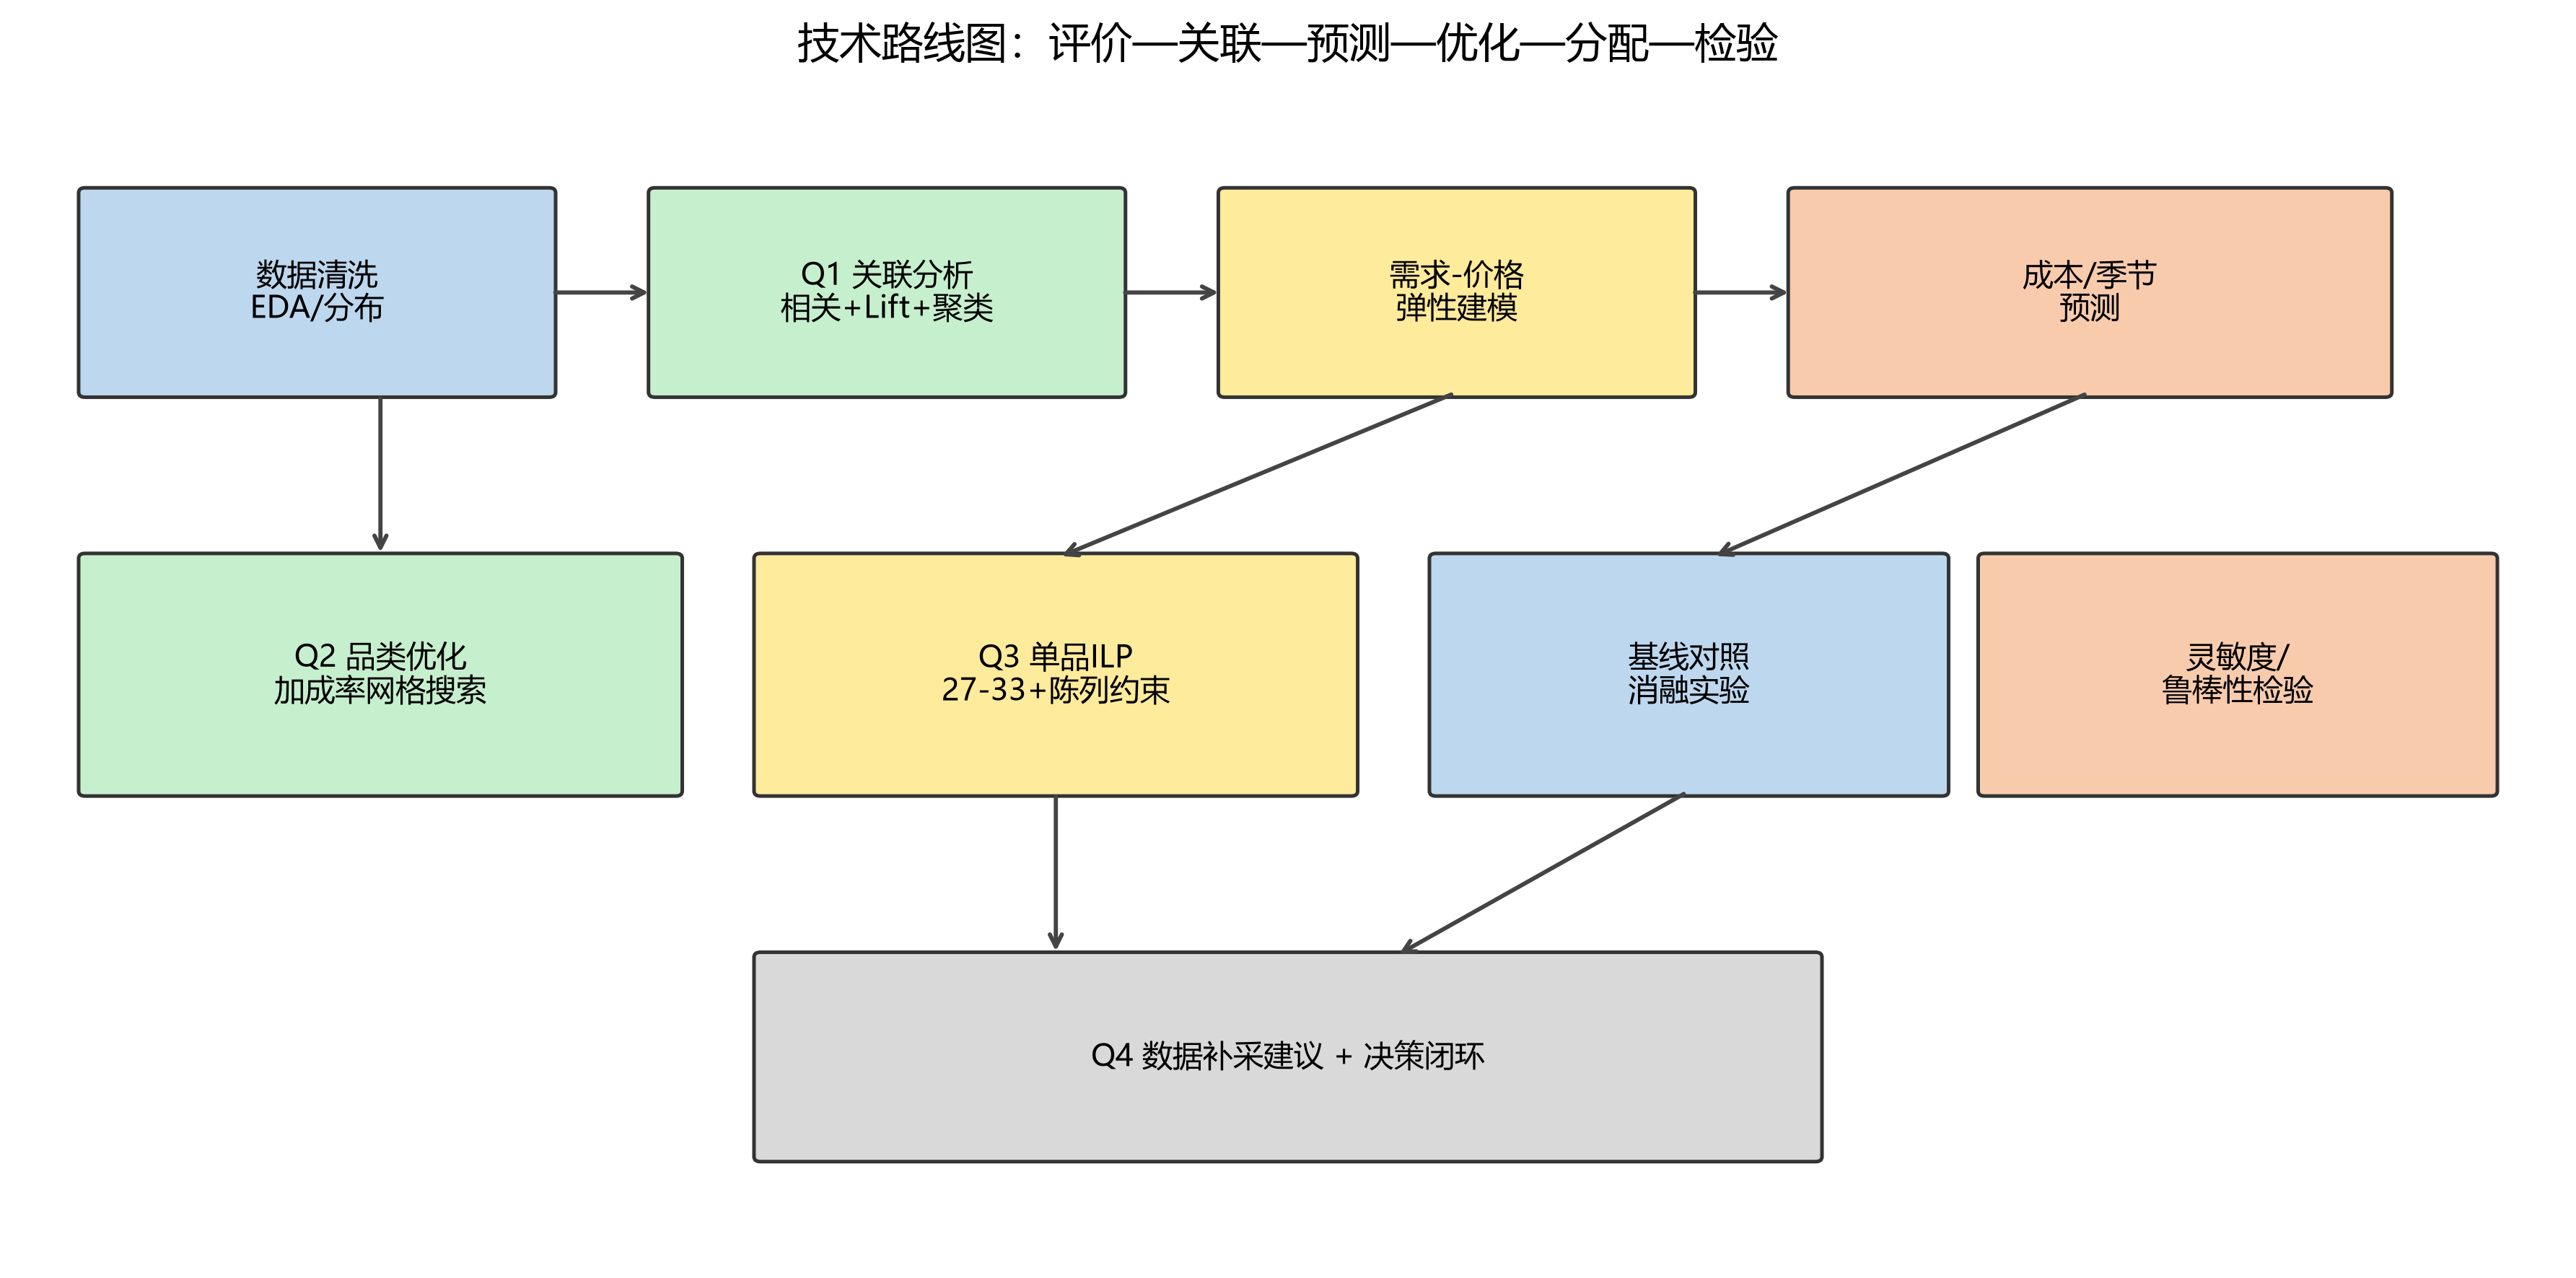
\includegraphics[width=0.98\textwidth]{figures/tech_roadmap.png}
\caption{总体技术路线图}
\label{fig:roadmap}
\end{figure}

\section{模型假设与符号说明}
\subsection{基本假设}
\begin{enumerate}[leftmargin=2em]
\item 当日未售出部分按损耗率体现，不考虑隔日再售库存结转；
\item 批发价在决策日可按近期信息预测，售价采用成本加成；
\item 需求主要由价格、成本、星期与季节因素驱动，短期内外生冲击用鲁棒性扰动刻画；
\item 小票可按``日期+分钟''近似重构，用于共现关联（存在并发误差，但方向稳健）；
\item 商超以收益最大化为主目标，品类需求满足作为Q3软约束。
\end{enumerate}

\subsection{符号说明}
\begin{table}[H]
\centering
\caption{主要符号说明}
\begin{tabular}{cl}
\toprule
符号 & 含义 \\
\midrule
$i$ & 品类或单品索引 \\
$t$ & 日期 \\
$q_{it}$ & 销量（kg） \\
$p_{it}$ & 销售单价（元/kg） \\
$c_{it}$ & 批发价（元/kg） \\
$r_{it}$ & 成本加成率，$p=c(1+r)$ \\
$\ell_i$ & 损耗率 \\
$R_{it}$ & 补货量（kg） \\
$\varepsilon_i$ & 需求价格弹性 \\
$\pi$ & 收益（元） \\
$L$ & 关联规则提升度（Lift） \\
$x_j$ & 单品$j$是否入选（0-1） \\
\bottomrule
\end{tabular}
\end{table}

\section{数据预处理与探索性分析}
对销售流水剔除非正销量/单价及极端价格后，得到干净面板。六大品类单品数与累计销量见图~\ref{fig:eda1}--\ref{fig:eda2}，月度序列与星期效应见图~\ref{fig:eda3}--\ref{fig:eda4}。描述统计见表~\ref{tab:desc}。

\begin{figure}[H]
\centering
\begin{minipage}{0.48\textwidth}
\centering
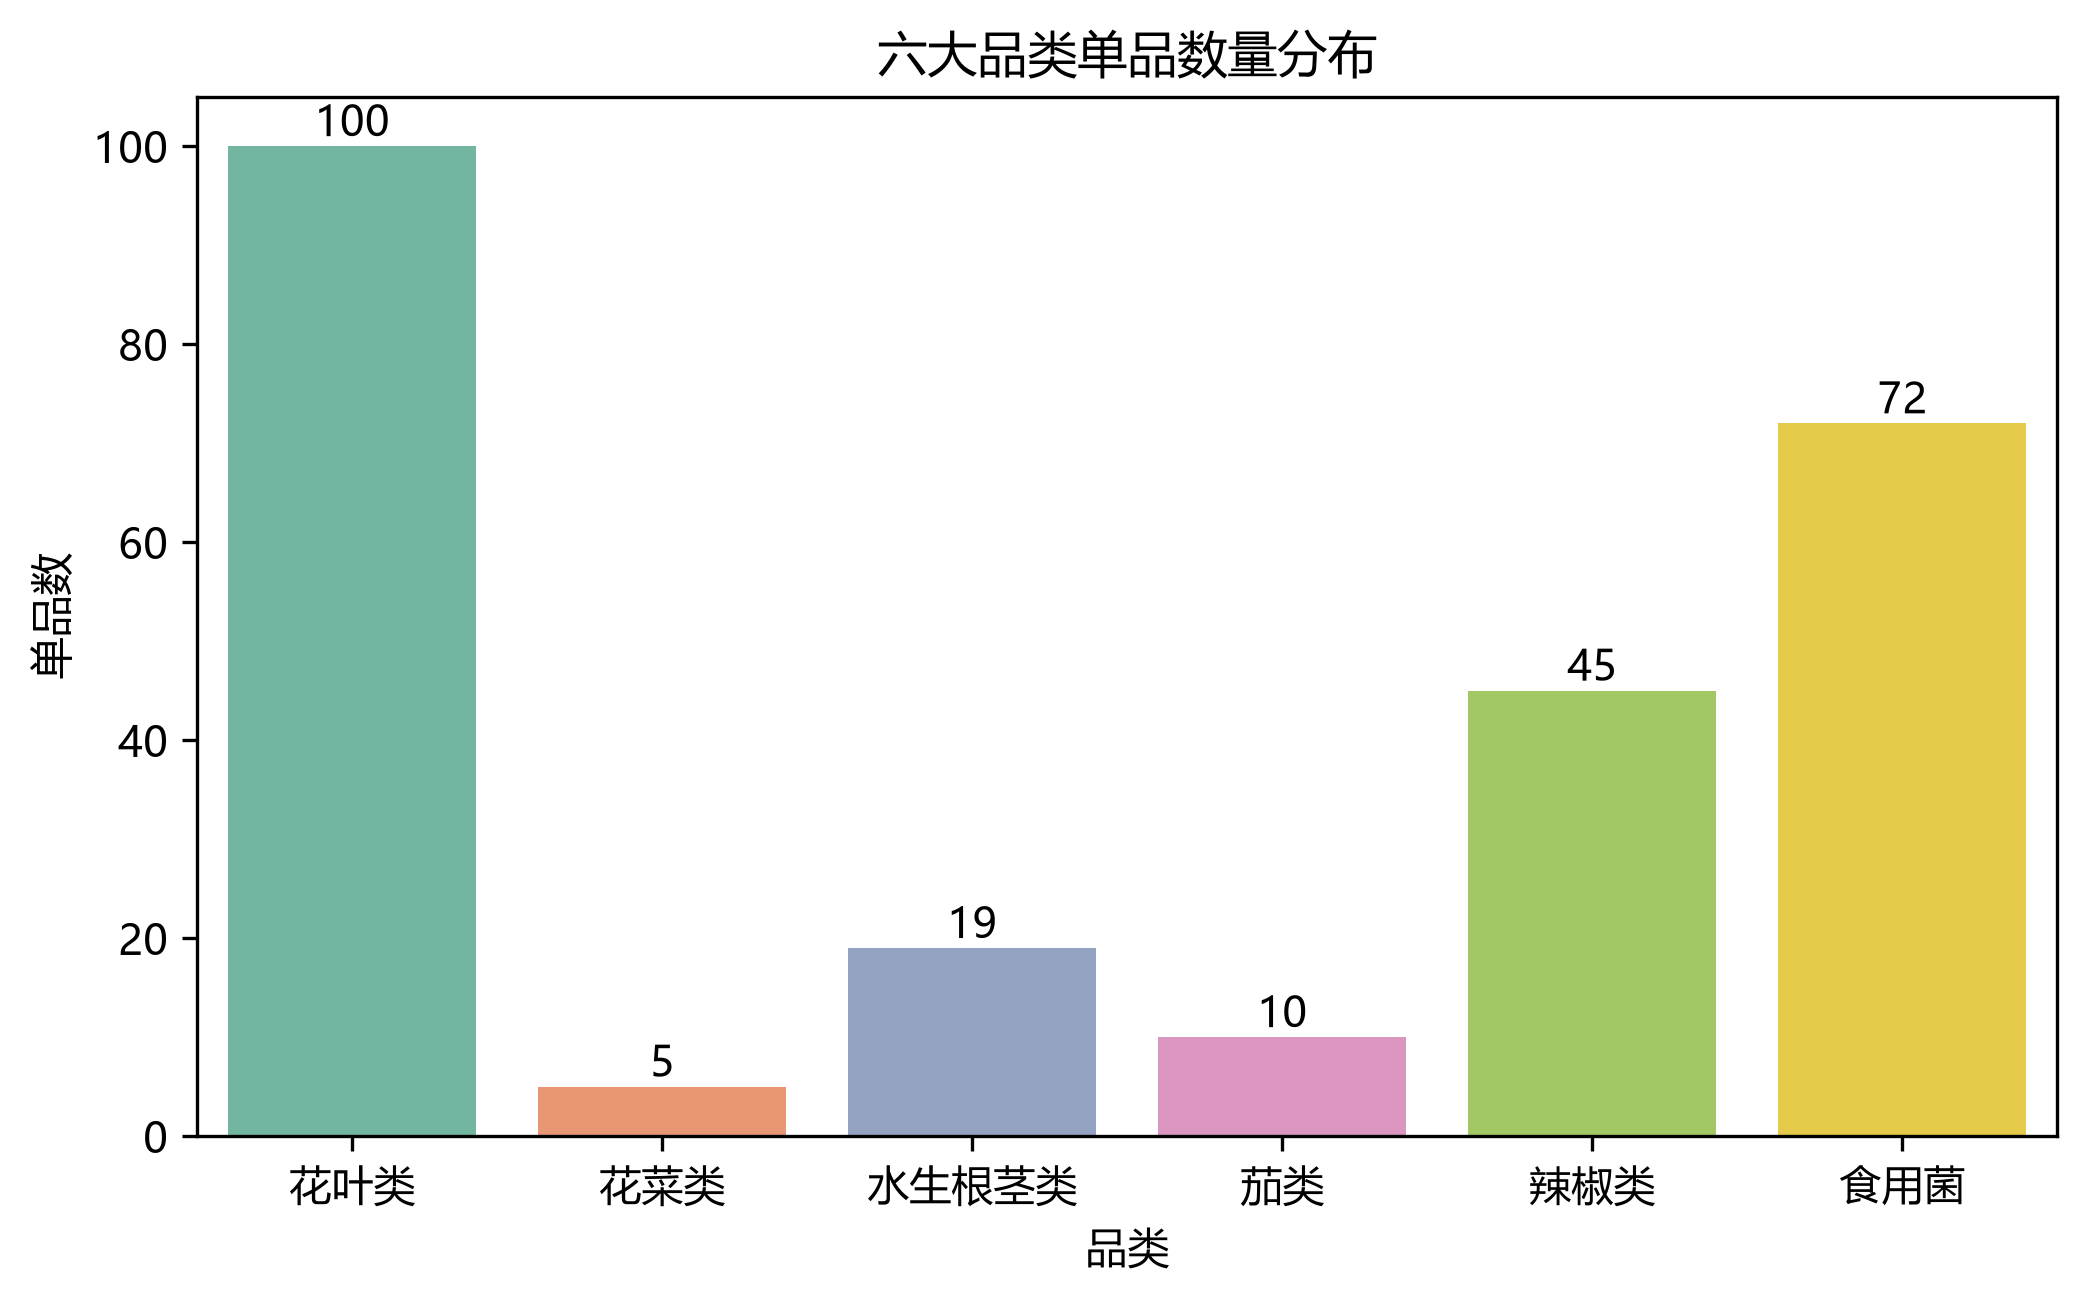
\includegraphics[width=\linewidth]{figures/eda_category_sku_count.png}
\caption{品类单品数量}
\label{fig:eda1}
\end{minipage}
\hfill
\begin{minipage}{0.48\textwidth}
\centering
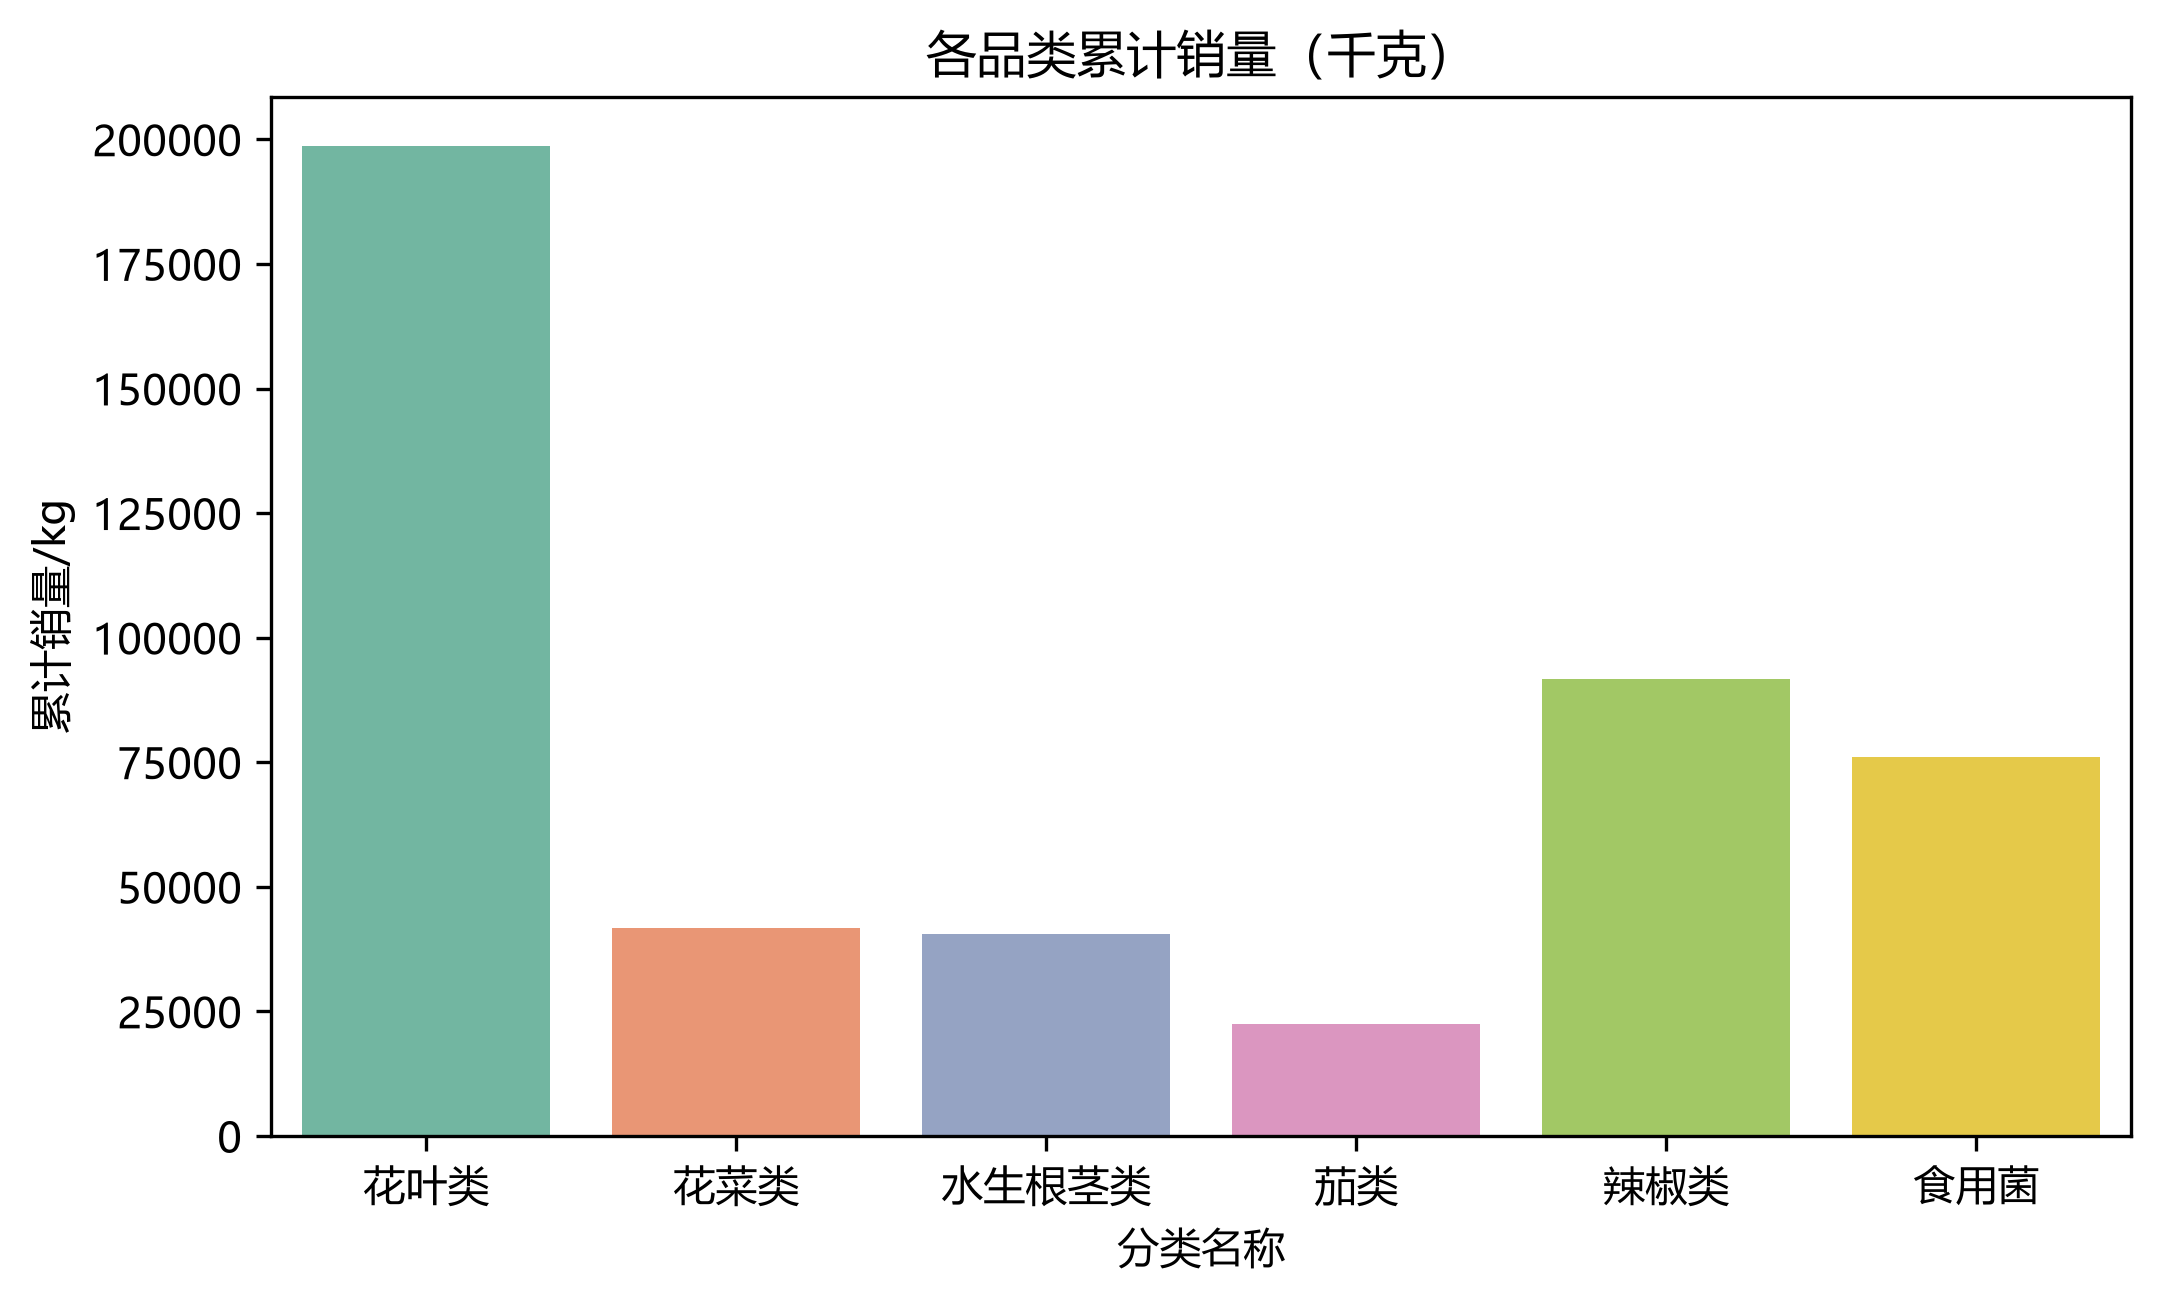
\includegraphics[width=\linewidth]{figures/eda_category_total_sales.png}
\caption{品类累计销量}
\label{fig:eda2}
\end{minipage}
\end{figure}

\begin{figure}[H]
\centering
\begin{minipage}{0.48\textwidth}
\centering
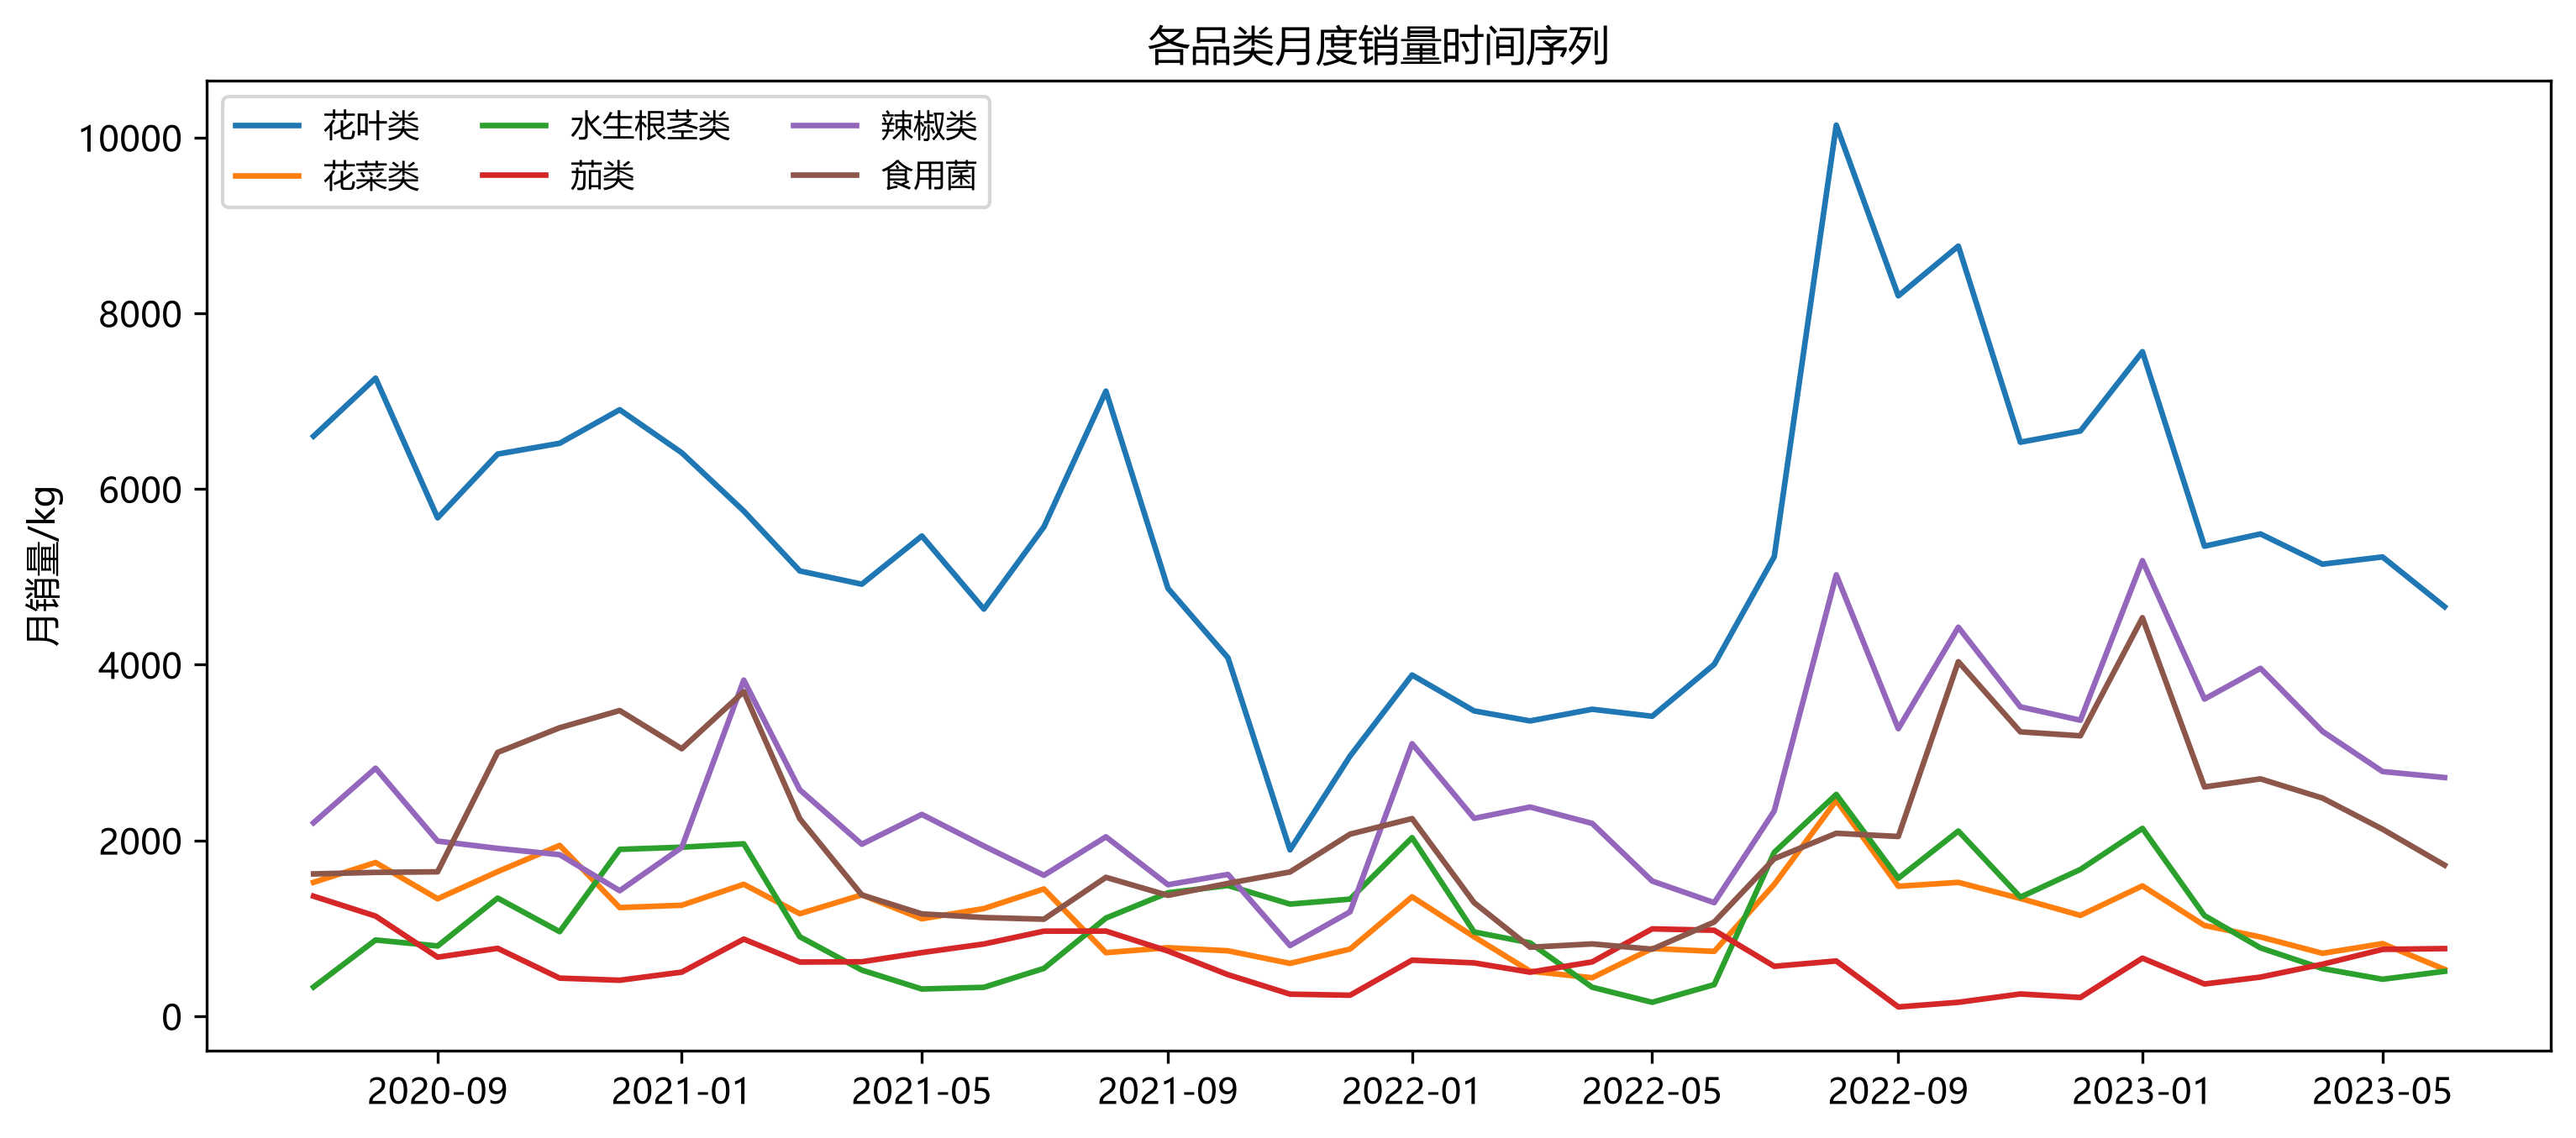
\includegraphics[width=\linewidth]{figures/eda_monthly_sales_ts.png}
\caption{月度销量序列}
\label{fig:eda3}
\end{minipage}
\hfill
\begin{minipage}{0.48\textwidth}
\centering
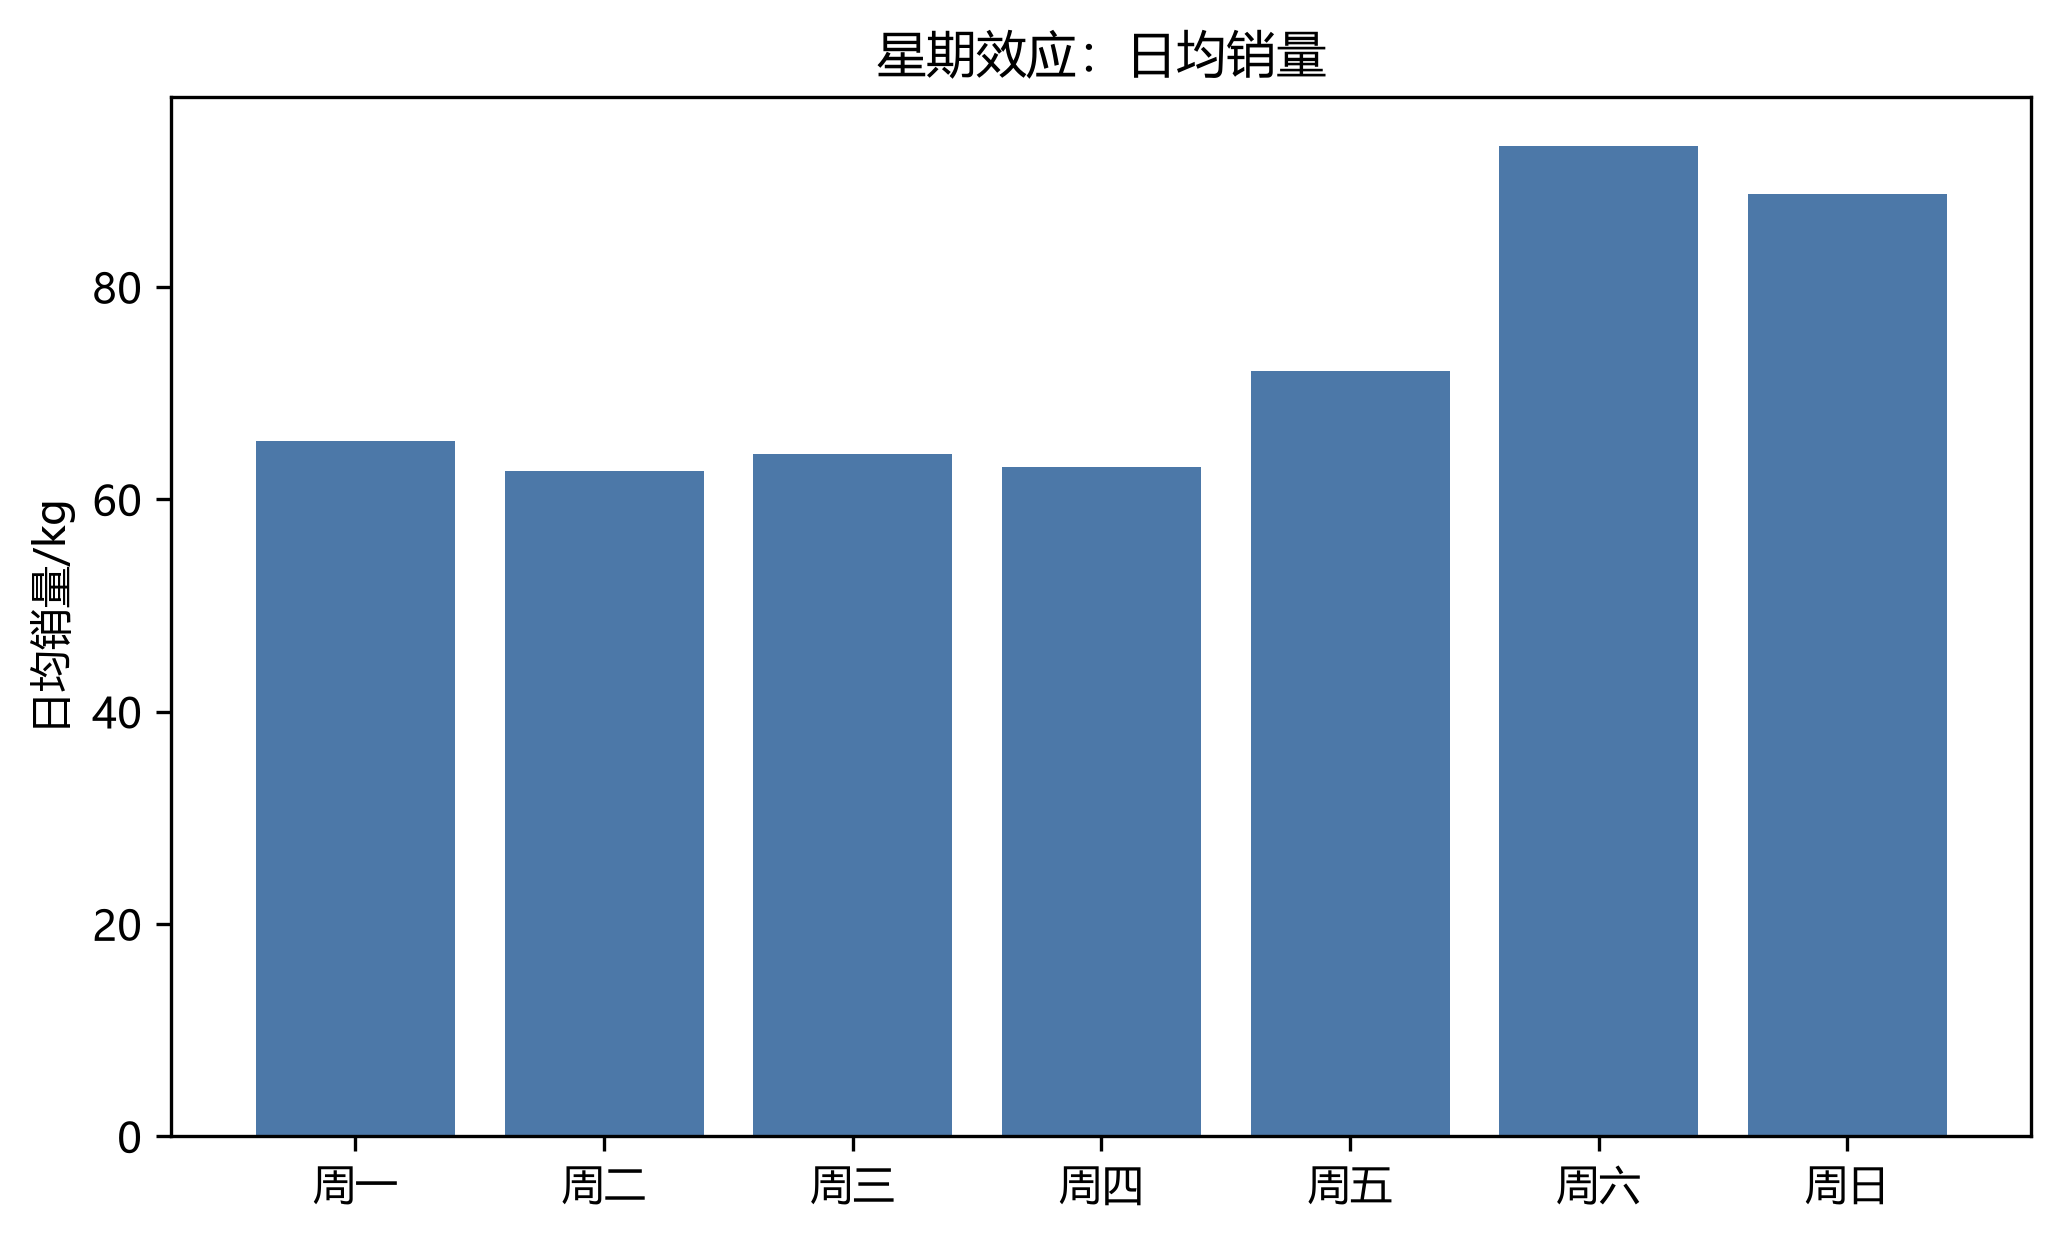
\includegraphics[width=\linewidth]{figures/eda_weekday_pattern.png}
\caption{星期效应}
\label{fig:eda4}
\end{minipage}
\end{figure}

\begin{table}[H]
\centering
\caption{品类日度描述统计}
\label{tab:desc}
\scriptsize
\begin{tabular}{lccccc}
\toprule
分类名称 & 日均销量 & 日均销售额 & 日均毛利 & 平均加成率 & 销量标准差 \\
\hline
花叶类 & 183.10 & 995.24 & 396.82 & 0.67 & 86.30 \\
花菜类 & 38.55 & 346.85 & 120.83 & 0.54 & 22.69 \\
水生根茎类 & 37.43 & 322.86 & 99.47 & 0.47 & 31.37 \\
茄类 & 21.37 & 182.12 & 66.11 & 0.59 & 13.16 \\
辣椒类 & 84.47 & 695.45 & 257.79 & 0.64 & 53.46 \\
食用菌 & 70.17 & 571.53 & 208.30 & 0.58 & 48.52 \\
\bottomrule
\end{tabular}
\end{table}

损耗率与价格分布见图~\ref{fig:loss}--\ref{fig:pricebox}，为后续``补货量=需求/(1-损耗)''口径提供依据。

\begin{figure}[H]
\centering
\begin{minipage}{0.48\textwidth}
\centering
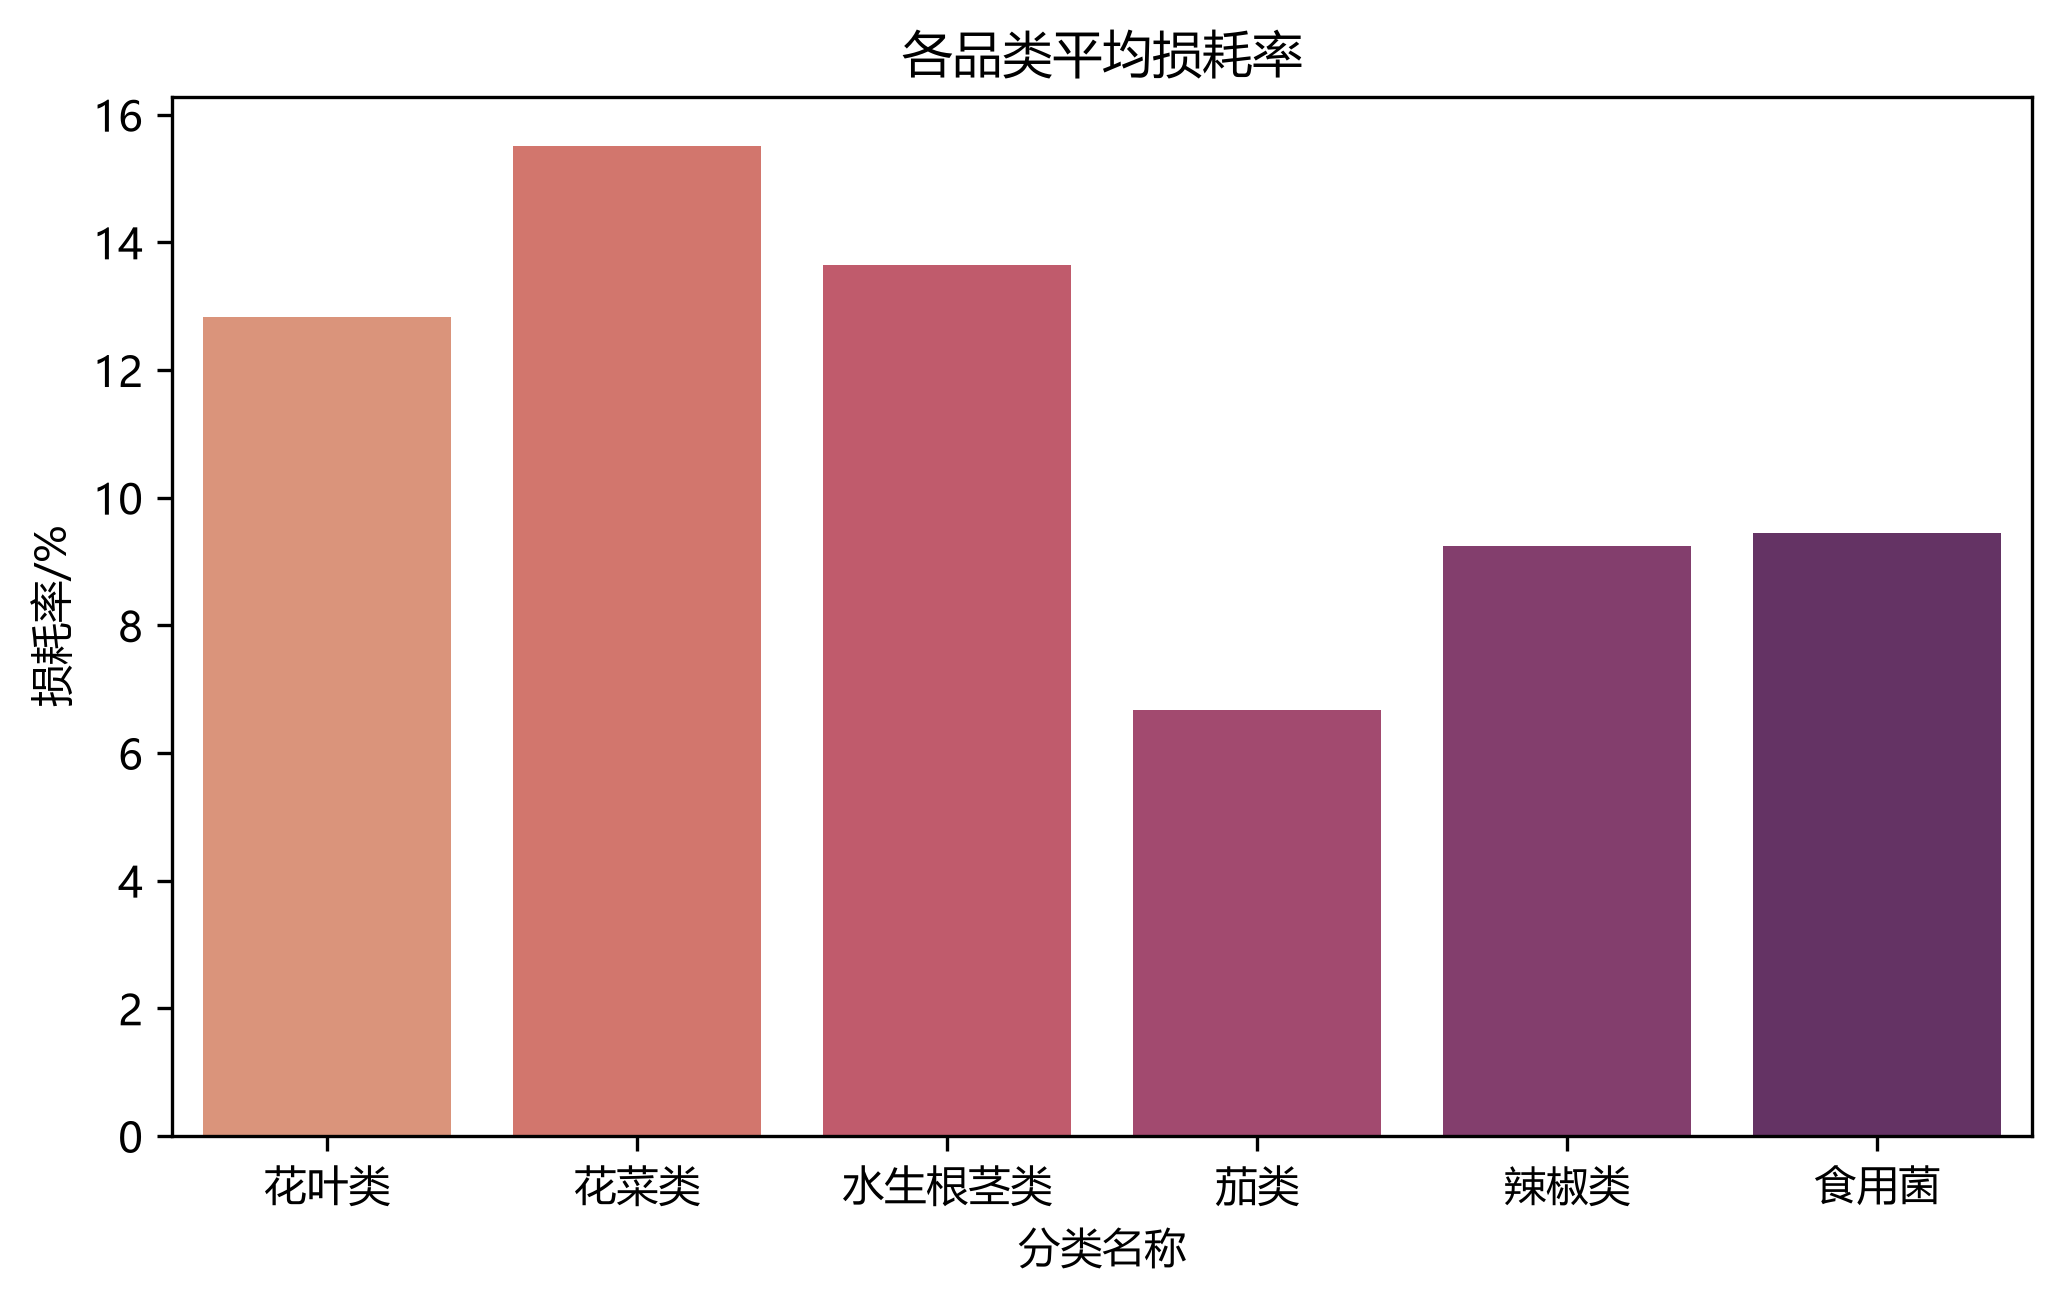
\includegraphics[width=\linewidth]{figures/eda_loss_rate.png}
\caption{品类平均损耗率}
\label{fig:loss}
\end{minipage}
\hfill
\begin{minipage}{0.48\textwidth}
\centering
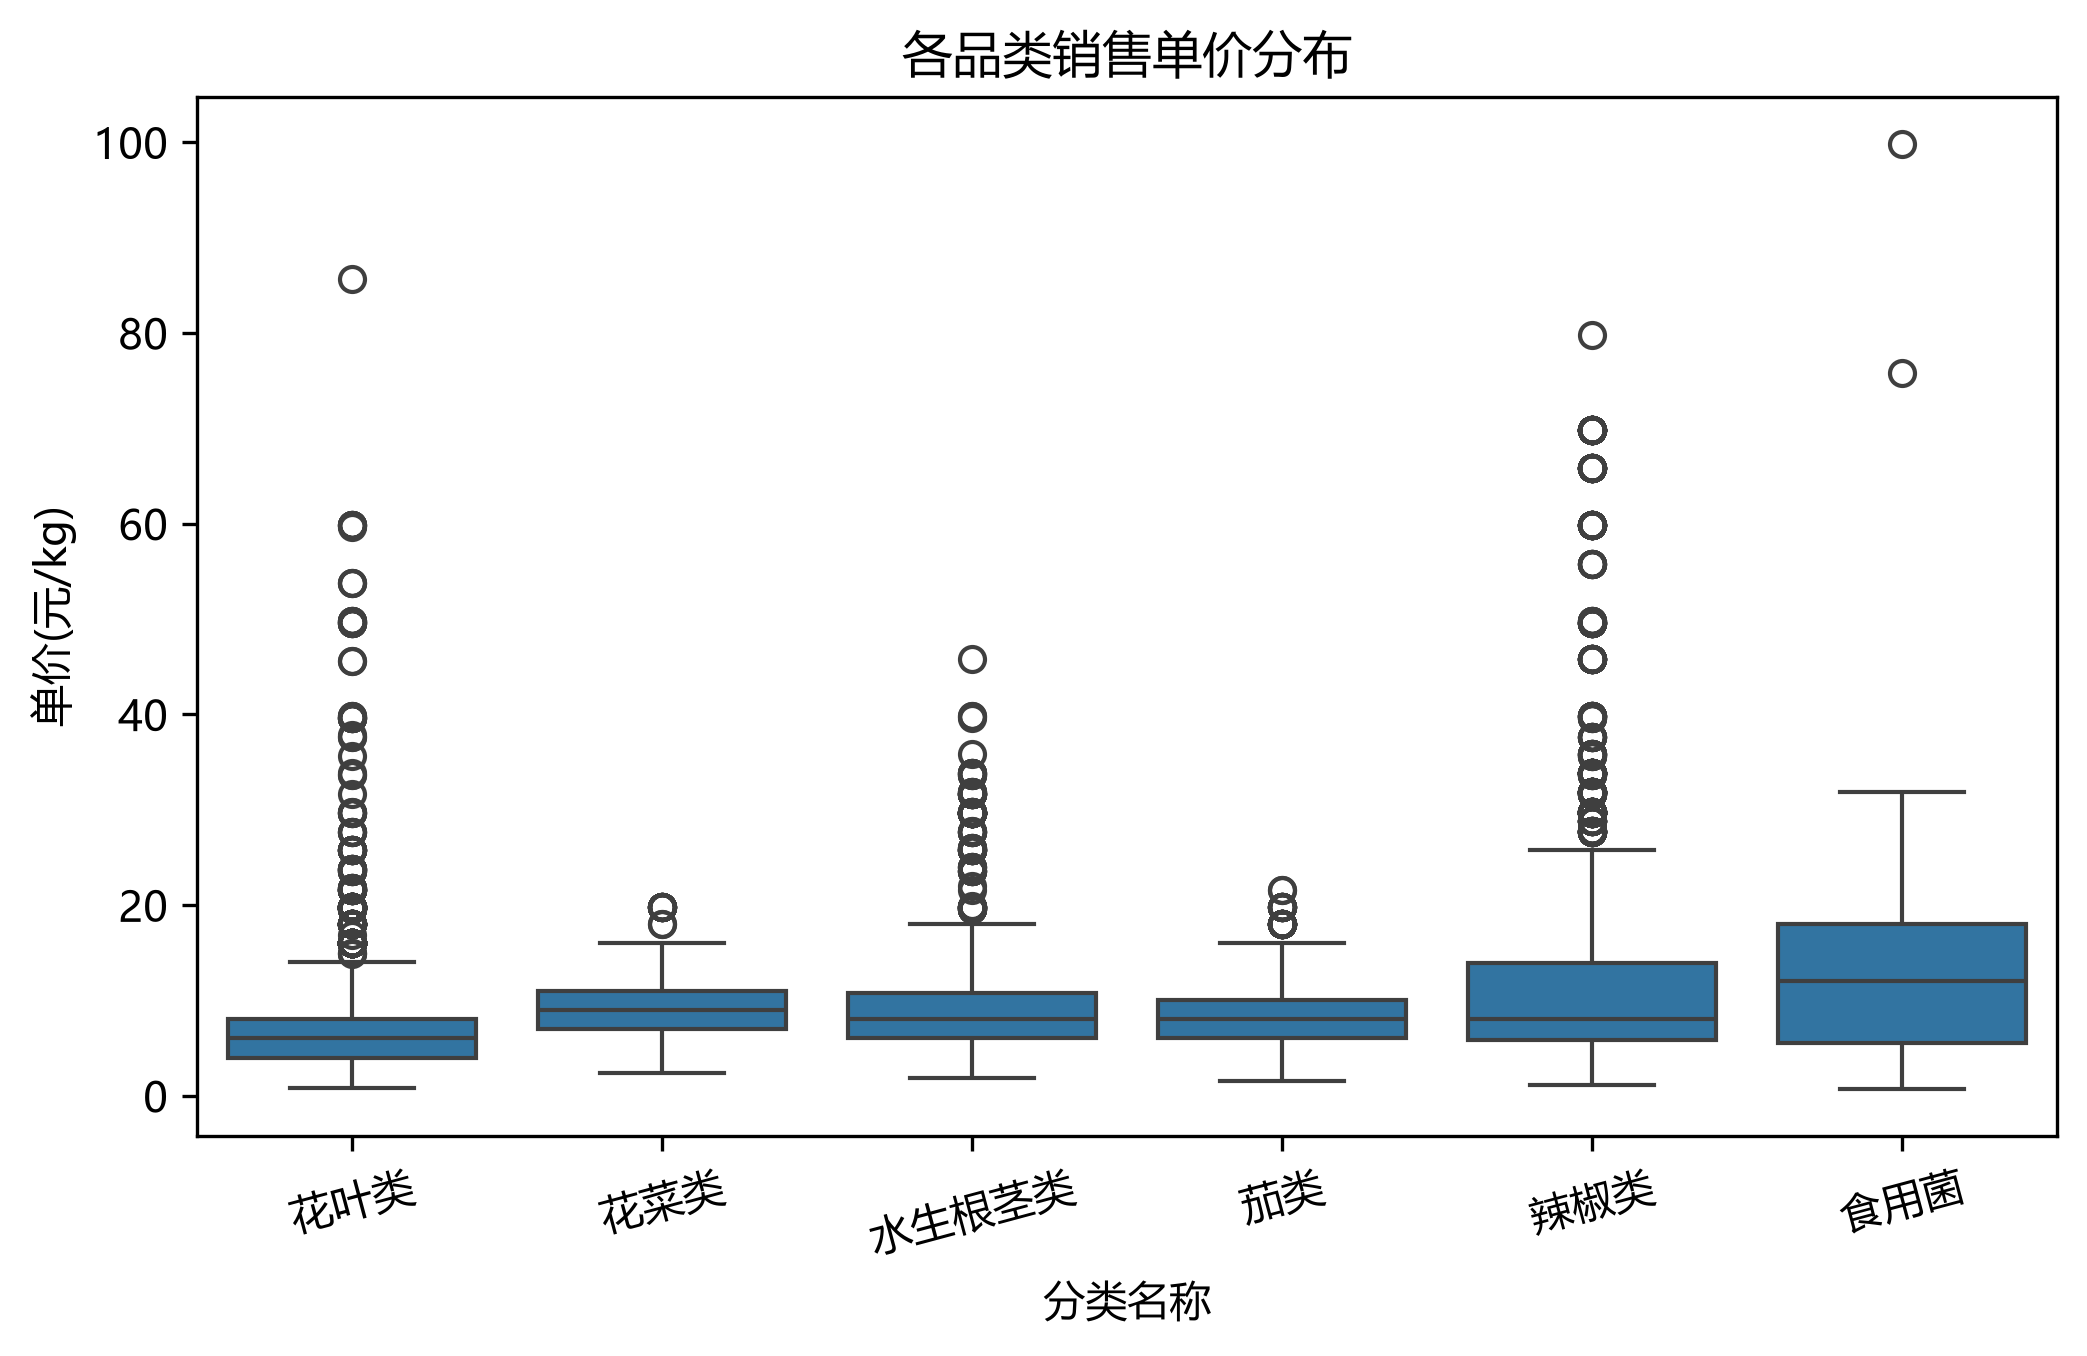
\includegraphics[width=\linewidth]{figures/eda_price_boxplot.png}
\caption{品类单价分布}
\label{fig:pricebox}
\end{minipage}
\end{figure}

\section{问题1：分布规律与关联关系}
\subsection{问题定位}
Q1回答``卖什么、一起卖什么''，为后续选品多样性与交叉销售提供结构信息。

\subsection{模型}
\subsubsection{分布拟合}
对品类日销量$q$比较正态分布、对数正态与Gamma，以KS统计量选优。偏度与峰度用于描述右尾与突发需求。

\subsubsection{相关分析}
构造品类--日期销量矩阵$Q$，计算
\begin{equation}
\rho_{ij}^{\mathrm{P}}=\mathrm{Corr}(Q_{\cdot i},Q_{\cdot j}),\quad
\rho_{ij}^{\mathrm{S}}=\mathrm{Spearman}(Q_{\cdot i},Q_{\cdot j}).
\end{equation}
二者上三角一致性用于稳健性核对。

\subsubsection{关联规则}
以近似小票篮筐计算支持度、置信度与提升度\cite{assoc}：
\begin{align}
\mathrm{supp}(A\cup B)&=\frac{|T_{A\cap B}|}{|T|},\\
\mathrm{conf}(A\to B)&=\frac{\mathrm{supp}(A\cup B)}{\mathrm{supp}(A)},\\
\mathrm{lift}(A\to B)&=\frac{\mathrm{conf}(A\to B)}{\mathrm{supp}(B)}.
\end{align}
$\mathrm{lift}>1$表示正向共购关联。

\subsubsection{单品聚类}
对活跃单品提取日均销量、波动、均价、活跃天数与加成率，标准化后做K-Means，并以轮廓系数选择$K$\cite{cluster}。短期需求外推亦参考预测实践\cite{forecast}。

\subsection{结果与分析}
分布拟合结果见表~\ref{tab:dist}与图~\ref{fig:dist}。相关热力图见图~\ref{fig:corr}，Lift热力图与Top规则见图~\ref{fig:lift}--\ref{fig:toplift}，规则表见表~\ref{tab:rules}。单品聚类见图~\ref{fig:cluster}（$K$=3，轮廓系数=0.441）。

从经营解释看，日销量相关刻画的是\textbf{宏观同步}：客流、天气、节假日等共同冲击会抬高多数品类，因而花叶类与食用菌、辣椒类等往往同向波动。提升度刻画的是\textbf{微观共购}：同一小票内的搭配结构。本文结果显示相关较强的品类对，其Lift未必显著大于1，说明``一起卖得好''不等于``经常被同一顾客同时购买''。对补货而言，相关更适合指导\textbf{品类总量备货}，Lift更适合指导\textbf{陈列邻近与组合促销}；二者不可互相替代。

聚类把单品分成高销量低波动、中等销量高溢价、长尾低活跃等类型。后续Q3在27--33的名额约束下，应优先覆盖高贡献簇，并用长尾簇中的代表性单品维持品类完整性，而不是简单按销量Top截断。

\begin{table}[H]
\centering
\caption{品类销量分布拟合}
\label{tab:dist}
\scriptsize
\begin{tabular}{lccccc}
\toprule
品类 & 均值 & 标准差 & 偏度 & 最优分布 & KS统计量 \\
\hline
花叶类 & 183.10 & 86.26 & 2.89 & lognorm & 0.02 \\
花菜类 & 38.55 & 22.68 & 1.52 & lognorm & 0.02 \\
水生根茎类 & 37.43 & 31.35 & 2.50 & lognorm & 0.05 \\
茄类 & 21.37 & 13.16 & 1.74 & lognorm & 0.01 \\
辣椒类 & 84.47 & 53.44 & 3.14 & lognorm & 0.03 \\
食用菌 & 70.17 & 48.50 & 2.99 & lognorm & 0.03 \\
\bottomrule
\end{tabular}
\end{table}

\begin{figure}[H]
\centering
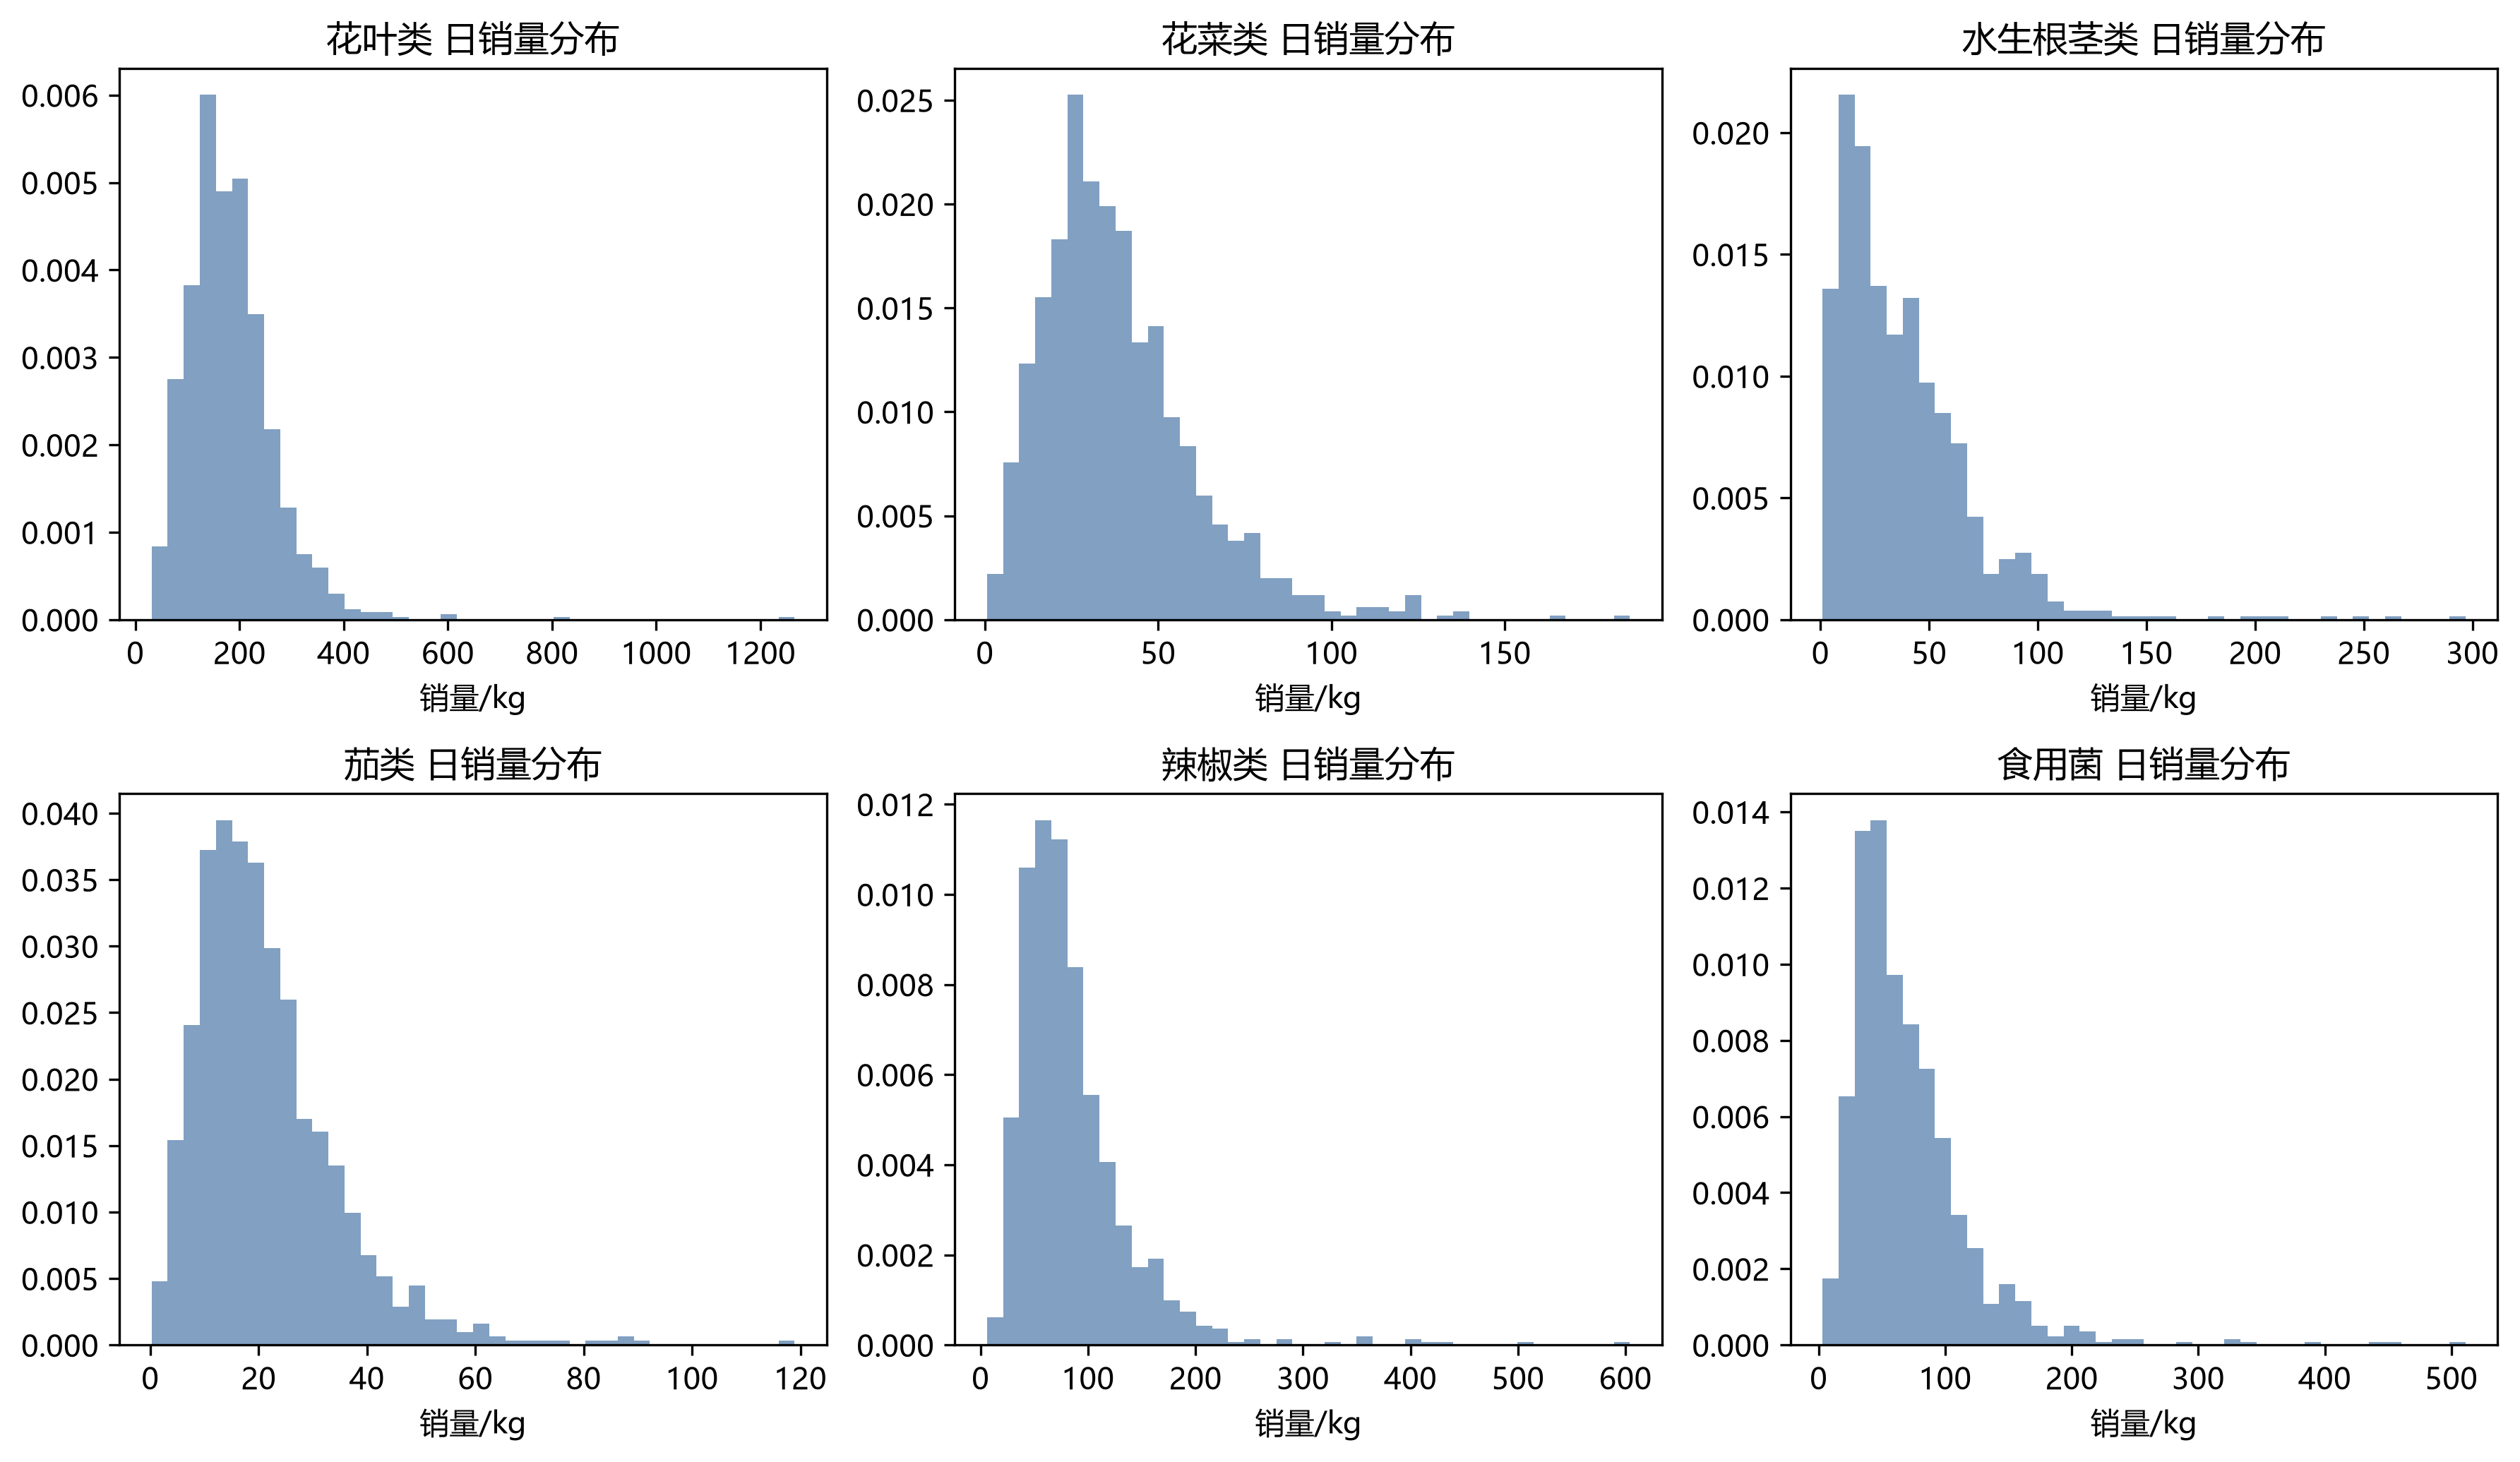
\includegraphics[width=0.95\textwidth]{figures/q1_category_dist_fit.png}
\caption{各品类日销量分布}
\label{fig:dist}
\end{figure}

\begin{figure}[H]
\centering
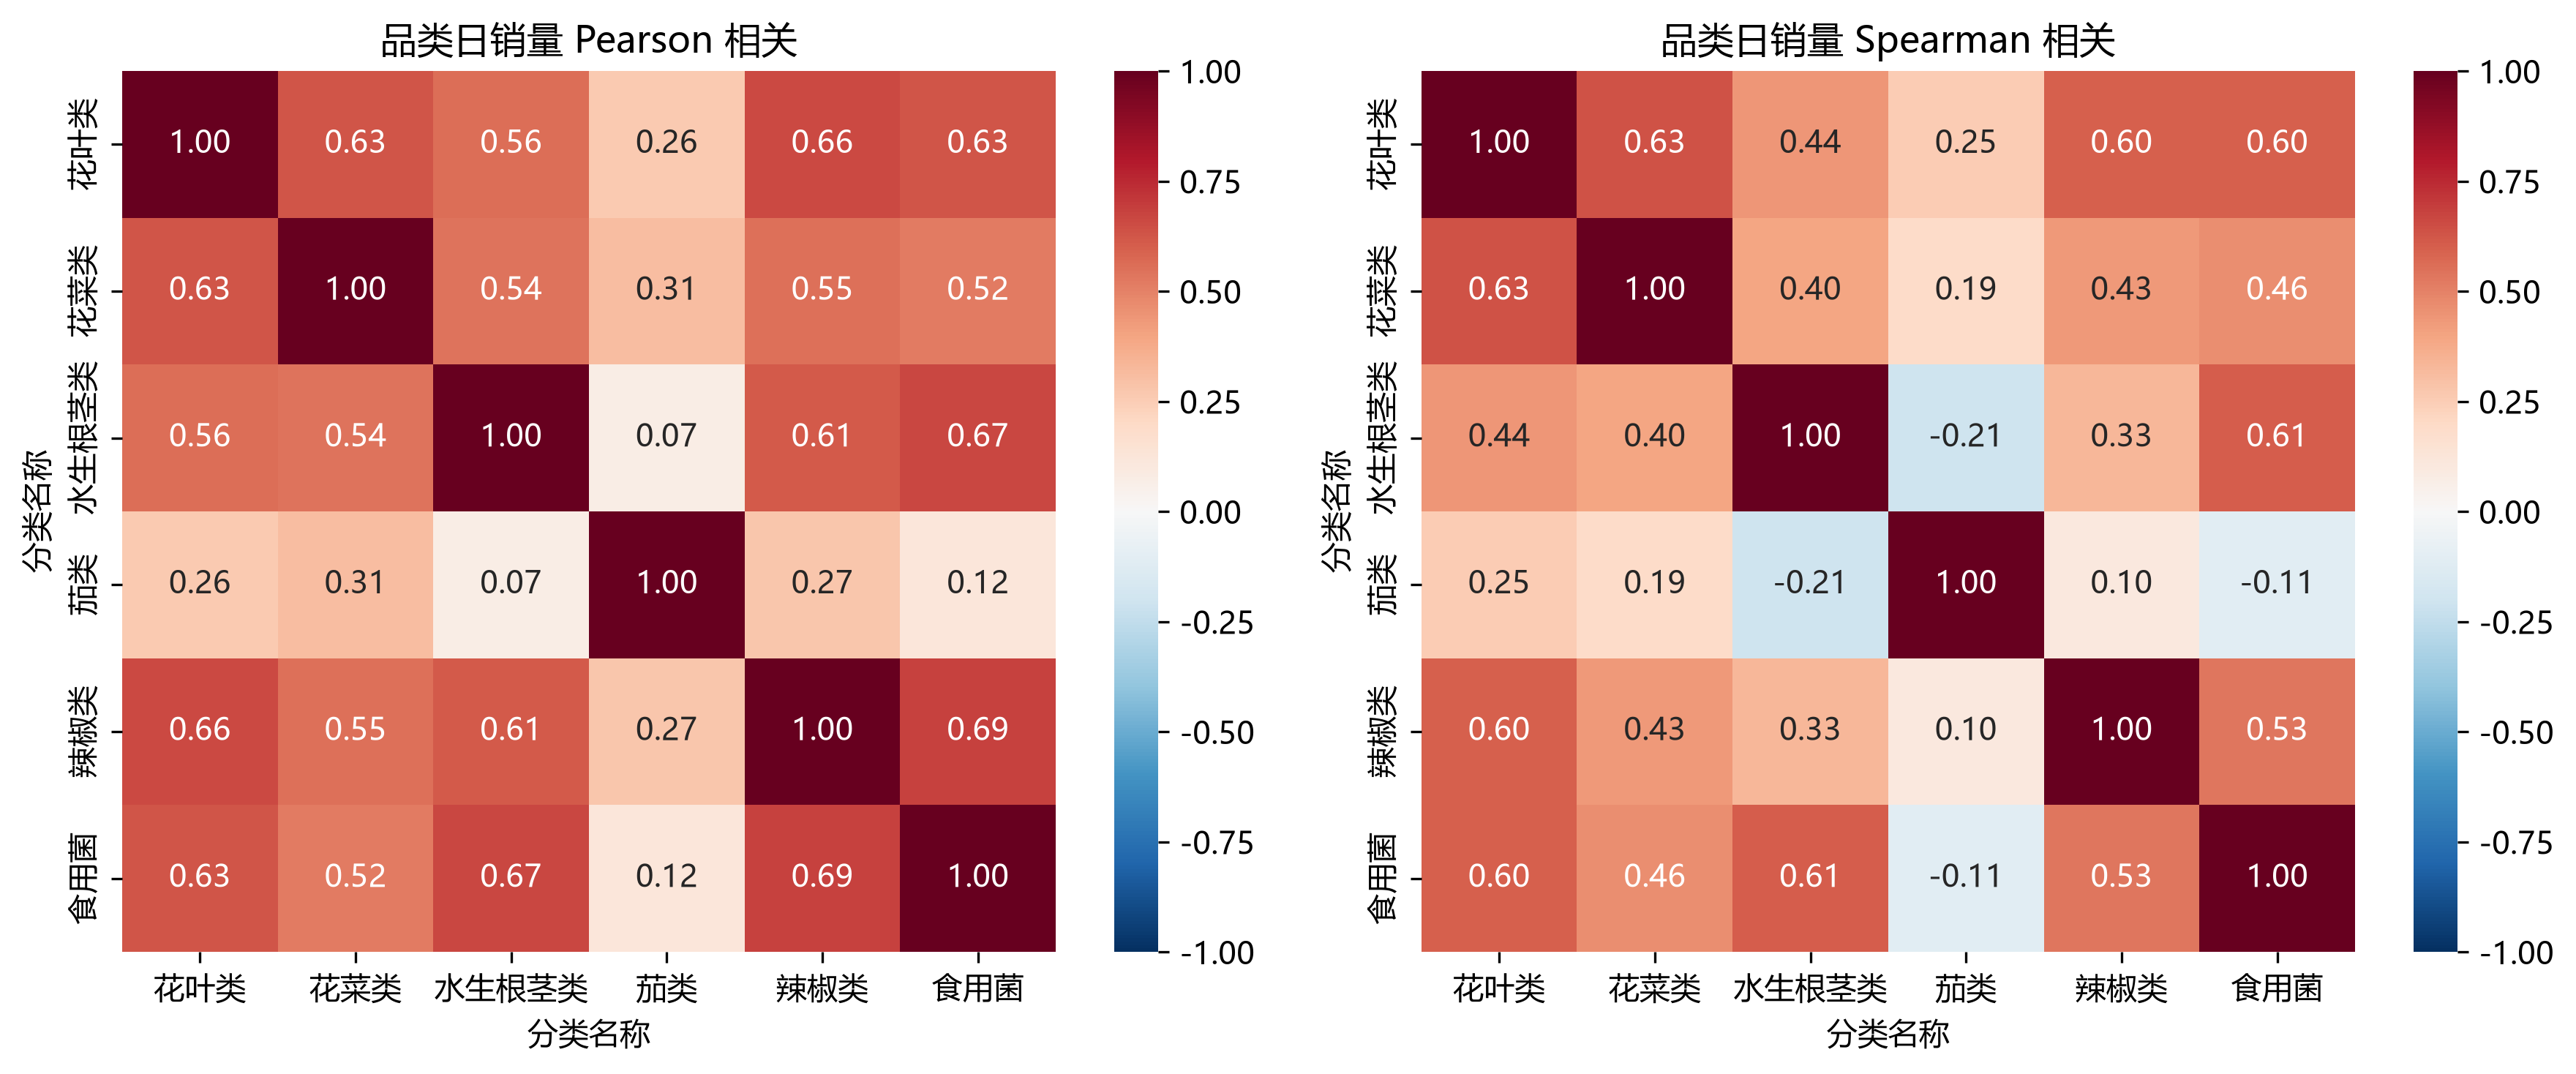
\includegraphics[width=0.95\textwidth]{figures/q1_category_corr_heatmap.png}
\caption{品类日销量相关热力图}
\label{fig:corr}
\end{figure}

\begin{figure}[H]
\centering
\begin{minipage}{0.48\textwidth}
\centering
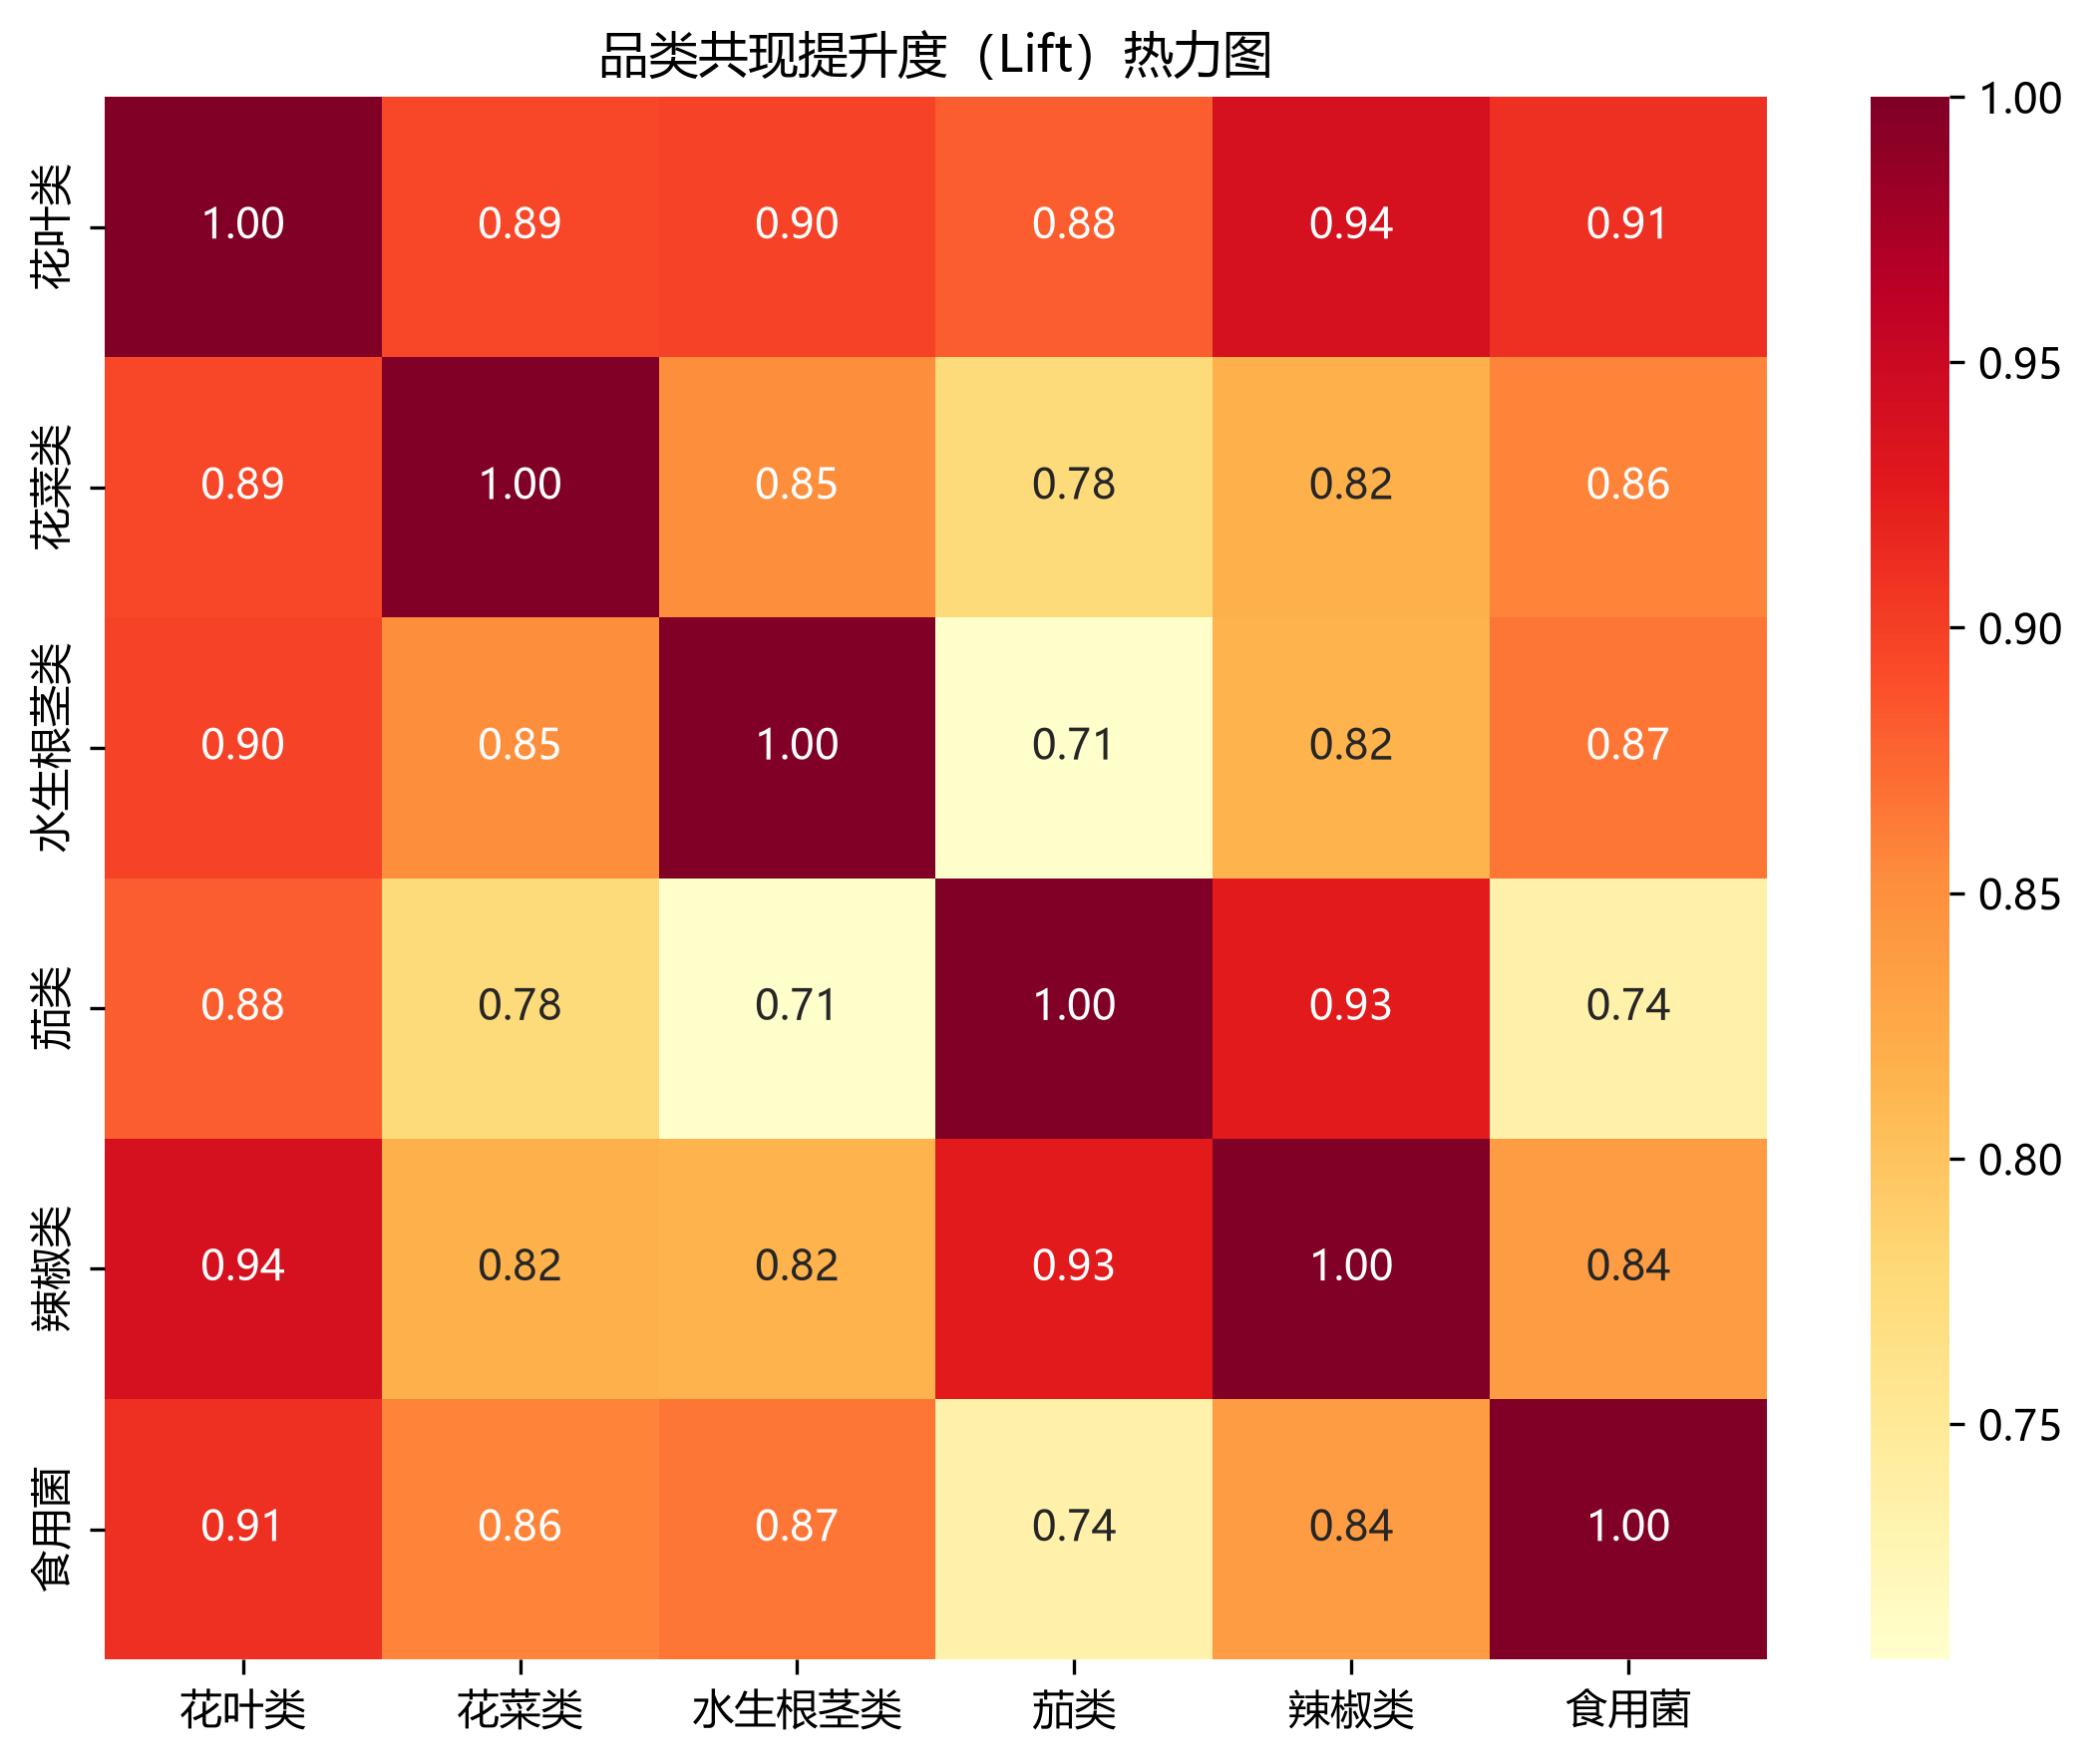
\includegraphics[width=\linewidth]{figures/q1_association_lift.png}
\caption{品类共现Lift}
\label{fig:lift}
\end{minipage}
\hfill
\begin{minipage}{0.48\textwidth}
\centering
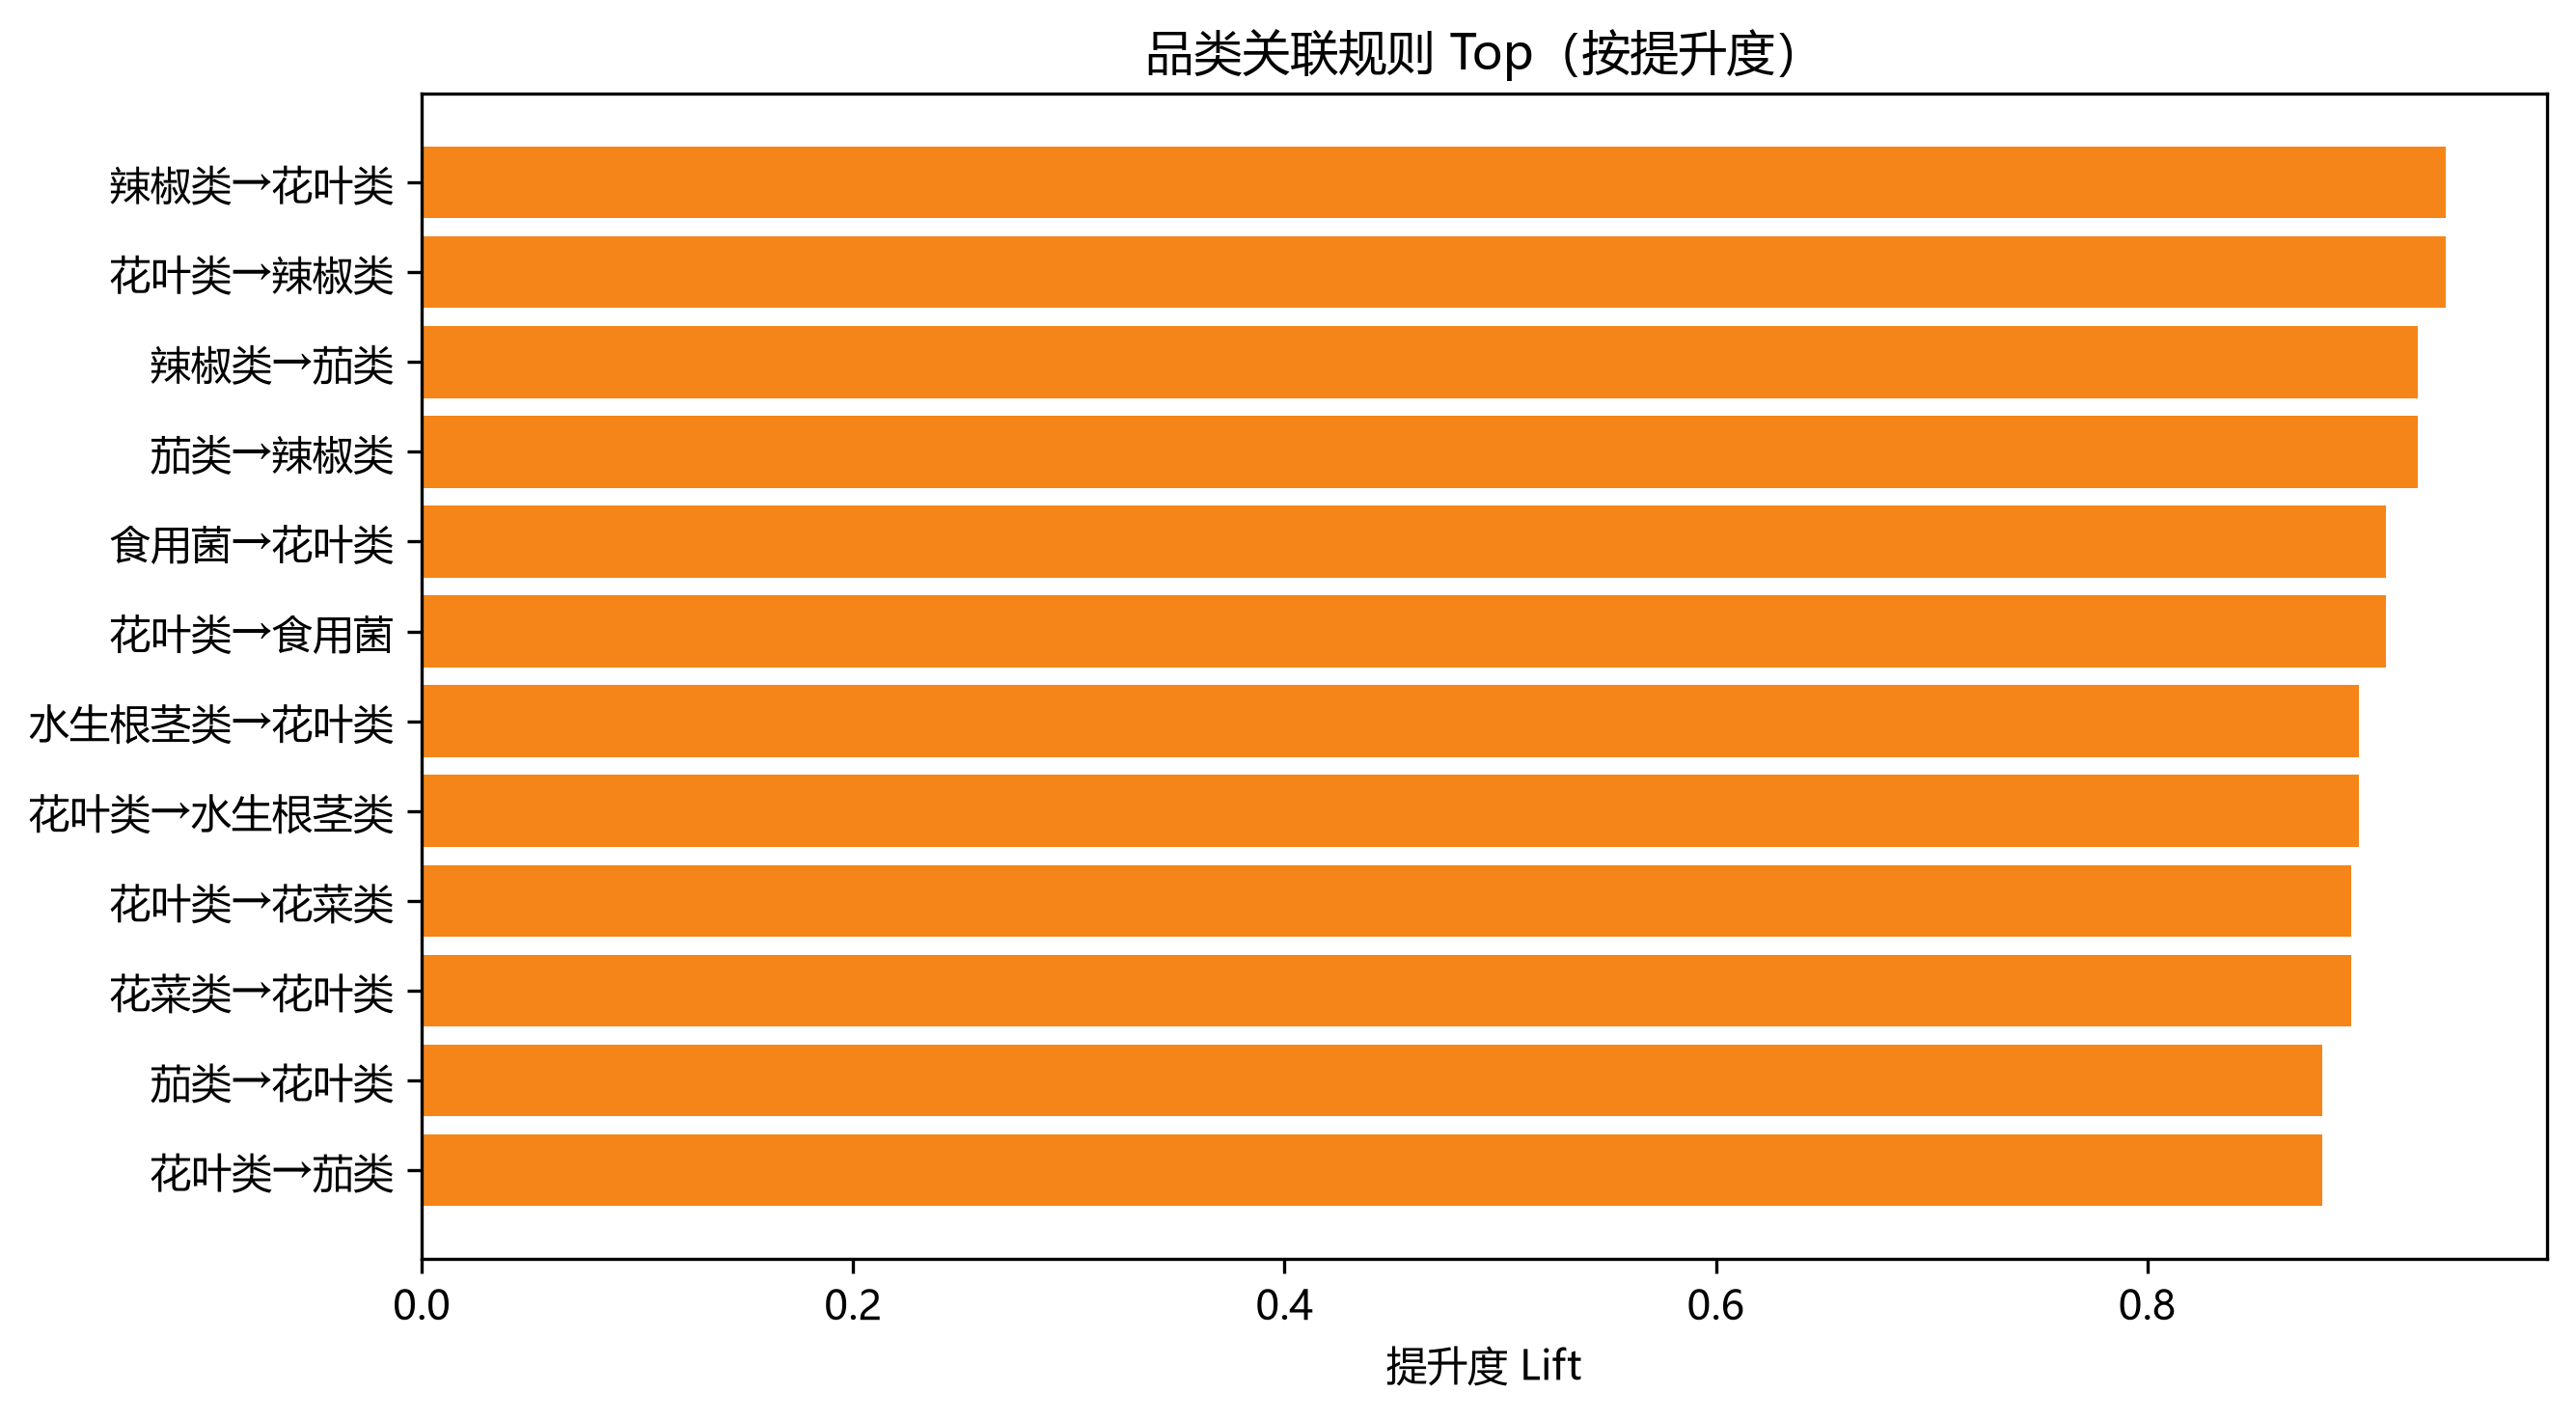
\includegraphics[width=\linewidth]{figures/q1_top_lift_rules.png}
\caption{Top提升度规则}
\label{fig:toplift}
\end{minipage}
\end{figure}

\begin{table}[H]
\centering
\caption{品类关联规则（节选）}
\label{tab:rules}
\scriptsize
\begin{tabular}{lcccc}
\toprule
前项 & 后项 & 支持度 & 置信度A至B & 提升度 \\
\hline
辣椒类 & 花叶类 & 0.42 & 0.70 & 0.94 \\
花叶类 & 辣椒类 & 0.42 & 0.56 & 0.94 \\
辣椒类 & 茄类 & 0.10 & 0.17 & 0.93 \\
茄类 & 辣椒类 & 0.10 & 0.55 & 0.93 \\
食用菌 & 花叶类 & 0.32 & 0.68 & 0.91 \\
花叶类 & 食用菌 & 0.32 & 0.42 & 0.91 \\
水生根茎类 & 花叶类 & 0.15 & 0.67 & 0.90 \\
花叶类 & 水生根茎类 & 0.15 & 0.19 & 0.90 \\
\bottomrule
\end{tabular}
\end{table}

\begin{figure}[H]
\centering
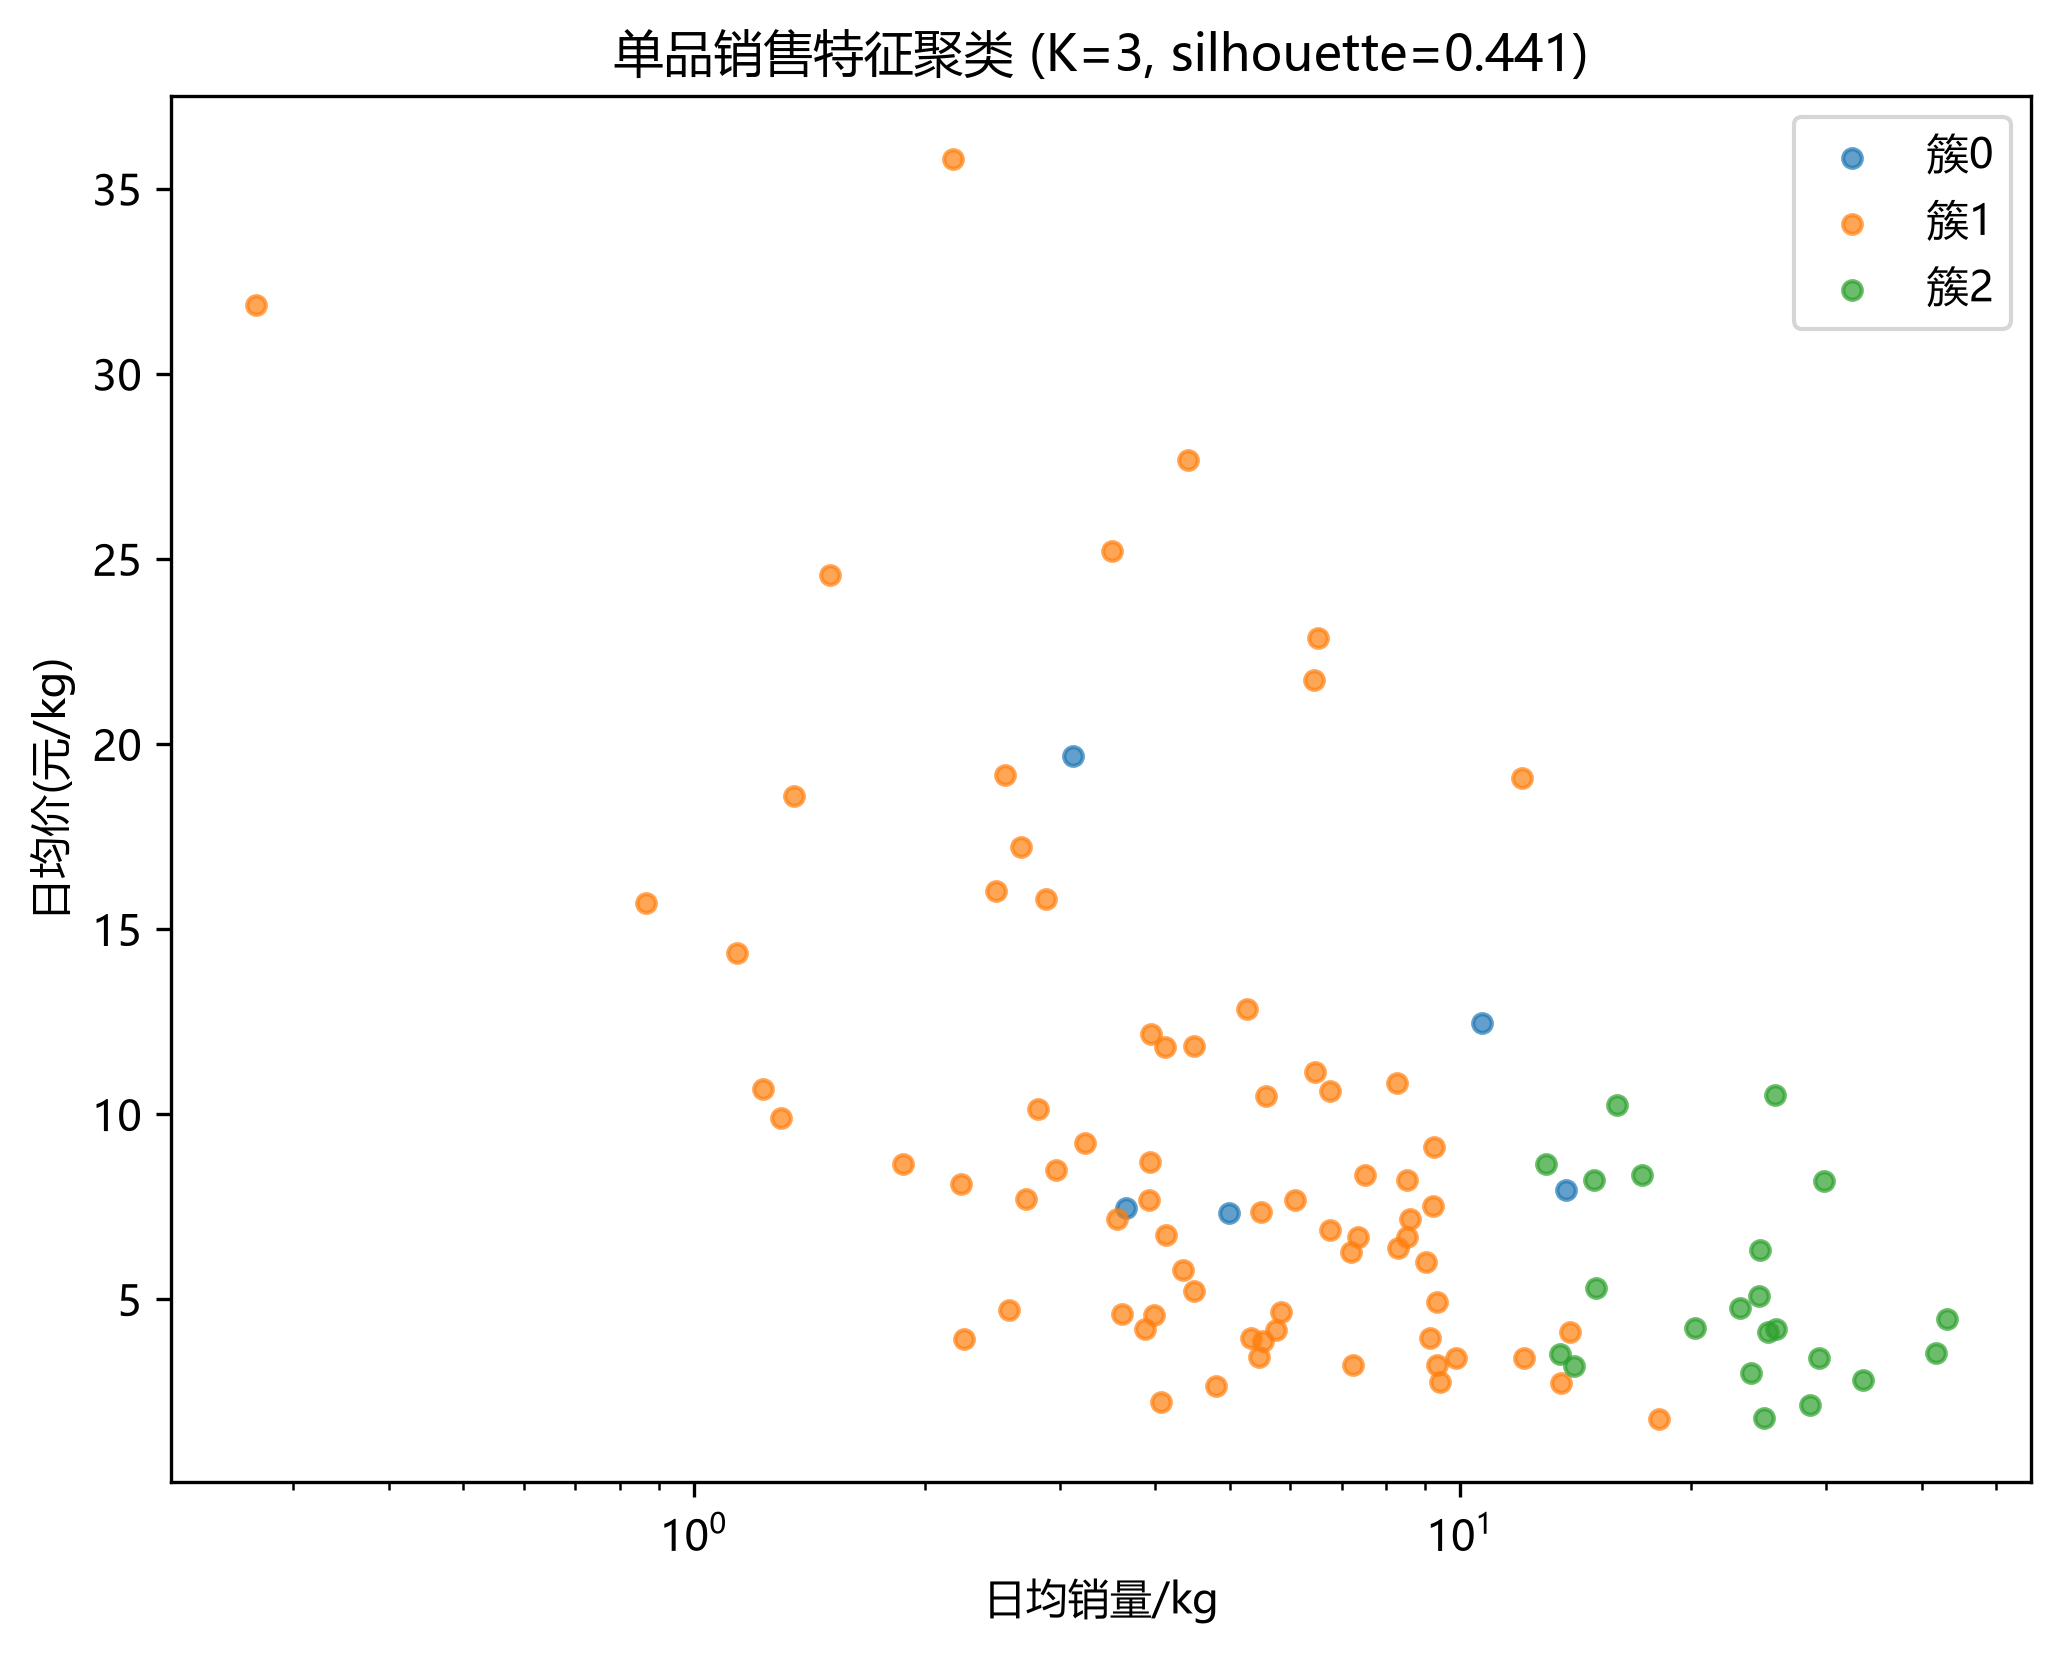
\includegraphics[width=0.85\textwidth]{figures/q1_sku_clusters.png}
\caption{单品销售特征聚类}
\label{fig:cluster}
\end{figure}

\subsection{与下一问衔接}
Q1表明品类需求同步波动显著，但共购结构并不等同于相关结构；因此Q2先在品类层优化``总量+定价''，Q3再把总量分解到具有差异化贡献的单品组合。

\section{问题2：品类补货与定价}
\subsection{问题定位}
在品类层最大化未来一周收益，输出每日补货总量与售价。

\subsection{需求--价格模型}
采用对数线性市场反应模型\cite{elast,pricing}：
\begin{equation}
\ln q_{it}=\alpha_i+\varepsilon_i\ln p_{it}+\gamma_i\ln c_{it}+\sum_{d} \beta_{id}W_{td}+\sum_{m}\delta_{im}M_{tm}+u_{it},
\end{equation}
其中$W$、$M$为星期与月份控制。估计用Ridge回归\cite{ridge}，并以时间序列交叉验证报告MAE，相对``均值预测基线''计算提升。售价决策与收益管理思想一致\cite{bilevel,pricing}，损耗下的订货匹配参考报童类供需匹配框架\cite{newsvendor,loss}。

价格--销量散点与弹性估计见图~\ref{fig:scatter}--\ref{fig:elast}，弹性表见表~\ref{tab:elast}。残差诊断见图~\ref{fig:resid}。

\begin{figure}[H]
\centering
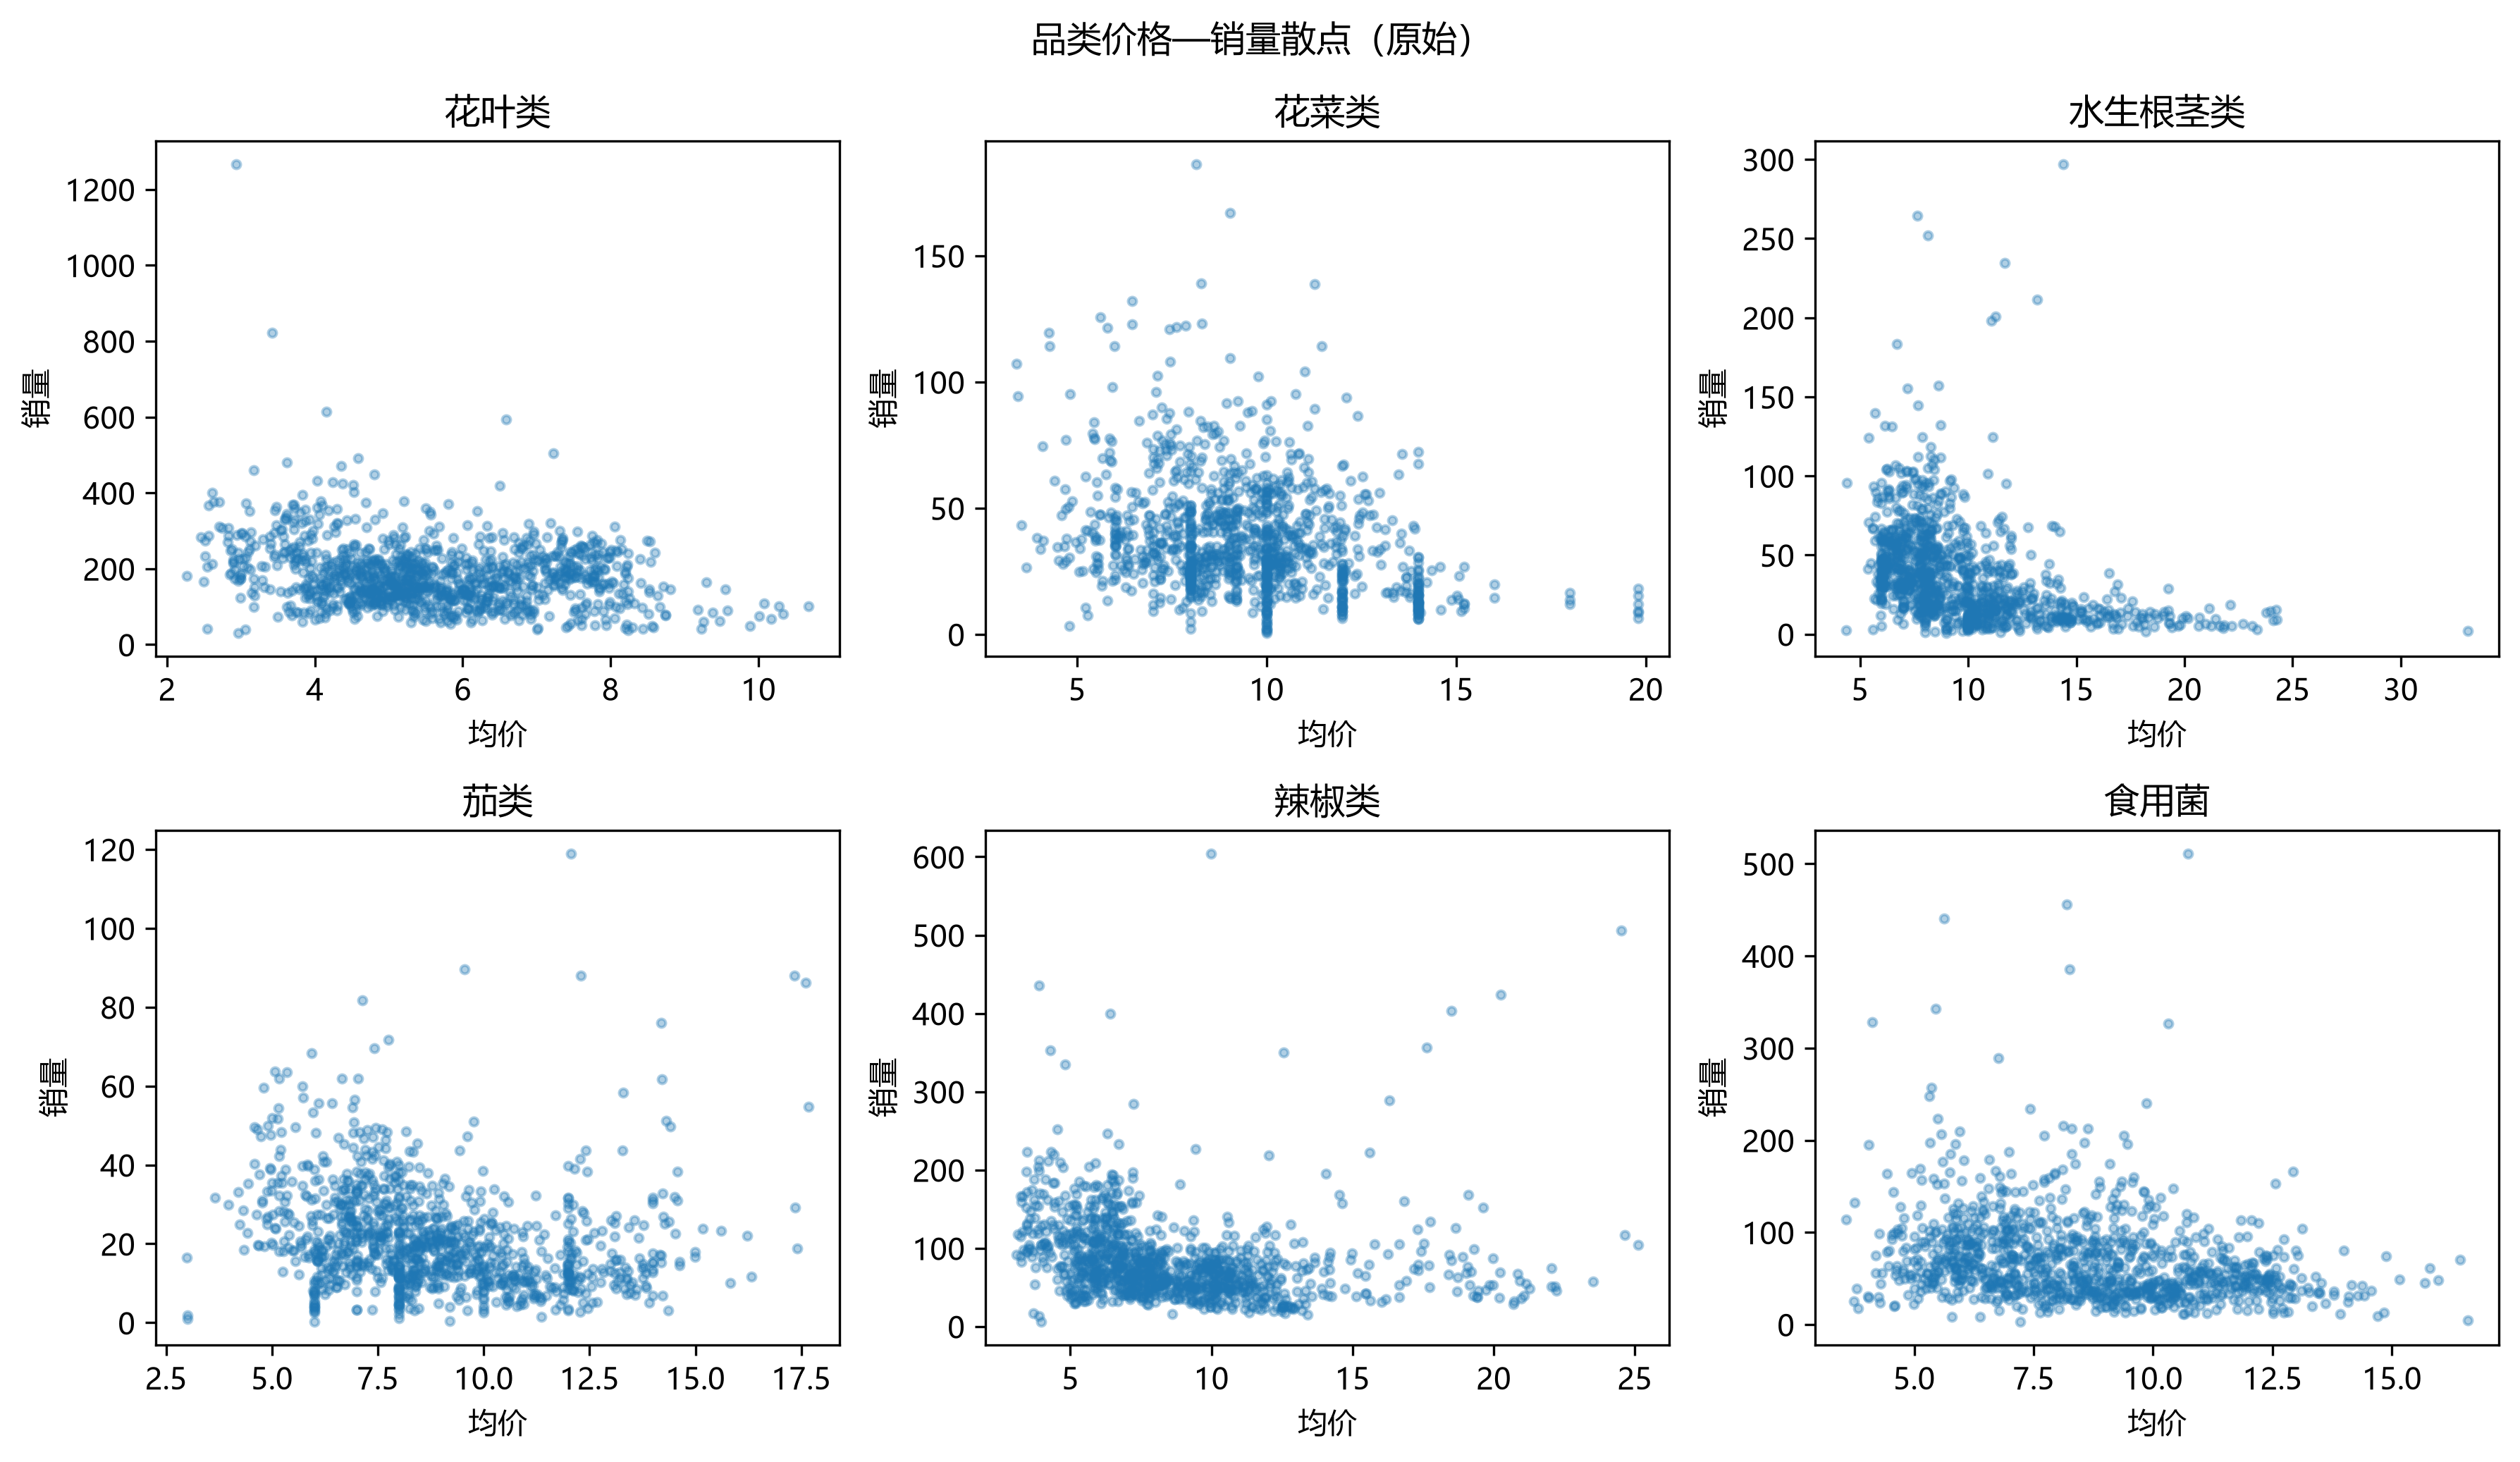
\includegraphics[width=0.95\textwidth]{figures/q2_price_qty_scatter.png}
\caption{价格—销量散点}
\label{fig:scatter}
\end{figure}

\begin{figure}[H]
\centering
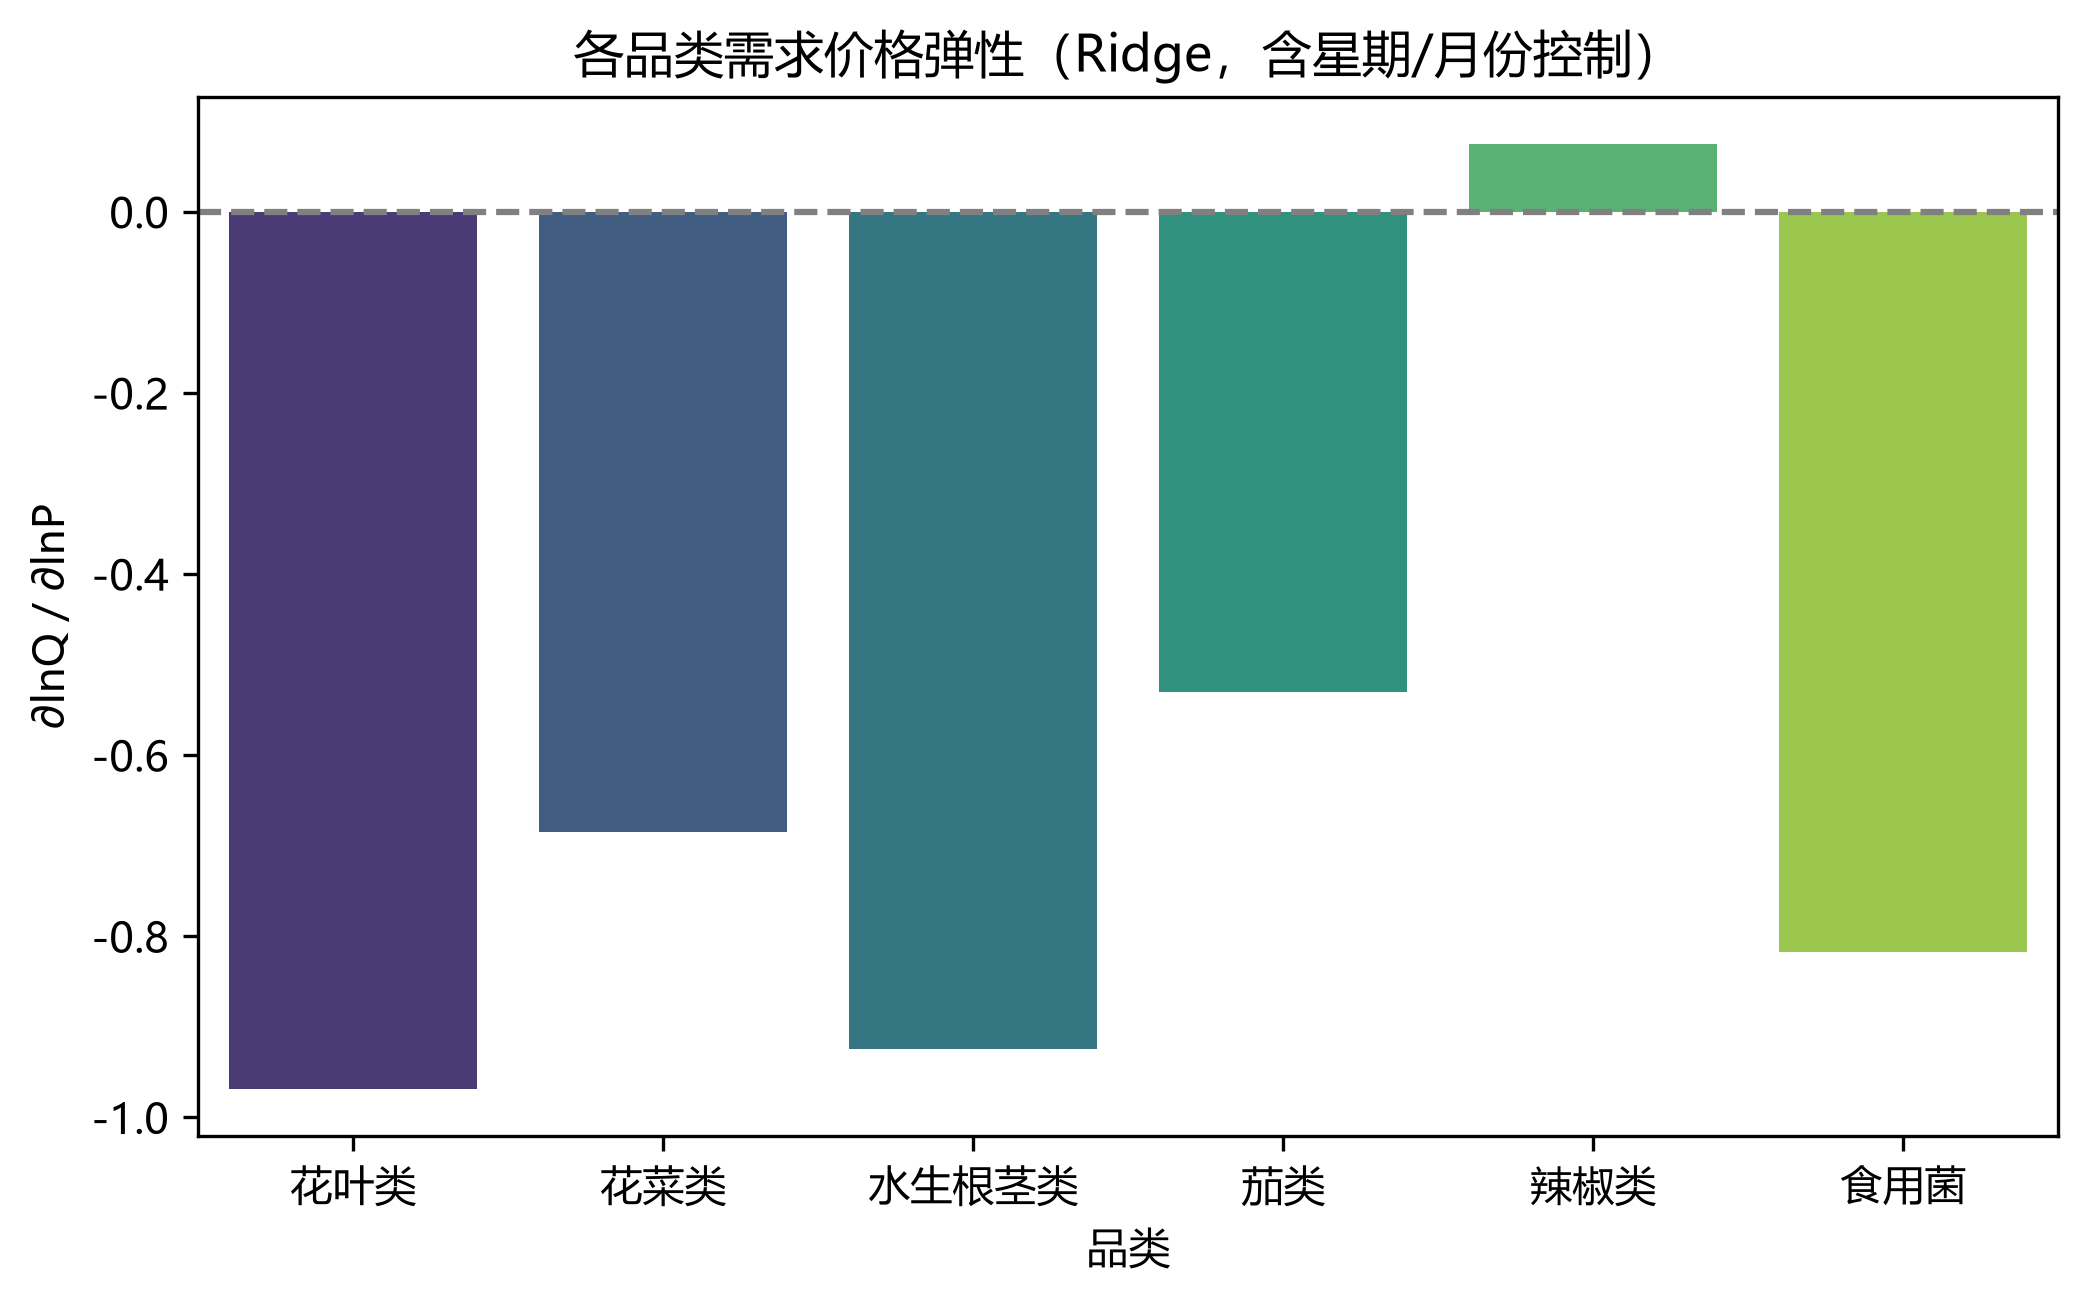
\includegraphics[width=0.85\textwidth]{figures/q2_elasticity.png}
\caption{品类价格弹性}
\label{fig:elast}
\end{figure}

\begin{table}[H]
\centering
\caption{弹性估计与预测检验}
\label{tab:elast}
\scriptsize
\begin{tabular}{lcccc}
\toprule
品类 & 价格弹性 & 时序CV-MAE & 相对均值基线提升 & 历史平均加成率 \\
\hline
花叶类 & -0.97 & 61.32 & -0.00 & 0.67 \\
花菜类 & -0.69 & 16.41 & 0.03 & 0.54 \\
水生根茎类 & -0.92 & 18.96 & 0.16 & 0.47 \\
茄类 & -0.53 & 8.18 & 0.16 & 0.59 \\
辣椒类 & 0.07 & 38.04 & -0.07 & 0.64 \\
食用菌 & -0.82 & 34.91 & -0.05 & 0.58 \\
\bottomrule
\end{tabular}
\end{table}

\begin{figure}[H]
\centering
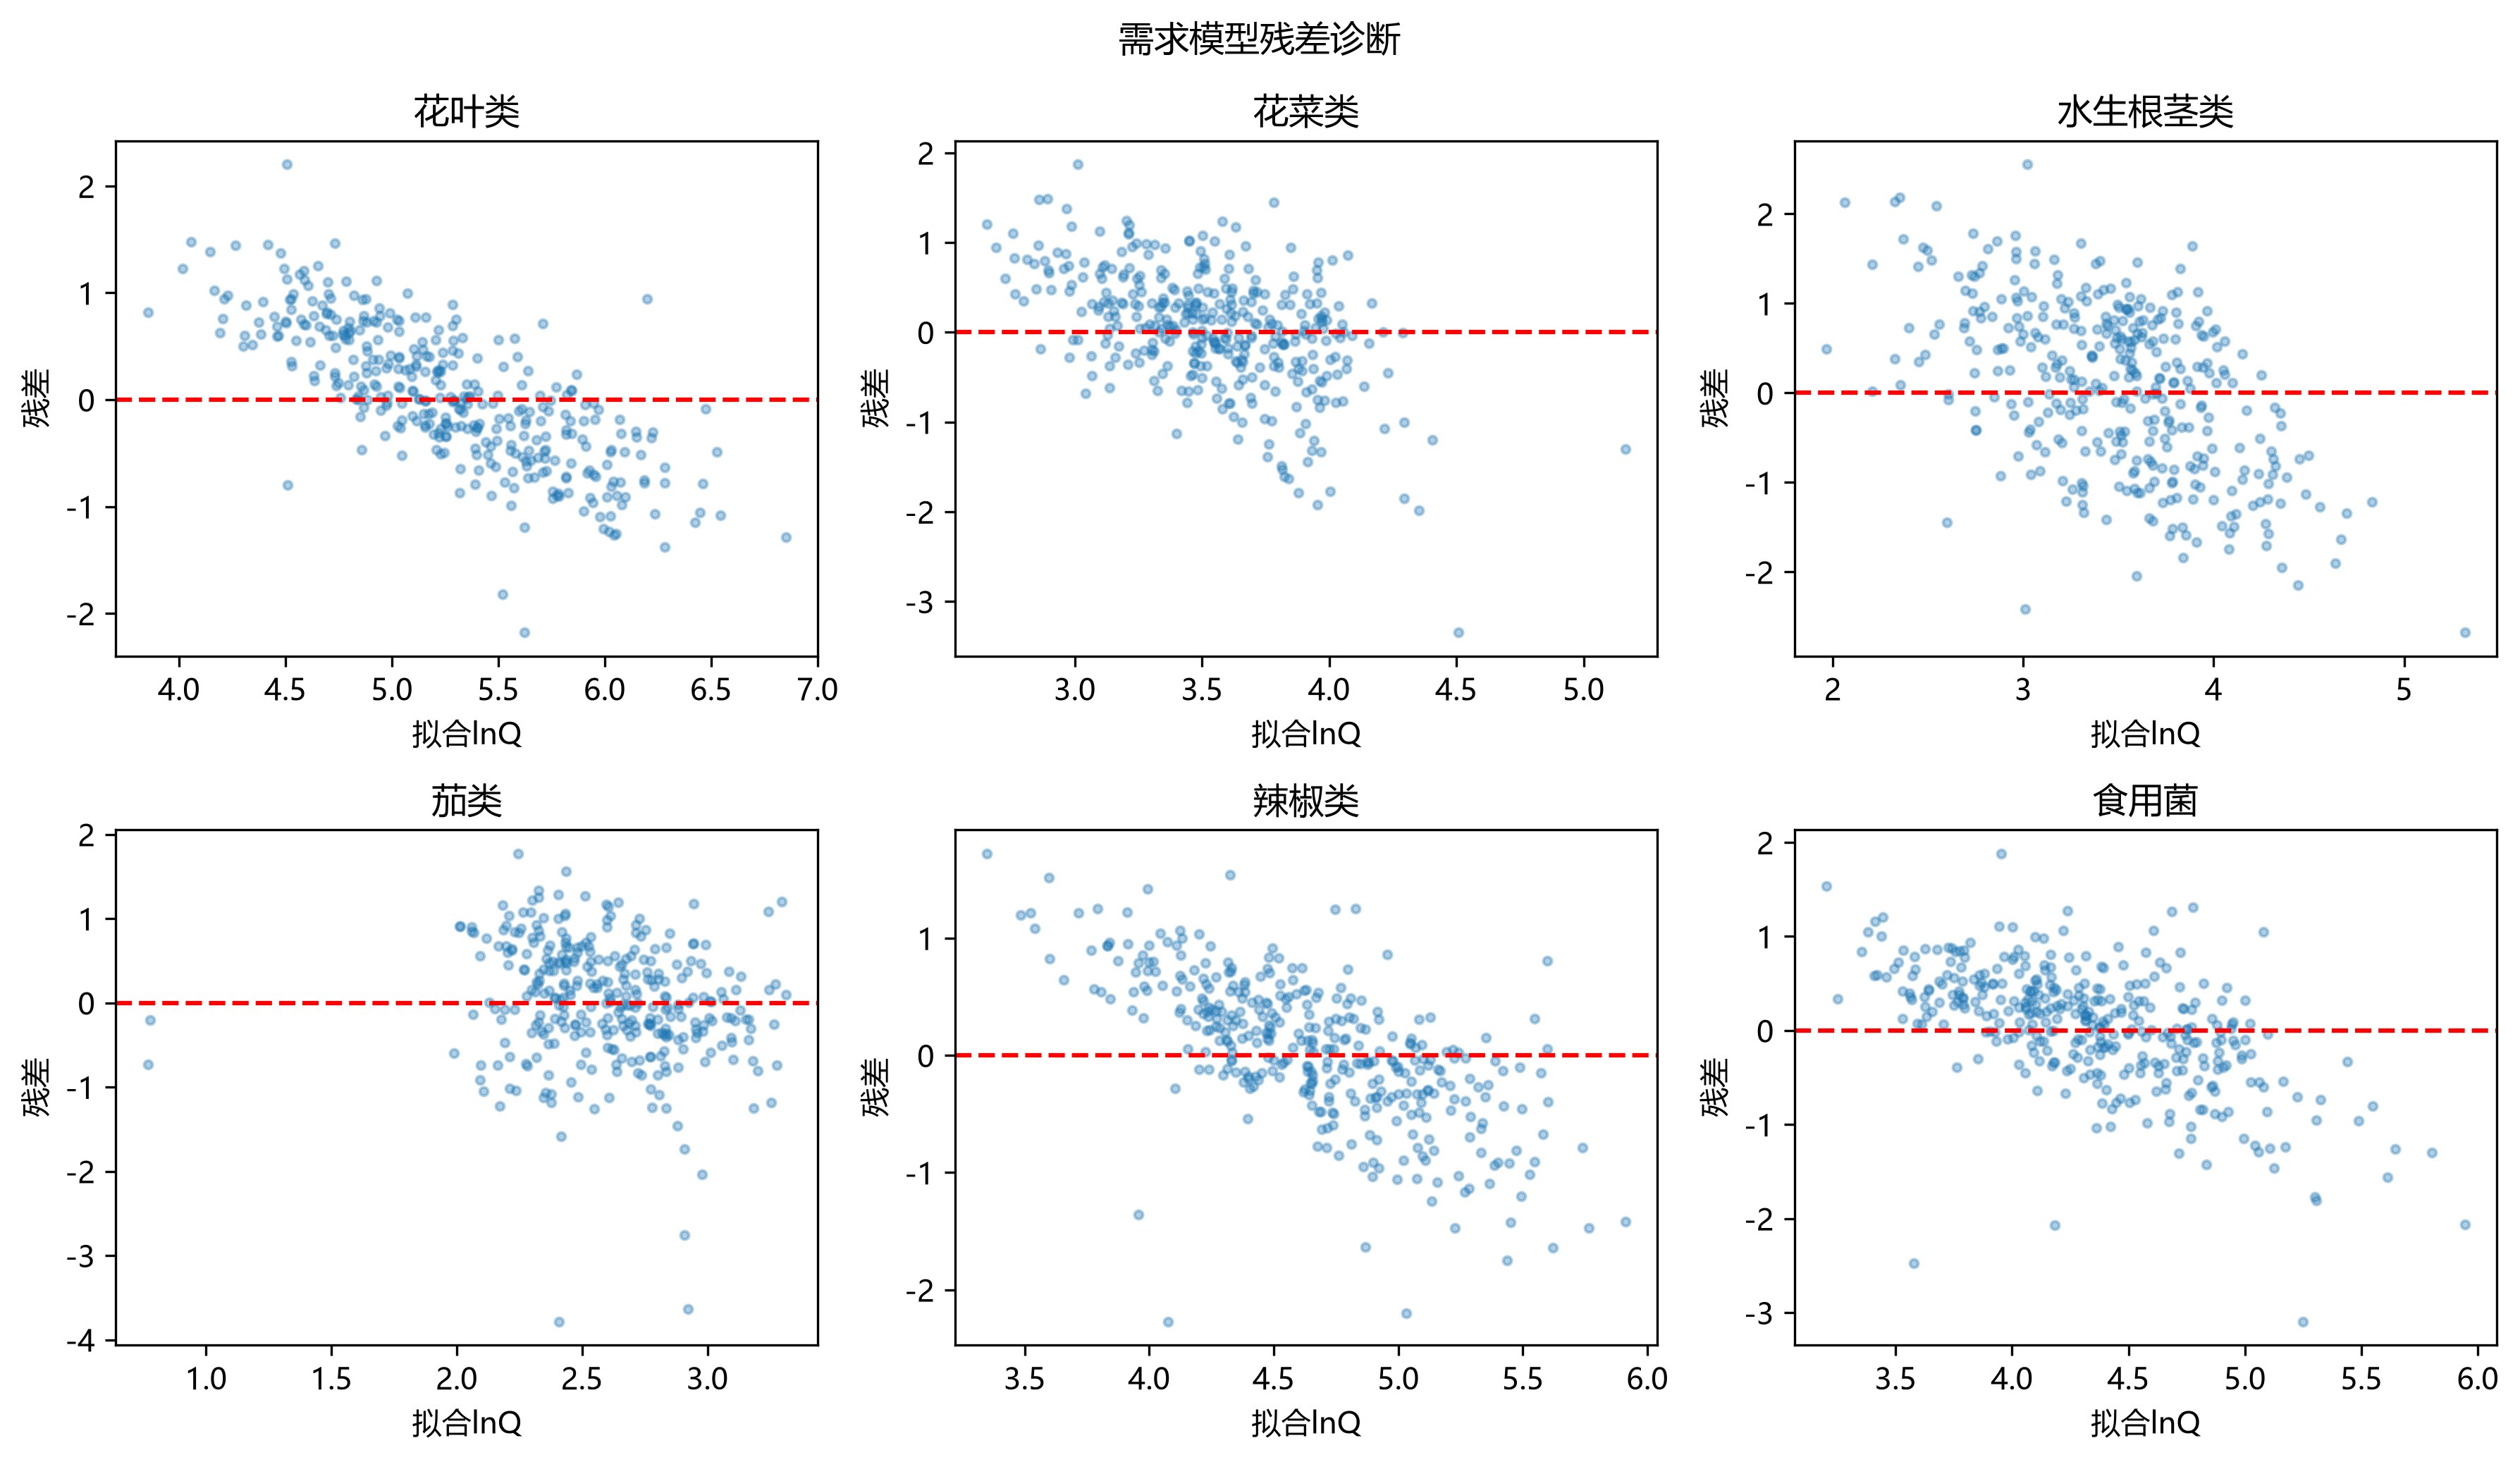
\includegraphics[width=0.95\textwidth]{figures/q2_residual_diagnostics.png}
\caption{需求模型残差诊断}
\label{fig:resid}
\end{figure}

\subsection{收益模型与算法}
设损耗率$\ell_i$，若按需求匹配补货，则
\begin{align}
R_{it}&=\frac{q_{it}(p_{it})}{1-\ell_i},\\
\pi_{it}&=p_{it}q_{it}(p_{it})-c_{it}R_{it}
=\left(p_{it}-\frac{c_{it}}{1-\ell_i}\right)q_{it}(p_{it}).
\end{align}
定价采用成本加成$p=c(1+r)$，对$r$在合理区间网格搜索：

\begin{algorithm}[H]
\caption{品类日度加成率优化}
\begin{algorithmic}[1]
\For{each category $i$, day $t$}
\State 预测批发价$c_{it}$，读取损耗$\ell_i$
\For{$r$ in grid}
\State $p\leftarrow c(1+r)$，预测$q(p)$
\State $R\leftarrow q/(1-\ell)$，计算$\pi(r)$
\EndFor
\State 取$\hat r=\arg\max \pi(r)$，输出$(R,p)$
\EndFor
\end{algorithmic}
\end{algorithm}

\subsection{结果}
周计划汇总见表~\ref{tab:q2}与表~\ref{tab:day}，补货堆叠图、售价路径与收益见图~\ref{fig:repl}--\ref{fig:catprofit}。加成--收益曲线见图~\ref{fig:curve}。主模型周收益\textbf{6655.06}元，周补货\textbf{2606.40}kg，平均加成\textbf{80.65\%}；相对历史加成提升\textbf{54.93\%}，相对固定30\%加成提升\textbf{239.54\%}。

\begin{table}[H]
\centering
\caption{未来一周品类策略汇总}
\label{tab:q2}
\scriptsize
\begin{tabular}{lccccc}
\toprule
品类 & 周补货总量 & 周预期销量 & 周收益 & 平均加成率 & 平均售价 \\
\hline
花叶类 & 1070.45 & 933.11 & 2218.74 & 0.87 & 6.17 \\
花菜类 & 151.91 & 128.35 & 620.80 & 0.72 & 15.43 \\
水生根茎类 & 79.00 & 68.21 & 464.13 & 0.70 & 21.44 \\
茄类 & 175.35 & 163.64 & 563.88 & 0.82 & 8.38 \\
辣椒类 & 694.13 & 629.99 & 1844.08 & 0.99 & 6.58 \\
食用菌 & 435.57 & 394.41 & 943.43 & 0.75 & 6.50 \\
\bottomrule
\end{tabular}
\end{table}

\begin{table}[H]
\centering
\caption{各日品类补货量（kg）}
\label{tab:day}
\scriptsize
\begin{tabular}{lcccccc}
\toprule
日期 & 水生根茎类 & 花叶类 & 花菜类 & 茄类 & 辣椒类 & 食用菌 \\
\hline
07-01 & 15.80 & 193.27 & 30.14 & 34.21 & 138.09 & 89.91 \\
07-02 & 15.84 & 206.78 & 27.21 & 39.38 & 133.73 & 91.24 \\
07-03 & 8.25 & 139.86 & 17.08 & 22.21 & 84.67 & 51.53 \\
07-04 & 9.58 & 145.23 & 20.11 & 19.48 & 88.24 & 47.84 \\
07-05 & 9.21 & 130.79 & 16.64 & 18.24 & 75.31 & 51.43 \\
07-06 & 7.74 & 117.01 & 19.30 & 18.86 & 83.65 & 47.62 \\
07-07 & 12.57 & 137.51 & 21.43 & 22.97 & 90.43 & 55.99 \\
\bottomrule
\end{tabular}
\end{table}

\begin{figure}[H]
\centering
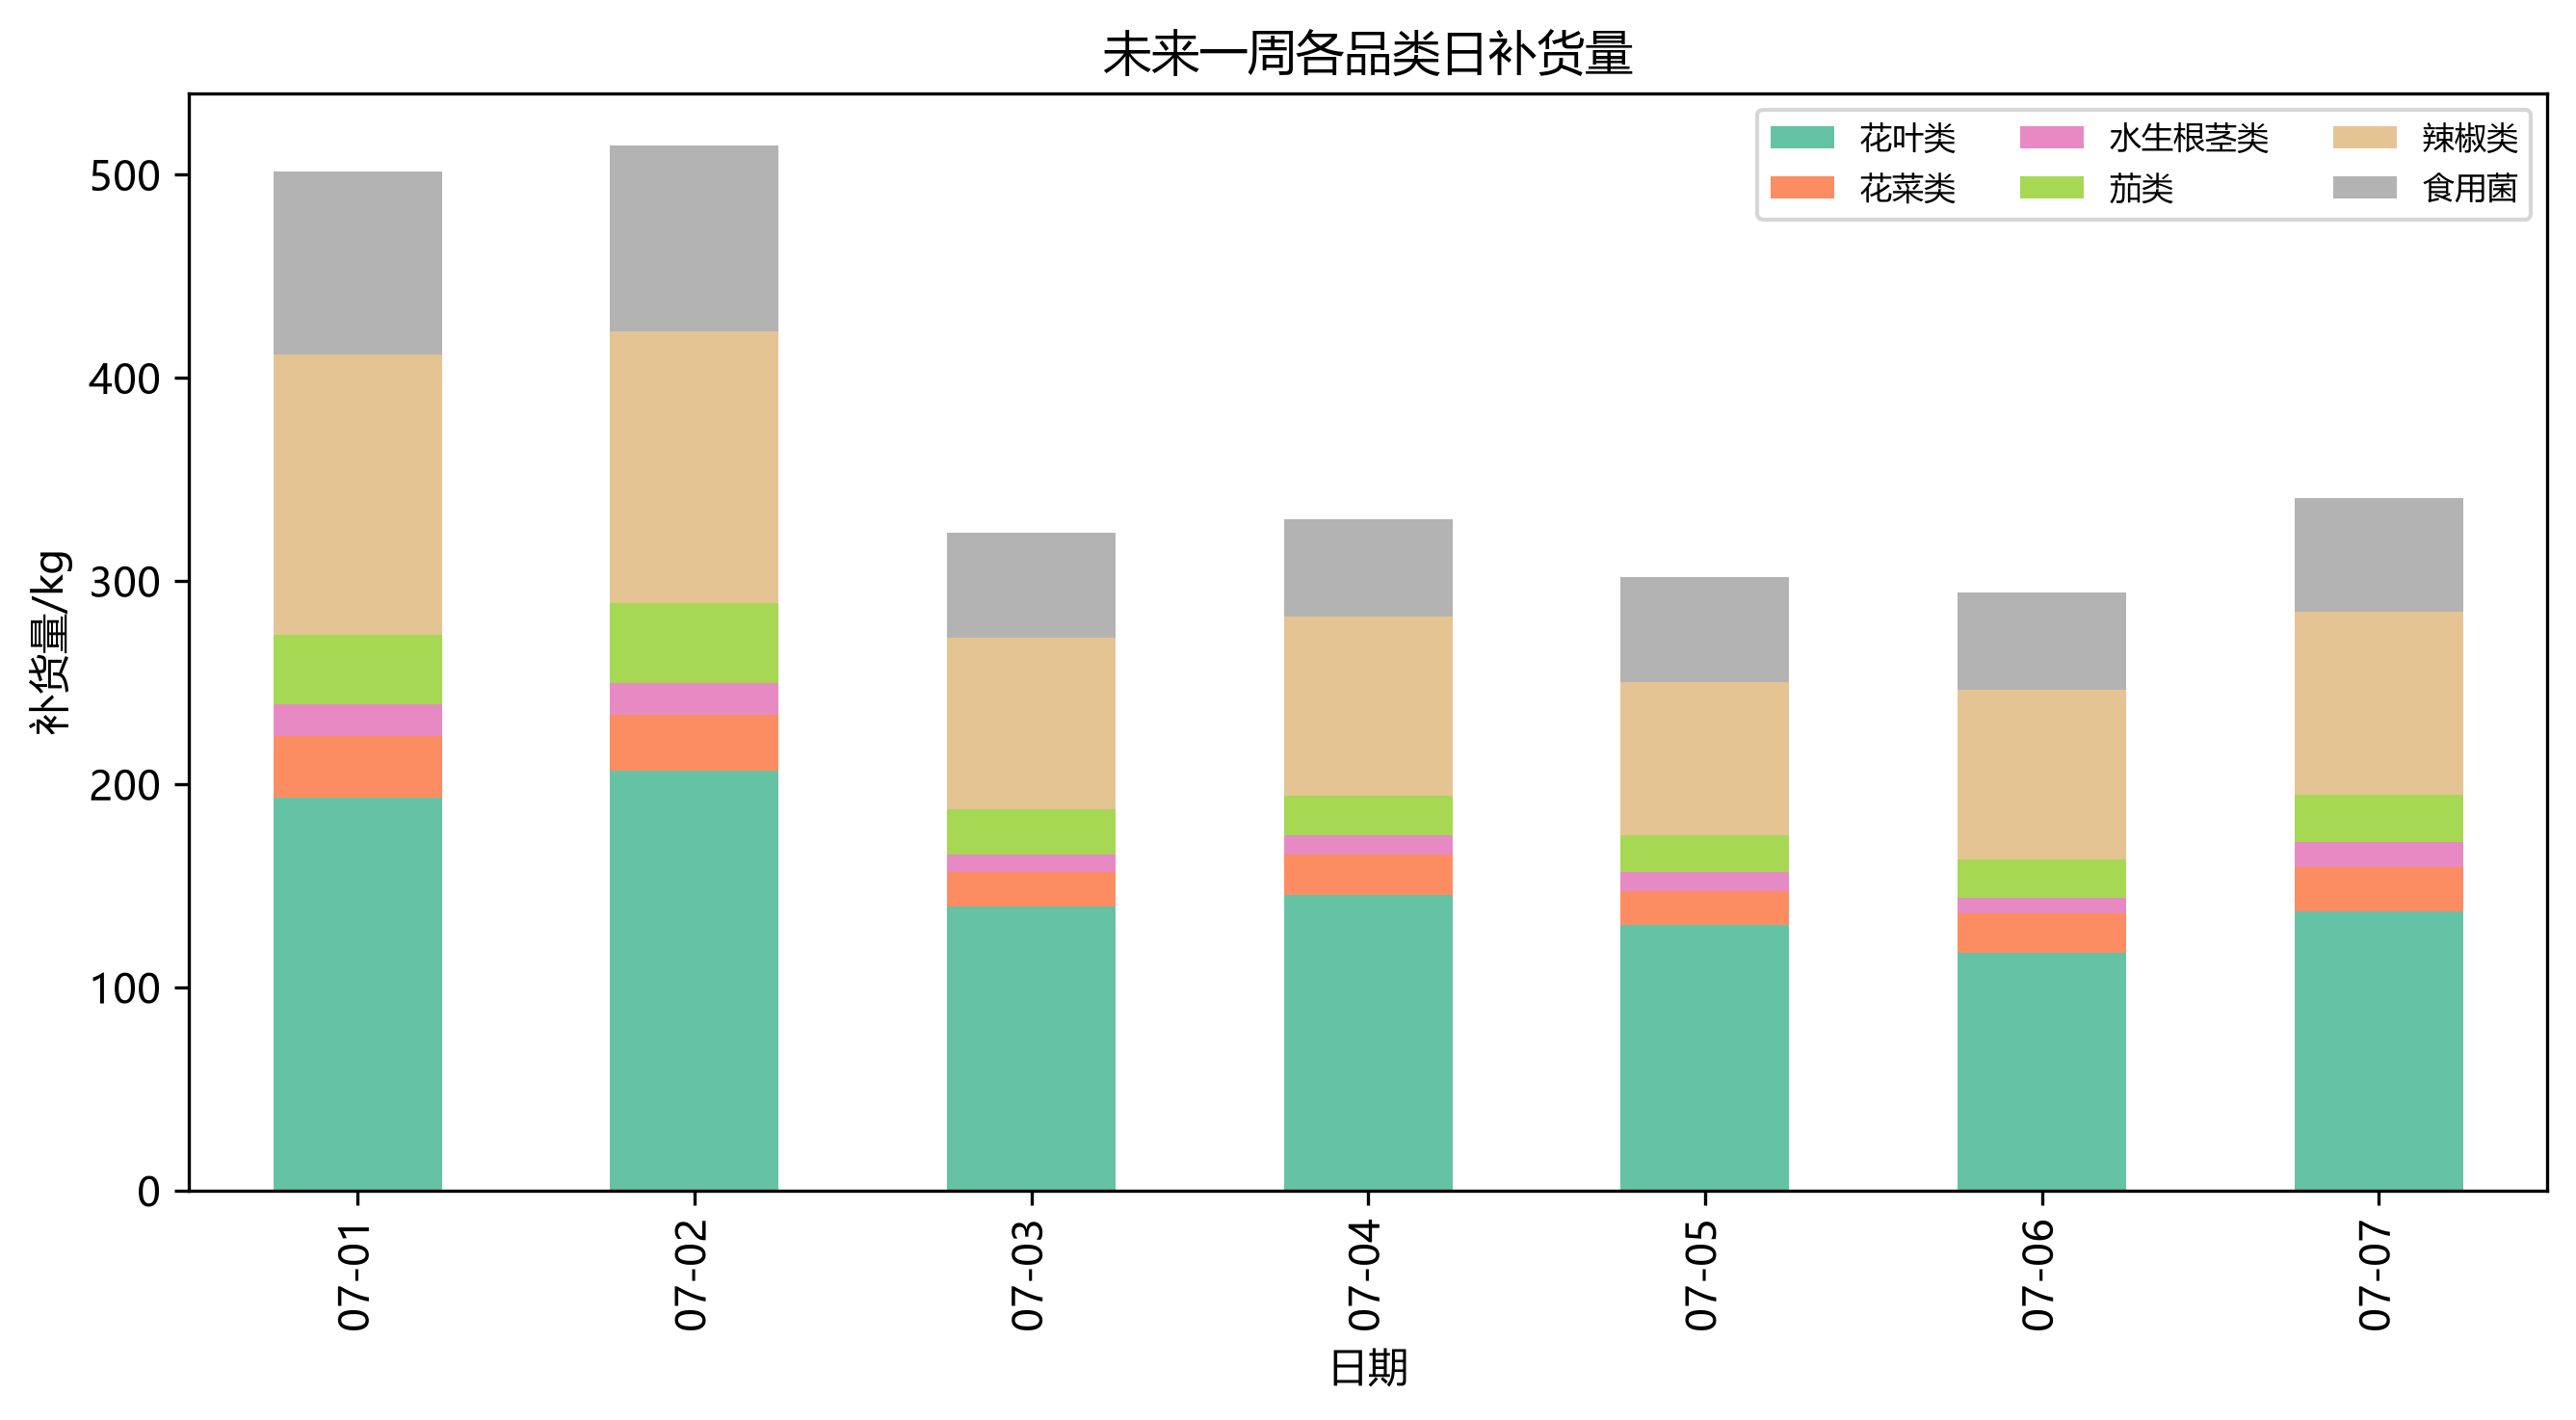
\includegraphics[width=0.95\textwidth]{figures/q2_replenish_stacked.png}
\caption{一周补货量堆叠图}
\label{fig:repl}
\end{figure}

\begin{figure}[H]
\centering
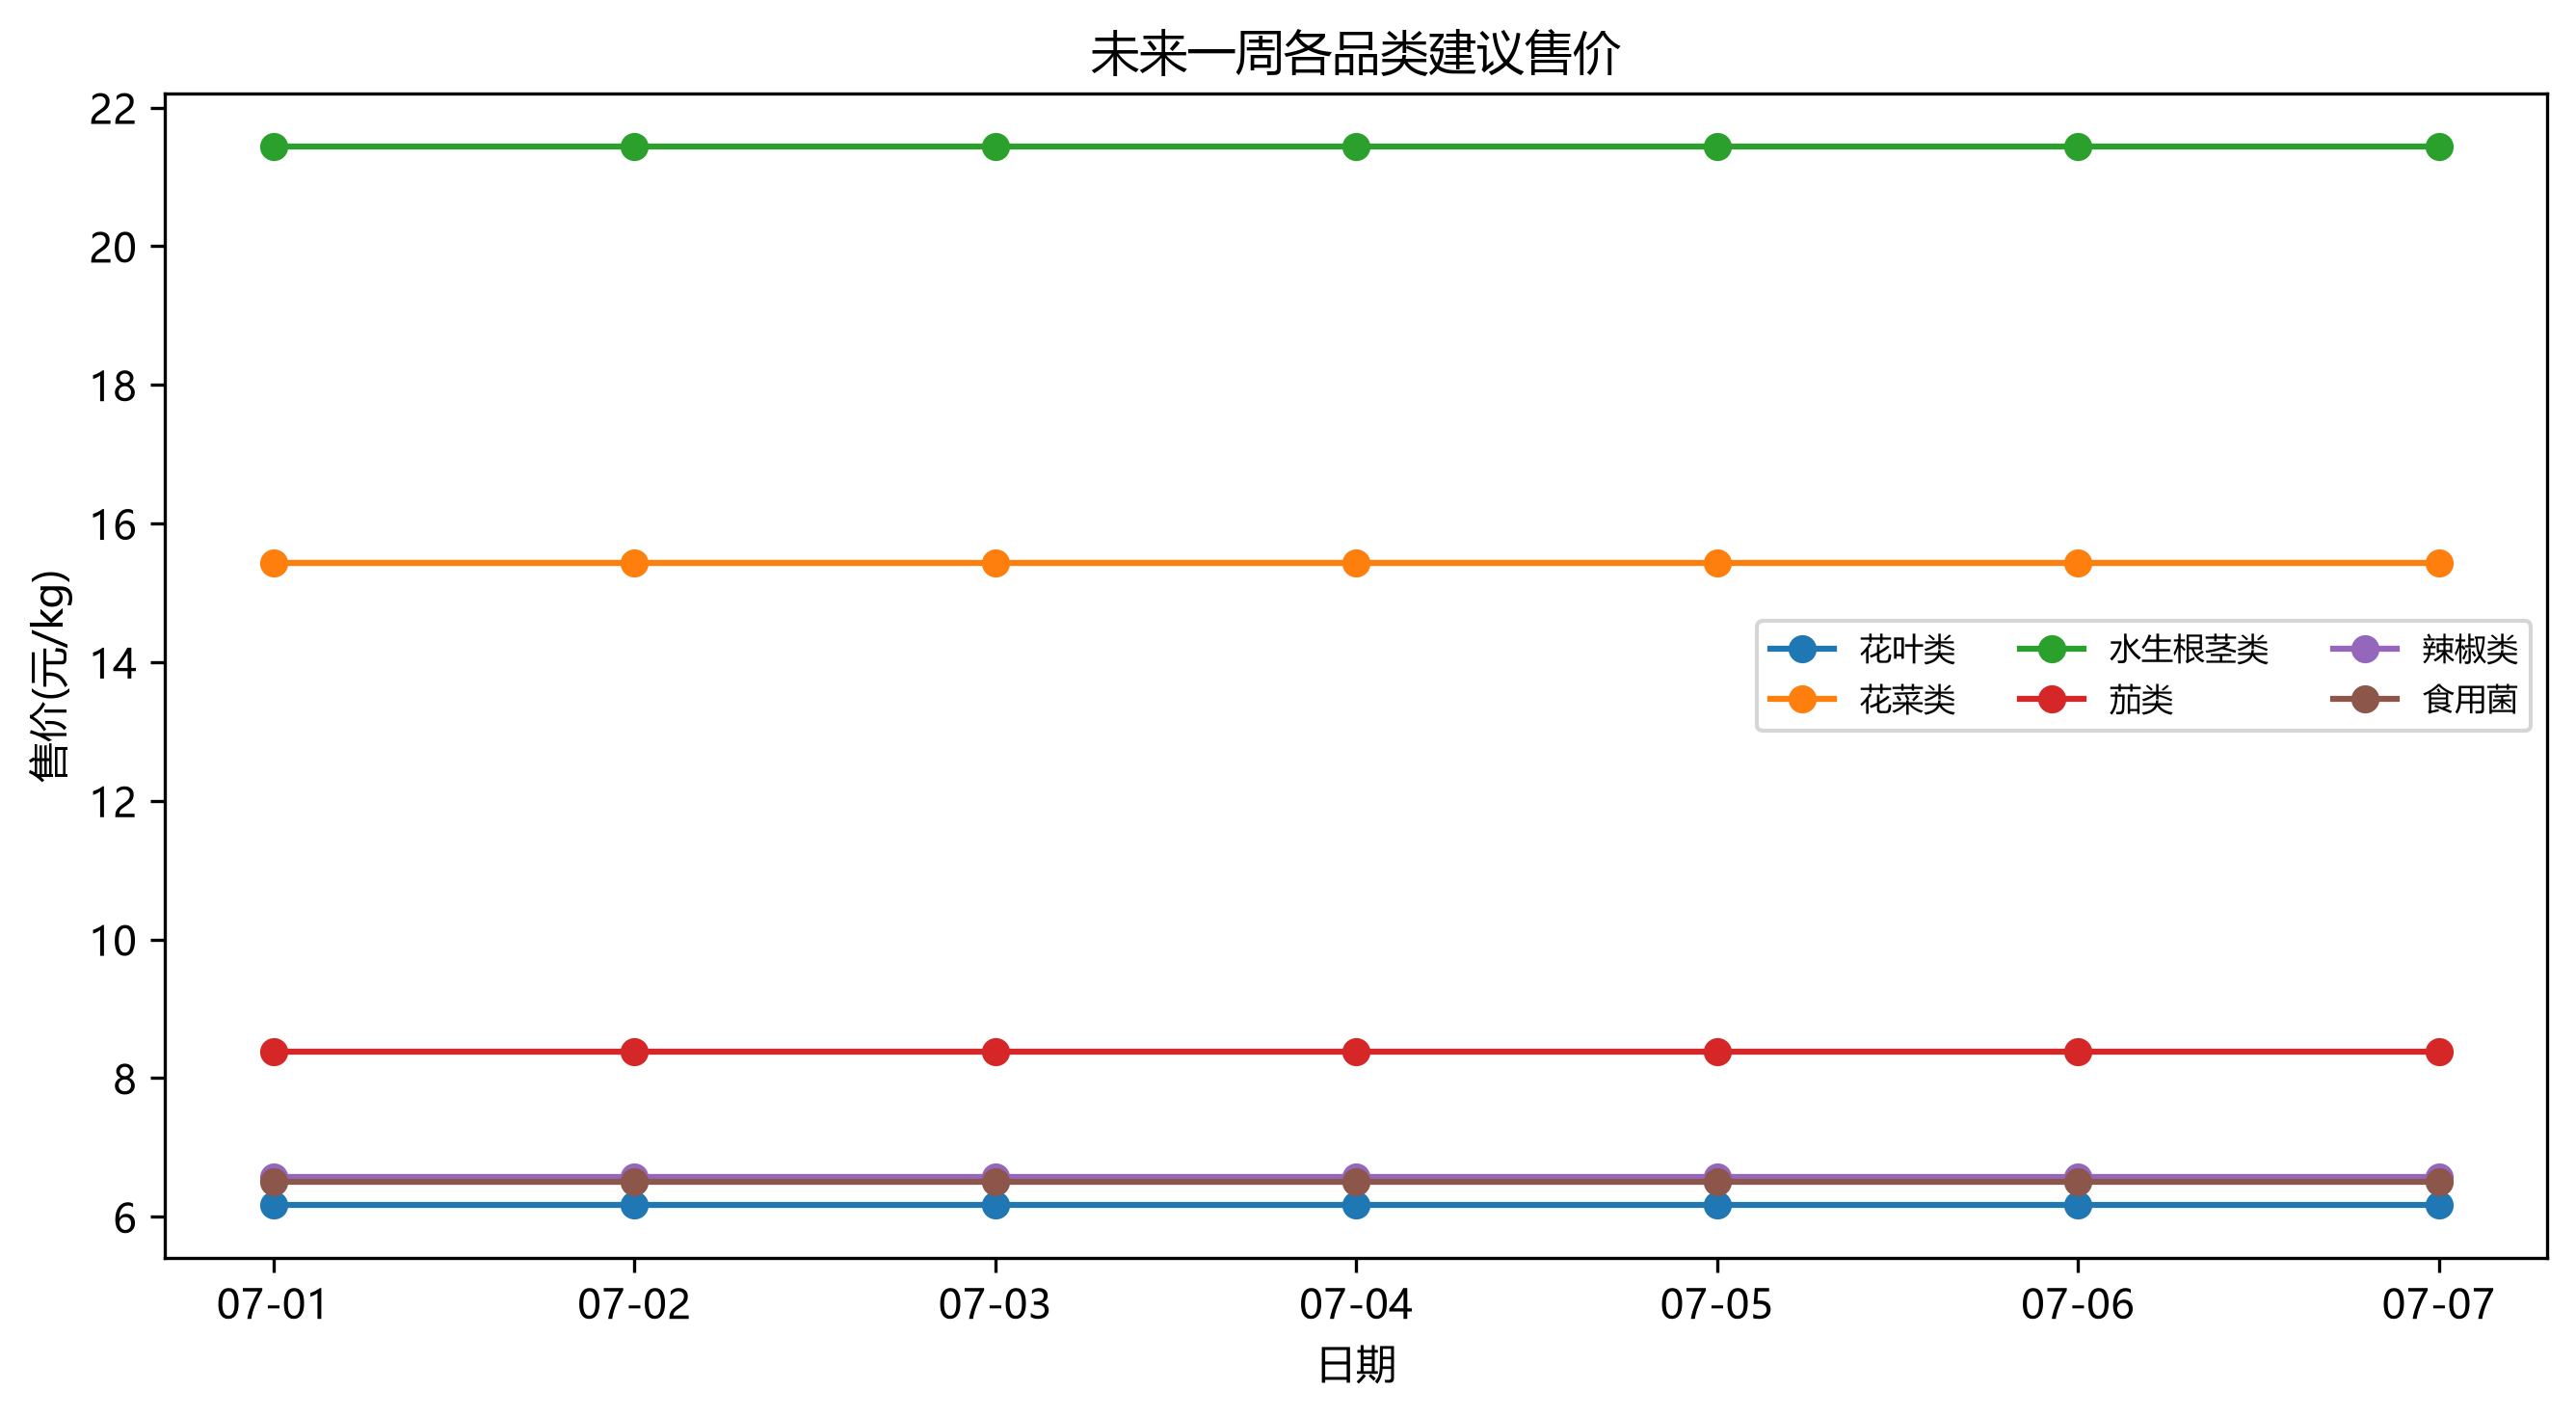
\includegraphics[width=0.95\textwidth]{figures/q2_price_strategy.png}
\caption{一周售价策略}
\label{fig:price}
\end{figure}

\begin{figure}[H]
\centering
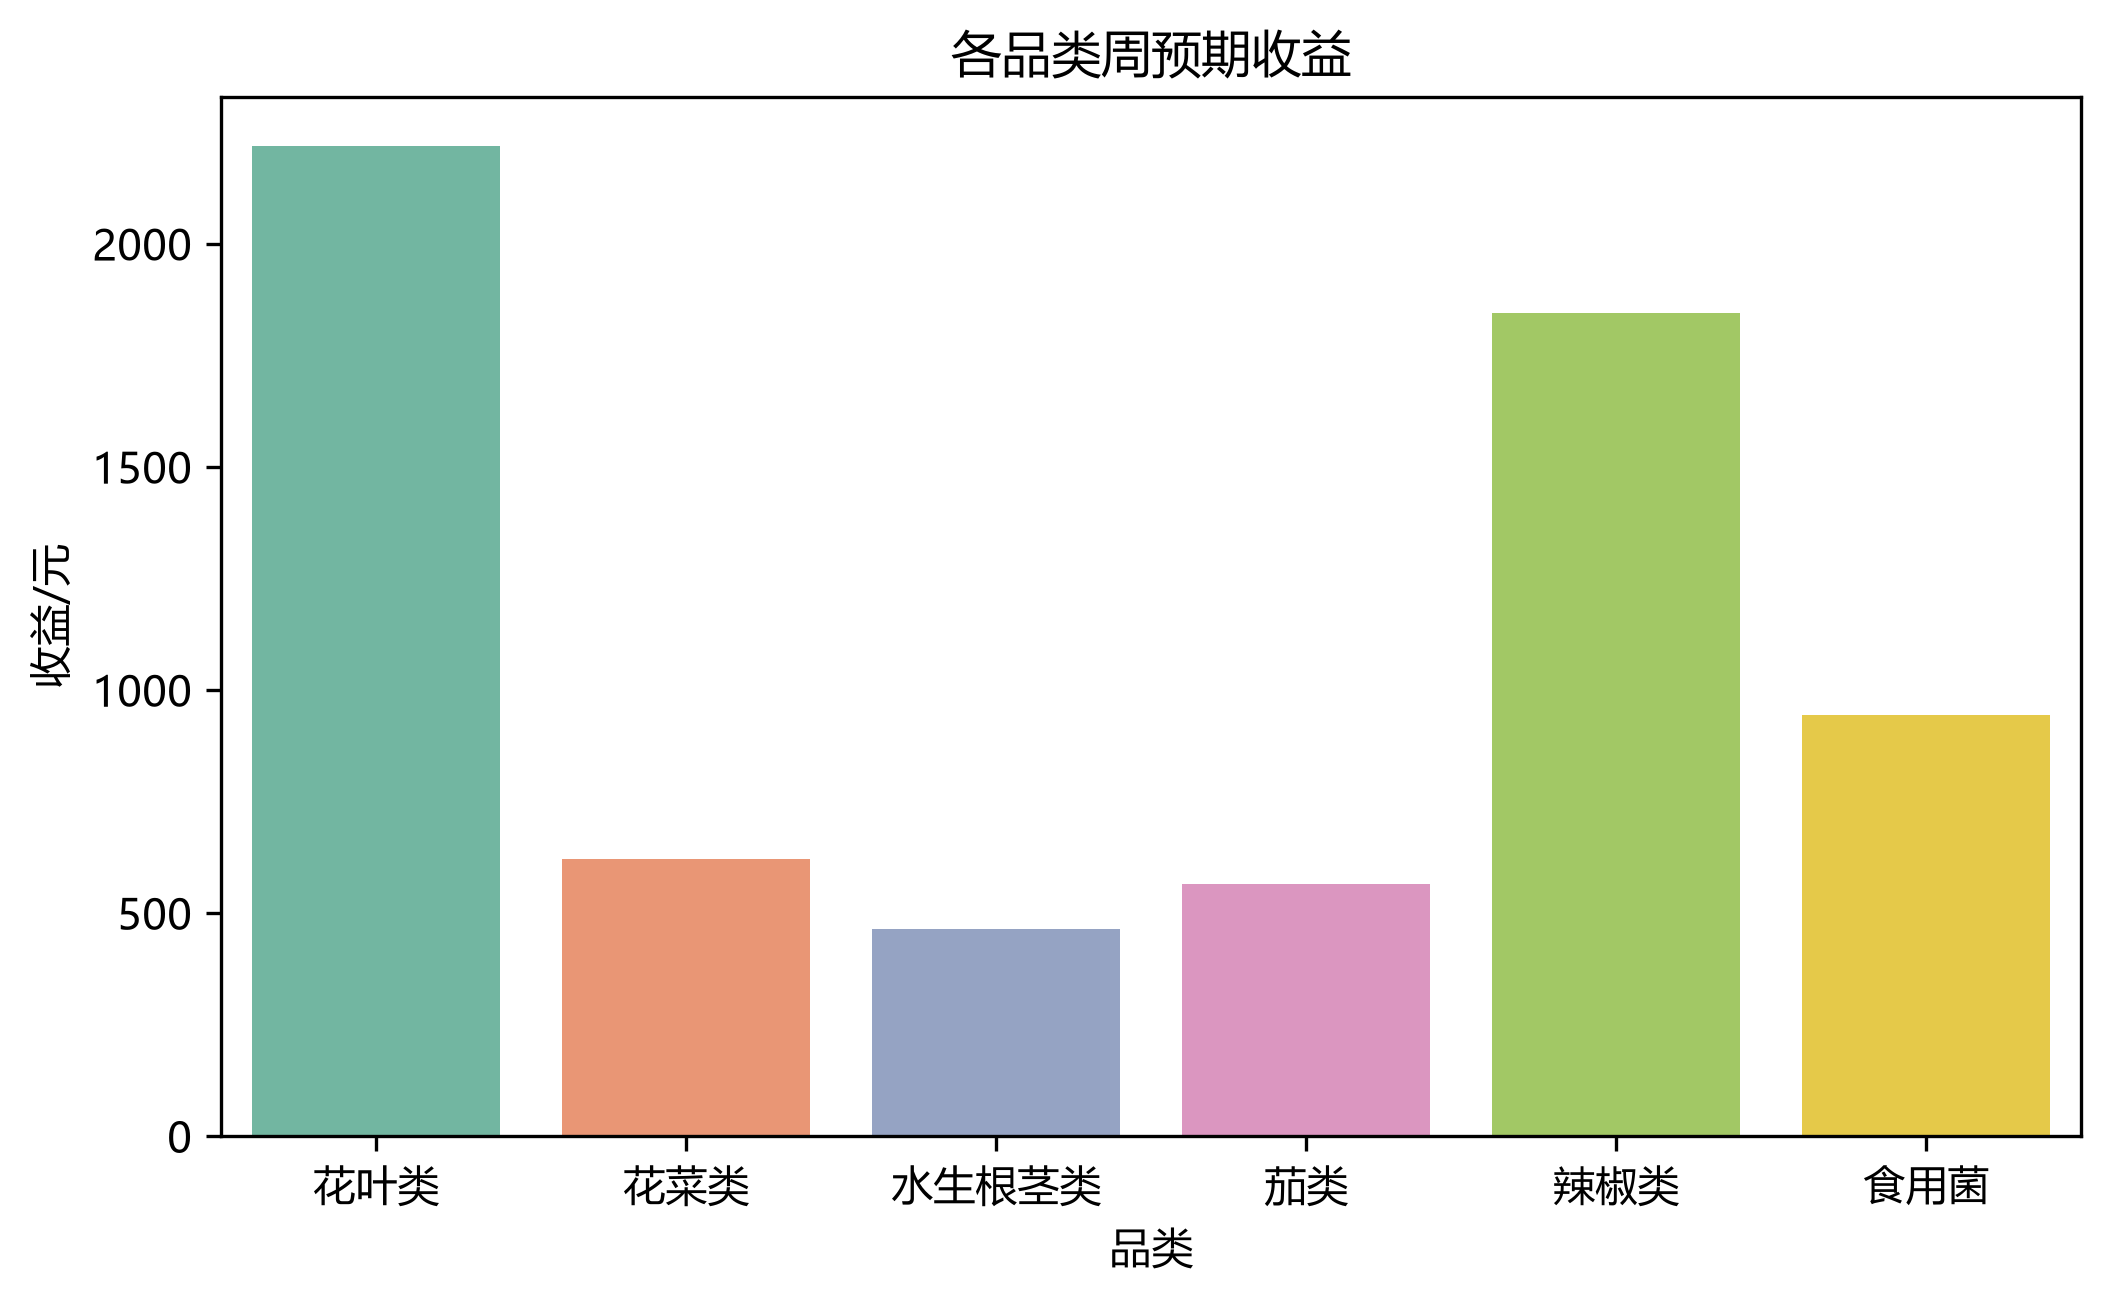
\includegraphics[width=0.85\textwidth]{figures/q2_category_profit.png}
\caption{品类周收益}
\label{fig:catprofit}
\end{figure}

\begin{figure}[H]
\centering
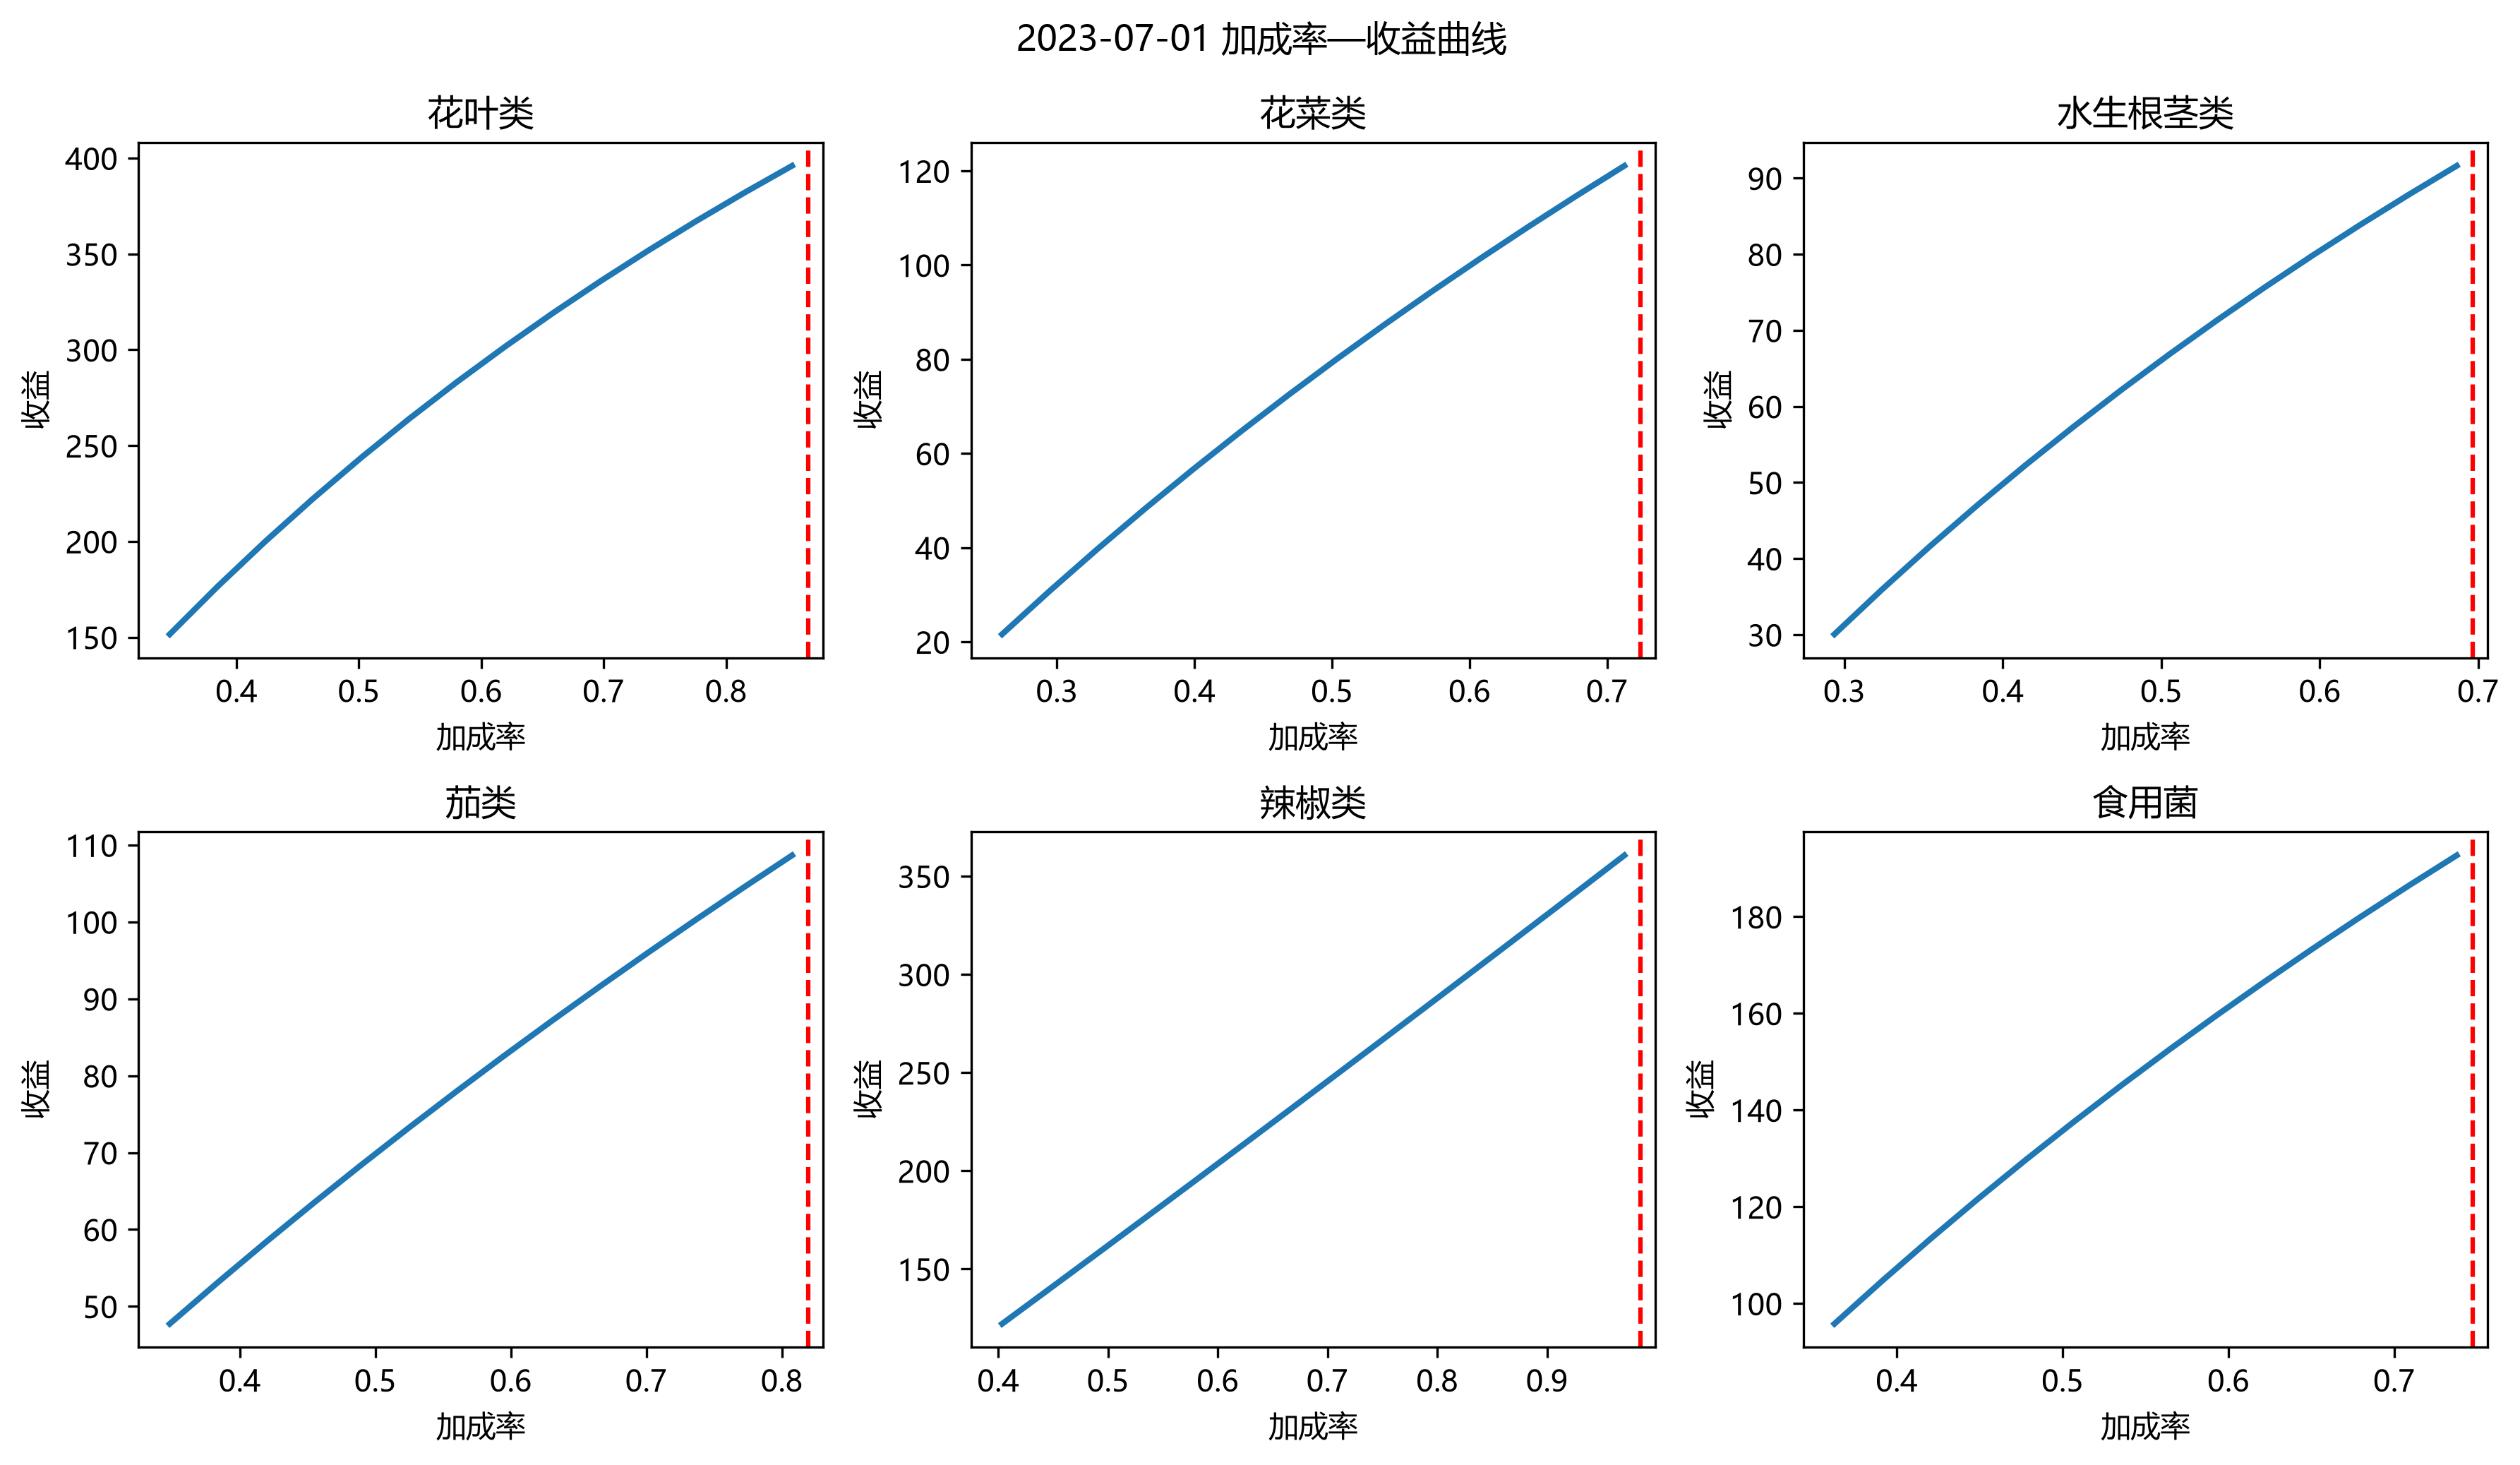
\includegraphics[width=0.95\textwidth]{figures/q2_markup_profit_curve.png}
\caption{加成率—收益曲线（7月1日）}
\label{fig:curve}
\end{figure}

\subsection{结果解读与实施要点}
\begin{enumerate}[leftmargin=2em]
\item \textbf{结构贡献}：花叶类与辣椒类贡献主要补货量与收益，应优先配置自动调价与晨间补货带宽；水生根茎类单位溢价高但体量小，适合作利润补充。
\item \textbf{弹性含义}：多数品类$\varepsilon\in(-1,0)$，纯利润目标在历史可行域内易靠近加成上界。本文将搜索限制在历史分位带，避免脱离可售现实的``无限提价''。
\item \textbf{损耗杠杆}：由$R=q/(1-\ell)$，损耗低估会系统性抬高收益；盘点质量直接决定模型可信度。
\item \textbf{星期差异}：需求按``同星期近期销量''标定，一周补货随工作日/周末客流变化，而非简单复制同一天计划。
\end{enumerate}

\subsection{与下一问衔接}
Q2给出品类层``需求目标+价格机制''。Q3将在货架容量约束下选择单品，使品类需求尽量被覆盖的同时最大化收益。

\section{问题3：单品补货与定价}
\subsection{问题定位}
基于2023-06-24至06-30可售集合，选择27--33个单品，满足最小陈列2.5\,kg，尽量满足品类需求并最大化7月1日收益。

\subsection{模型}
对候选单品$j$，以历史中位销量$q_j^0$与均价$p_j^0$为锚，结合弹性$\varepsilon_j$：
\begin{equation}
q_j(p)=q_j^0\left(\frac{p}{p_j^0}\right)^{\varepsilon_j},\quad
p=c_j(1+r).
\end{equation}
补货
\begin{equation}
R_j=\max\left\{2.5,\ \frac{q_j(p)}{1-\ell_j}\right\},
\quad
\pi_j=p\cdot\min\{q_j,R_j(1-\ell_j)\}-c_j R_j.
\end{equation}
整数规划\cite{mip}：
\begin{align}
\max_{x_j\in\{0,1\}}\quad &
\sum_j \pi_j x_j-\lambda \bar m\sum_{k}\mathrm{unmet}_k \\
\mathrm{s.t.}\quad &
27\le \sum_j x_j\le 33,\\
& \mathrm{unmet}_k \ge D_k-\sum_{j\in k} q_j x_j,\\
& \sum_{j\in k}x_j\ge 1\quad(\text{有候选时}),\\
& R_j\ge 2.5\quad(\text{入选后}).
\end{align}

\subsection{结果与对照}
求解得到入选\textbf{33}个单品，预期收益\textbf{1446.34}元，补货\textbf{365.95}kg，相对贪心Top收益提升\textbf{3.64\%}。方法对比见表~\ref{tab:q3cmp}与图~\ref{fig:q3cmp}，品类覆盖见表~\ref{tab:cov}与图~\ref{fig:cov}，入选清单见表~\ref{tab:plan3}与图~\ref{fig:sku}。

\subsection{组合结构解读}
ILP相对贪心Top收益的增益虽然绝对比例不高，但关键在于\textbf{约束可行且品类覆盖完整}：随机30常出现品类缺失，纯销量Top则可能挤出高毛利但销量中等的单品。入选结果中，花叶类单品数最多，与其需求体量匹配；花菜类、茄类以少量高贡献单品完成覆盖，体现``少而精''；辣椒类与食用菌兼顾份装与散称，有利于满足最小陈列并控制损耗。

对门店执行，建议把表~\ref{tab:plan3}转化为晨间订货单：先锁定名额内单品集合，再按补货量下单；售价按建议加成写入电子价签，并保留人工可调的安全区间（例如$\pm 5\%$），以吸收批发价临时波动。

\begin{table}[H]
\centering
\caption{单品方案方法对比}
\label{tab:q3cmp}
\begin{tabular}{lccccc}
\toprule
方案 & 单品数 & 总补货量 & 总预期销量 & 总收益 & 品类覆盖数 \\
\hline
ILP优化(主模型) & 33 & 365.95 & 333.47 & 1446.34 & 6 \\
贪心Top收益(基线) & 30 & 357.71 & 327.17 & 1395.58 & 6 \\
贪心Top销量(基线) & 30 & 361.18 & 331.40 & 1385.07 & 6 \\
随机30(基线) & 30 & 272.83 & 245.12 & 991.96 & 5 \\
\bottomrule
\end{tabular}
\end{table}

\begin{figure}[H]
\centering
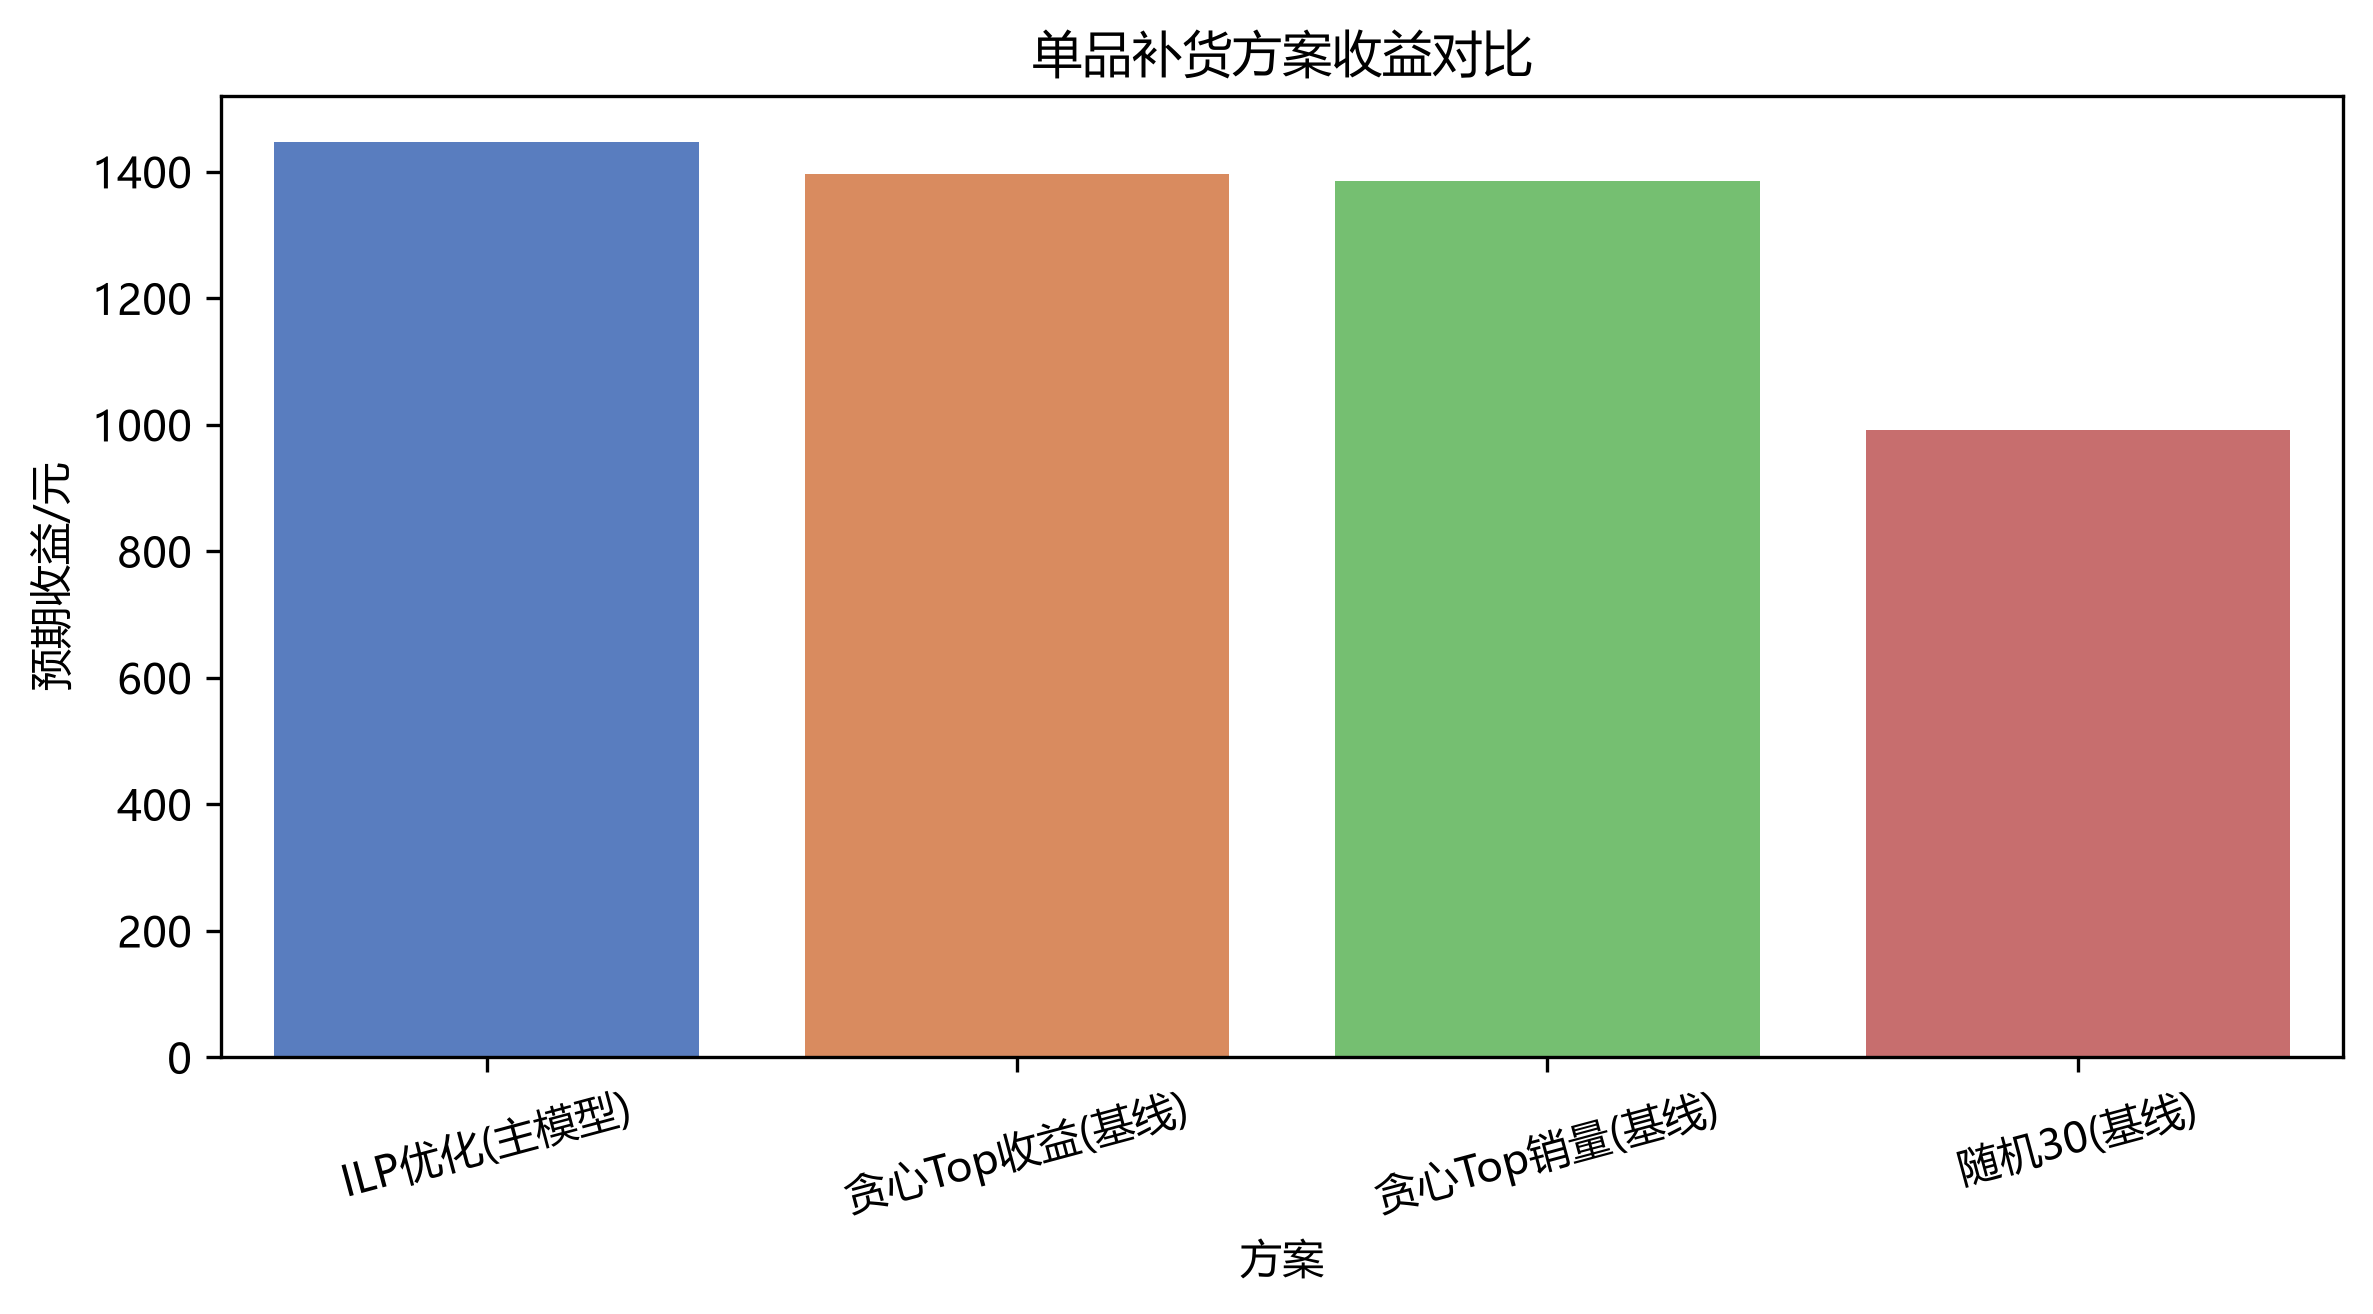
\includegraphics[width=0.85\textwidth]{figures/q3_method_compare.png}
\caption{Q3方法收益对比}
\label{fig:q3cmp}
\end{figure}

\begin{table}[H]
\centering
\caption{品类需求覆盖}
\label{tab:cov}
\scriptsize
\begin{tabular}{lcccccc}
\toprule
分类名称 & 单品数 & 补货量 & 预期销量 & 收益 & 需求目标 & 需求满足率 \\
\hline
花叶类 & 14 & 155.84 & 138.67 & 526.01 & 168.47 & 0.82 \\
花菜类 & 2 & 19.42 & 17.61 & 158.29 & 25.46 & 0.69 \\
水生根茎类 & 3 & 12.85 & 10.78 & 78.71 & 13.65 & 0.79 \\
茄类 & 2 & 26.95 & 25.26 & 141.62 & 31.93 & 0.79 \\
辣椒类 & 8 & 94.10 & 85.09 & 324.01 & 125.33 & 0.68 \\
食用菌 & 4 & 56.78 & 56.06 & 217.69 & 81.41 & 0.69 \\
\bottomrule
\end{tabular}
\end{table}

\begin{figure}[H]
\centering
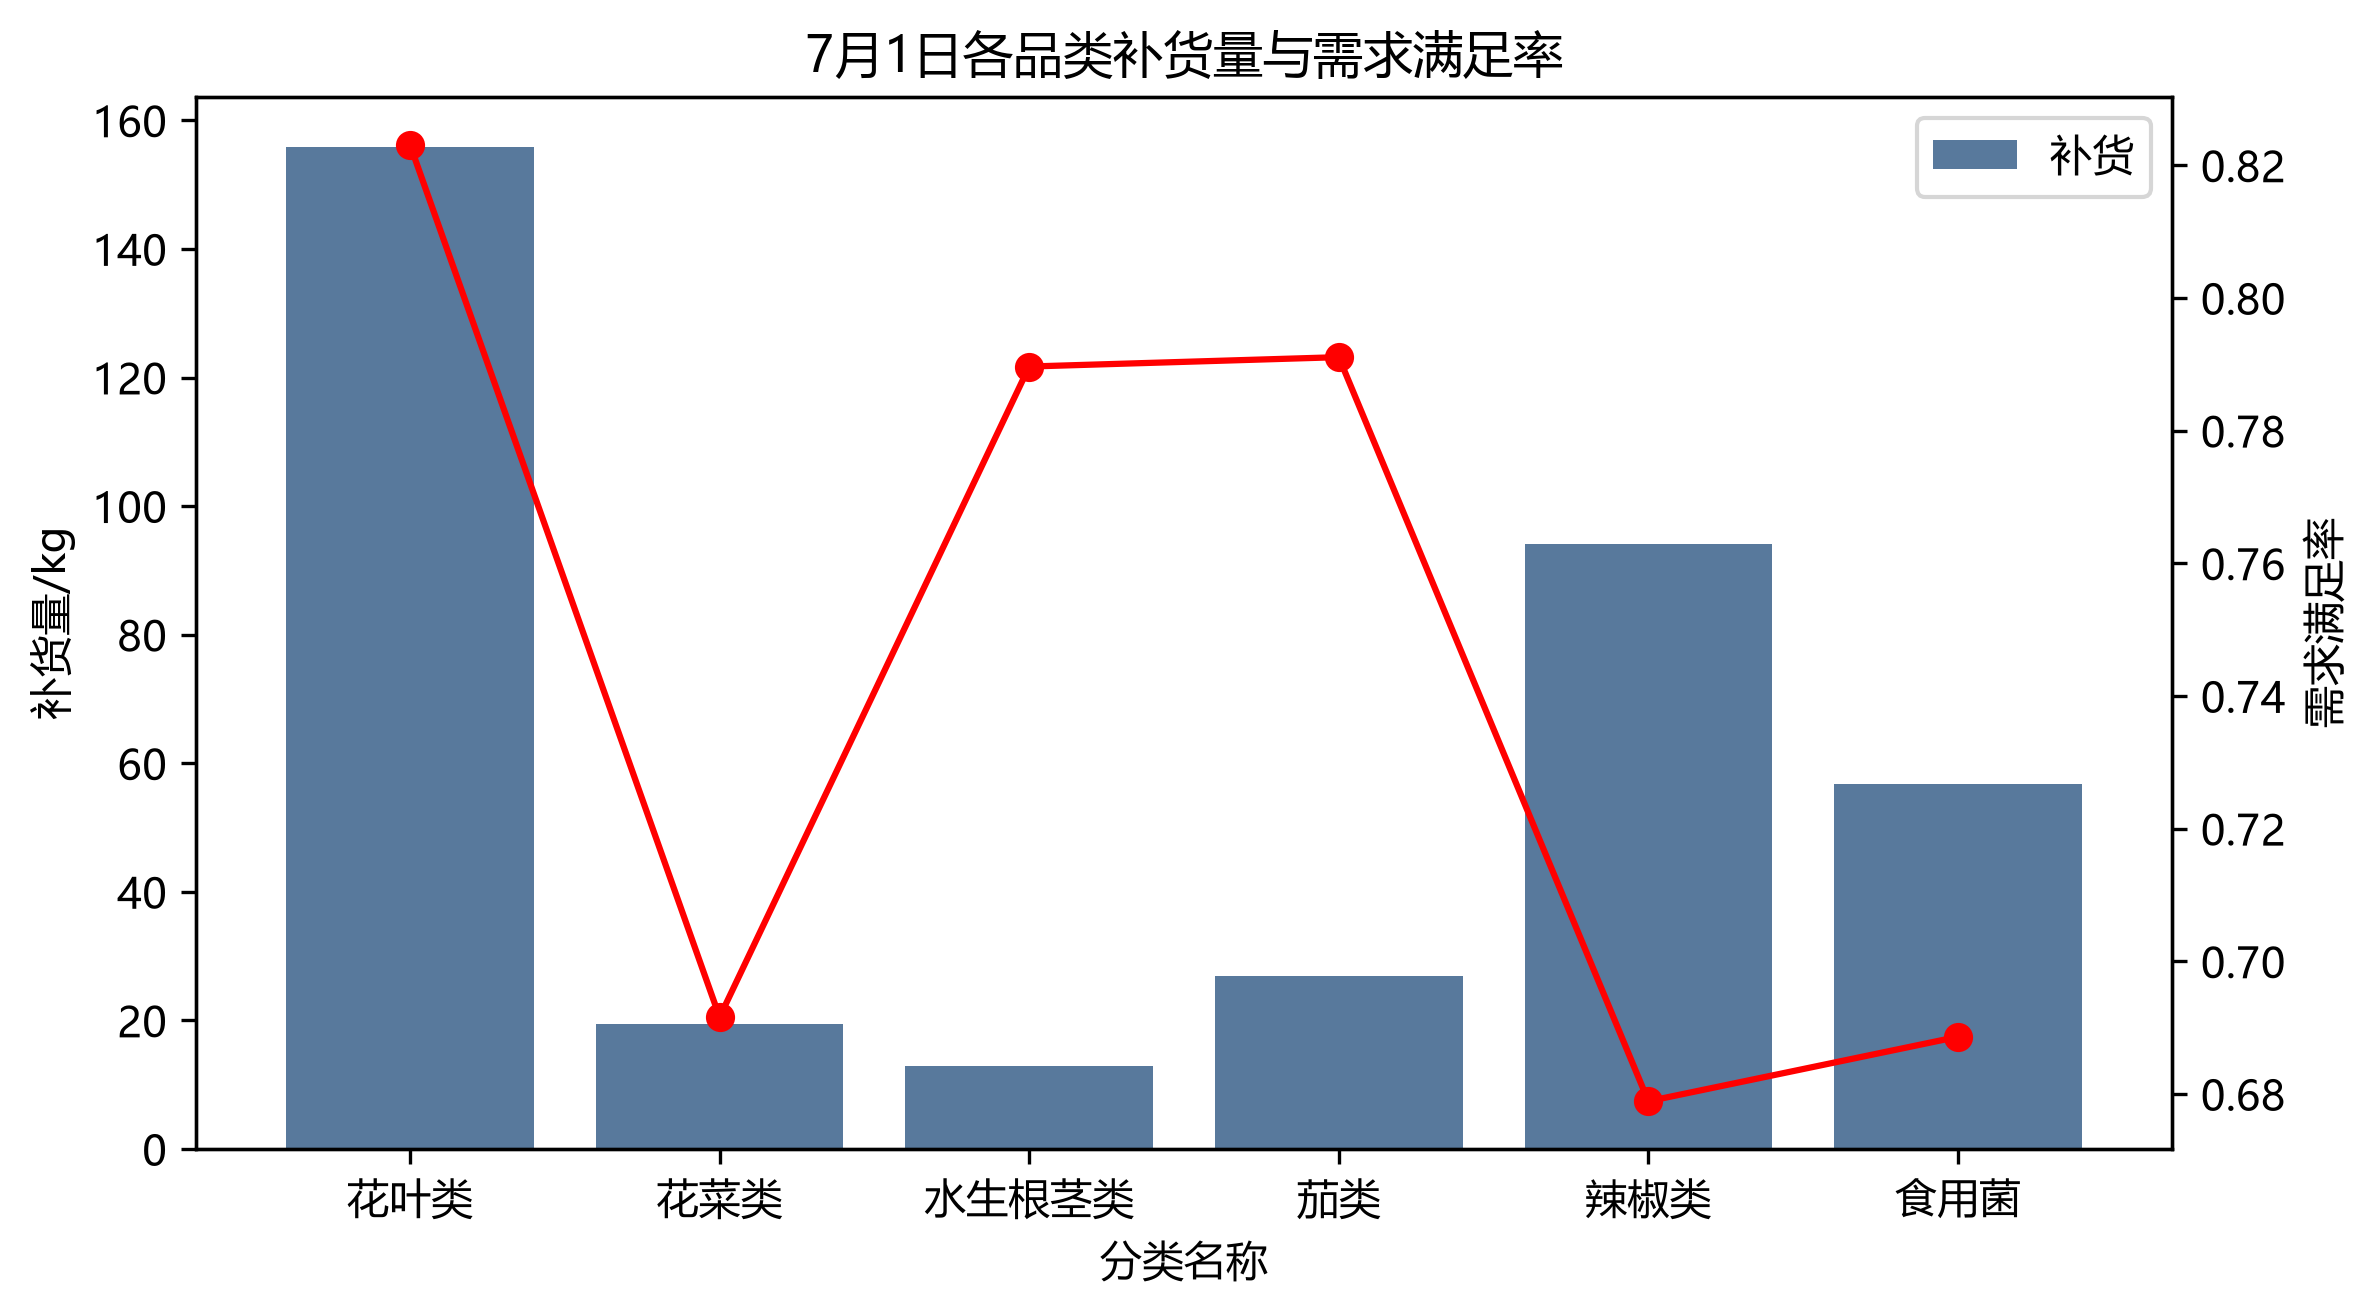
\includegraphics[width=0.85\textwidth]{figures/q3_category_coverage.png}
\caption{补货量与需求满足率}
\label{fig:cov}
\end{figure}

\begin{figure}[H]
\centering
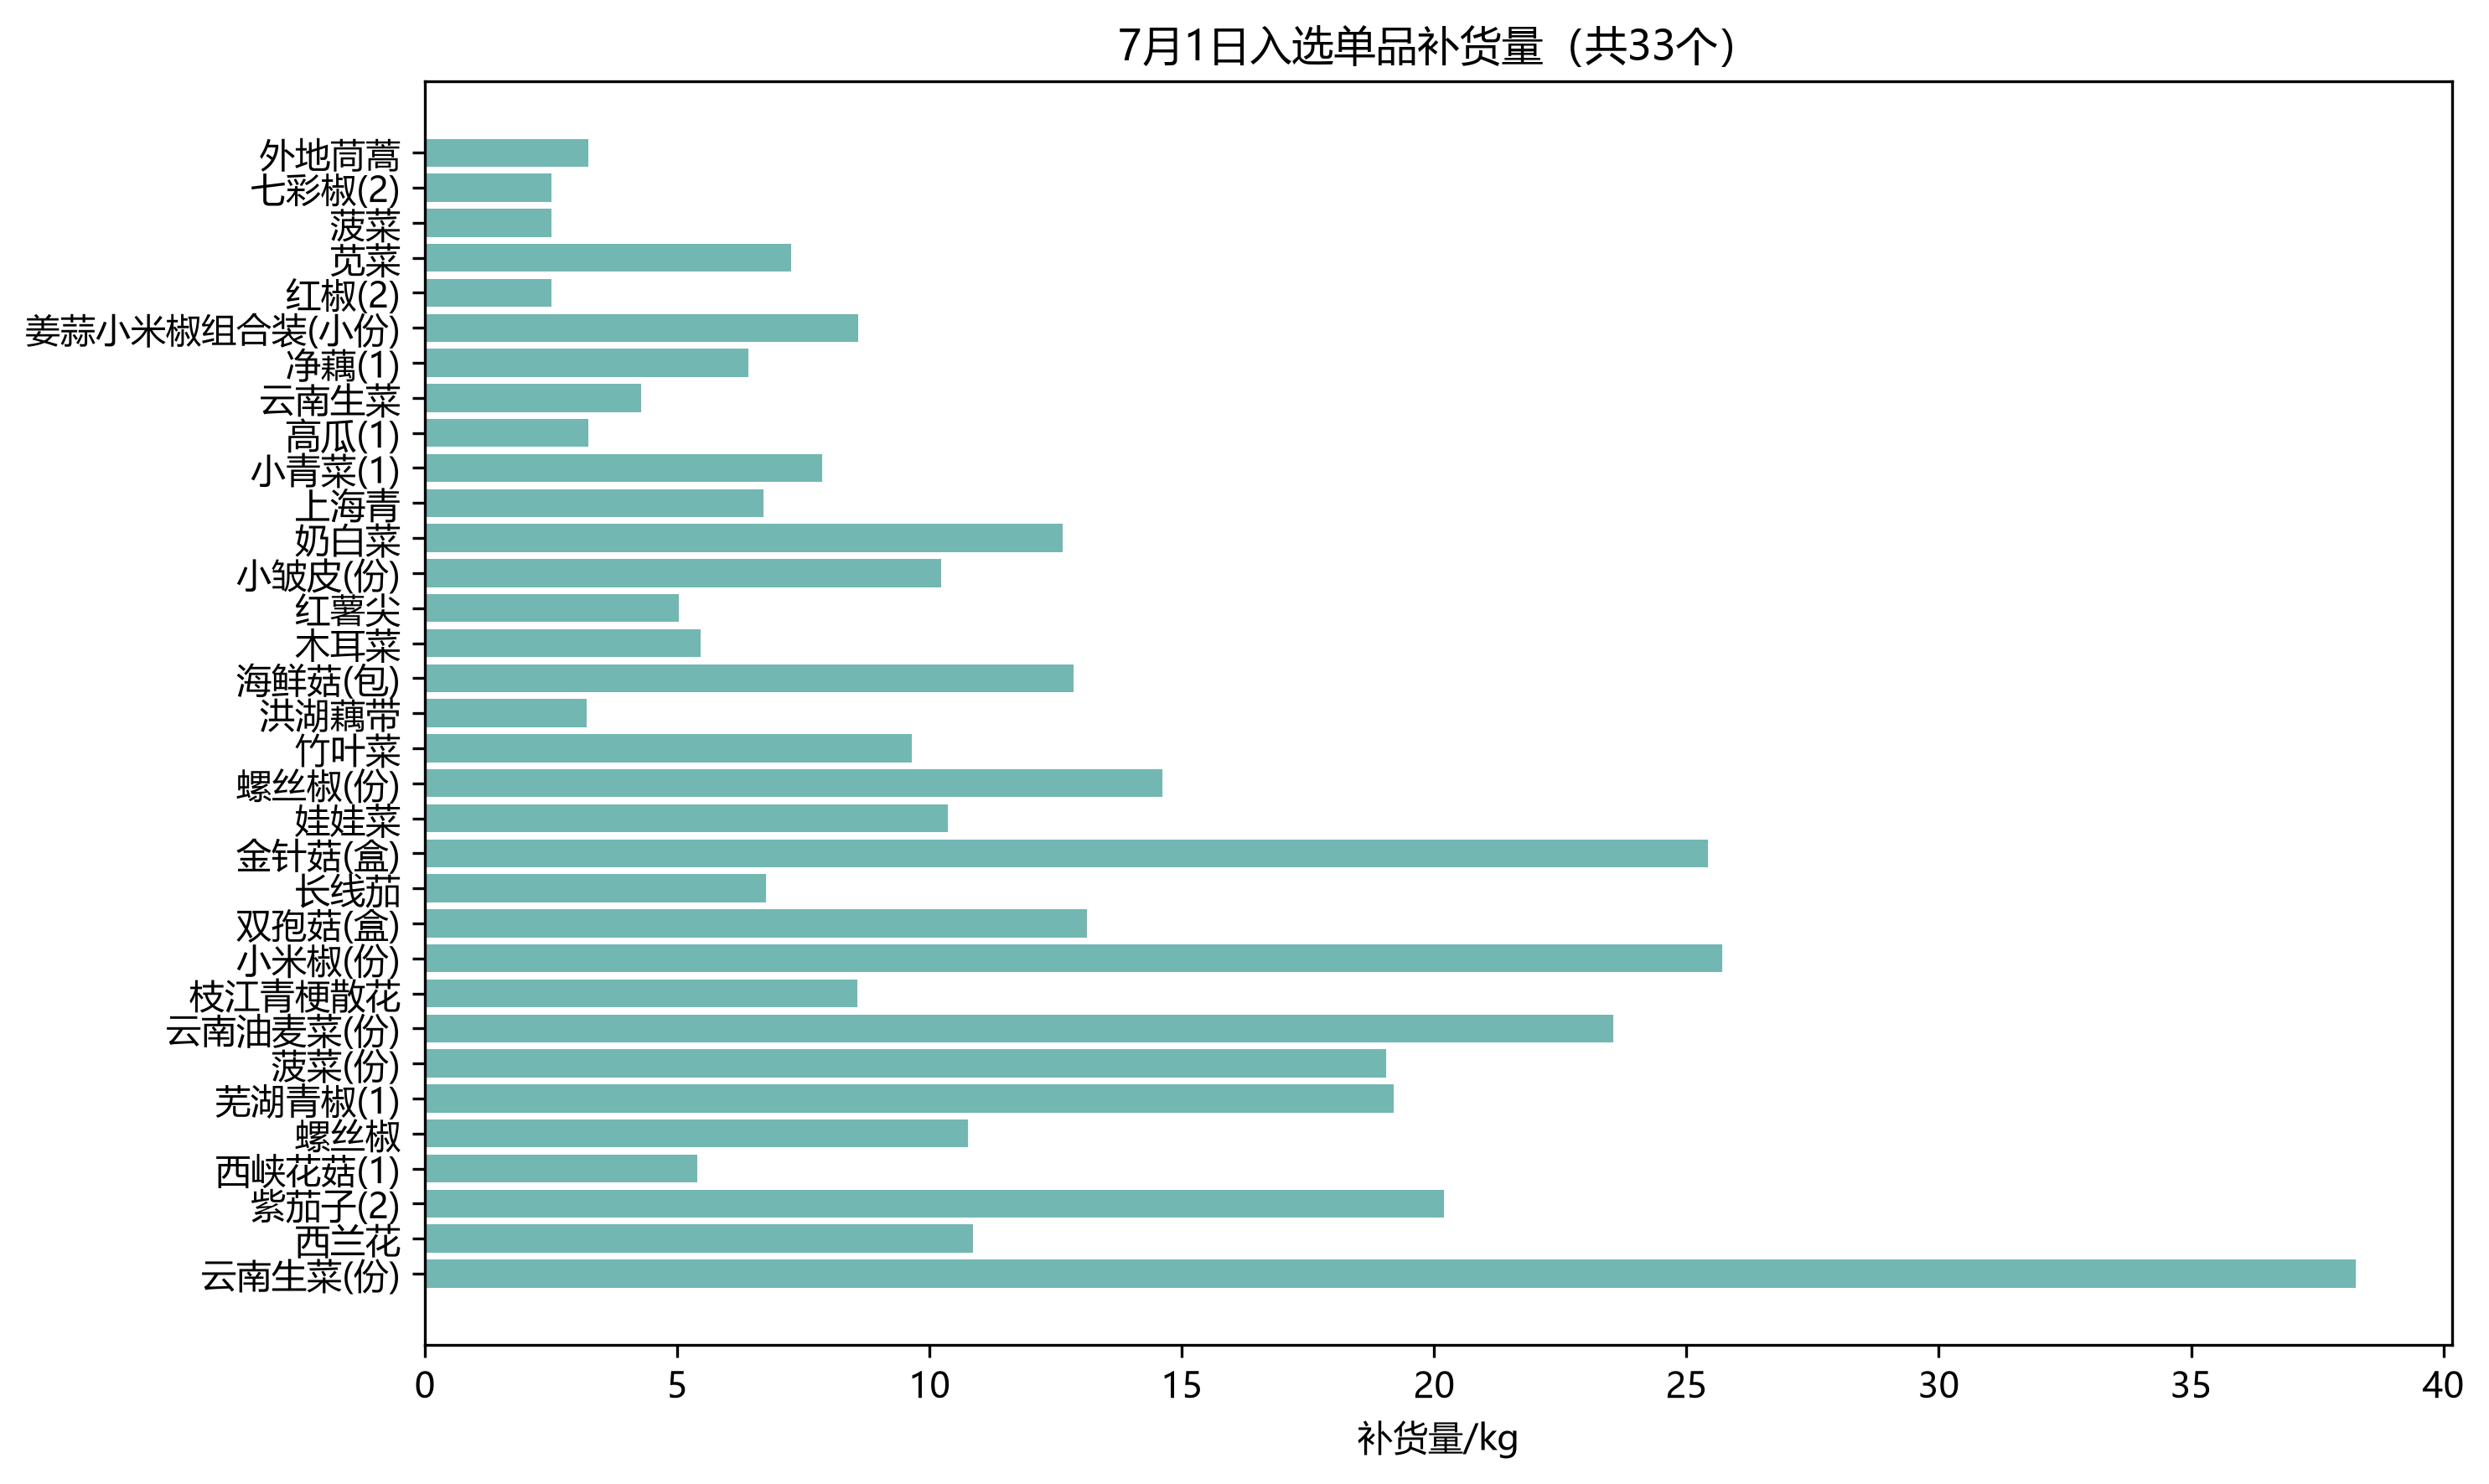
\includegraphics[width=0.95\textwidth]{figures/q3_sku_replenish.png}
\caption{入选单品补货量}
\label{fig:sku}
\end{figure}

\begin{table}[H]
\centering
\caption{7月1日单品补货与定价（入选清单）}
\label{tab:plan3}
\scriptsize
\begin{tabular}{llcccc}
\toprule
单品名称 & 分类名称 & 补货量 & 建议售价 & 加成率 & 单品收益 \\
\hline
洪湖藕带 & 水生根茎类 & 3.20 & 39.60 & 1.20 & 38.69 \\
高瓜(1) & 水生根茎类 & 3.23 & 24.76 & 1.20 & 20.26 \\
净藕(1) & 水生根茎类 & 6.41 & 6.29 & 1.20 & 19.77 \\
云南生菜(份) & 花叶类 & 38.26 & 6.75 & 1.20 & 116.58 \\
菠菜(份) & 花叶类 & 19.05 & 7.00 & 1.20 & 60.13 \\
云南油麦菜(份) & 花叶类 & 23.55 & 5.61 & 1.20 & 59.60 \\
娃娃菜 & 花叶类 & 10.36 & 8.60 & 1.20 & 46.41 \\
竹叶菜 & 花叶类 & 9.65 & 10.16 & 1.20 & 40.16 \\
木耳菜 & 花叶类 & 5.46 & 12.28 & 1.20 & 31.47 \\
红薯尖 & 花叶类 & 5.03 & 12.32 & 1.20 & 28.56 \\
奶白菜 & 花叶类 & 12.63 & 5.52 & 1.20 & 27.11 \\
上海青 & 花叶类 & 6.71 & 8.32 & 1.20 & 22.38 \\
小青菜(1) & 花叶类 & 7.87 & 6.02 & 1.20 & 20.95 \\
云南生菜 & 花叶类 & 4.28 & 11.78 & 1.20 & 19.82 \\
苋菜 & 花叶类 & 7.25 & 7.37 & 1.20 & 19.25 \\
菠菜 & 花叶类 & 2.50 & 21.19 & 1.20 & 17.60 \\
外地茼蒿 & 花叶类 & 3.24 & 17.42 & 1.20 & 16.00 \\
西兰花 & 花菜类 & 10.86 & 20.24 & 1.20 & 99.58 \\
枝江青梗散花 & 花菜类 & 8.56 & 15.20 & 1.20 & 58.71 \\
紫茄子(2) & 茄类 & 20.19 & 9.00 & 1.20 & 88.07 \\
长线茄 & 茄类 & 6.76 & 16.63 & 1.20 & 53.55 \\
螺丝椒 & 辣椒类 & 10.76 & 14.56 & 1.20 & 69.50 \\
芜湖青椒(1) & 辣椒类 & 19.20 & 7.35 & 1.20 & 68.91 \\
小米椒(份) & 辣椒类 & 25.70 & 4.99 & 1.20 & 57.91 \\
螺丝椒(份) & 辣椒类 & 14.61 & 6.77 & 1.20 & 44.60 \\
小皱皮(份) & 辣椒类 & 10.24 & 5.87 & 1.20 & 27.13 \\
姜蒜小米椒组合装(小份) & 辣椒类 & 8.59 & 5.04 & 1.20 & 19.52 \\
红椒(2) & 辣椒类 & 2.50 & 28.16 & 1.20 & 19.29 \\
七彩椒(2) & 辣椒类 & 2.50 & 21.38 & 1.20 & 17.15 \\
西峡花菇(1) & 食用菌 & 5.39 & 33.44 & 1.20 & 78.83 \\
双孢菇(盒) & 食用菌 & 13.12 & 7.63 & 1.20 & 54.43 \\
金针菇(盒) & 食用菌 & 25.42 & 3.78 & 1.20 & 52.03 \\
海鲜菇(包) & 食用菌 & 12.86 & 4.62 & 1.20 & 32.40 \\
\bottomrule
\end{tabular}
\end{table}

\begin{figure}[H]
\centering
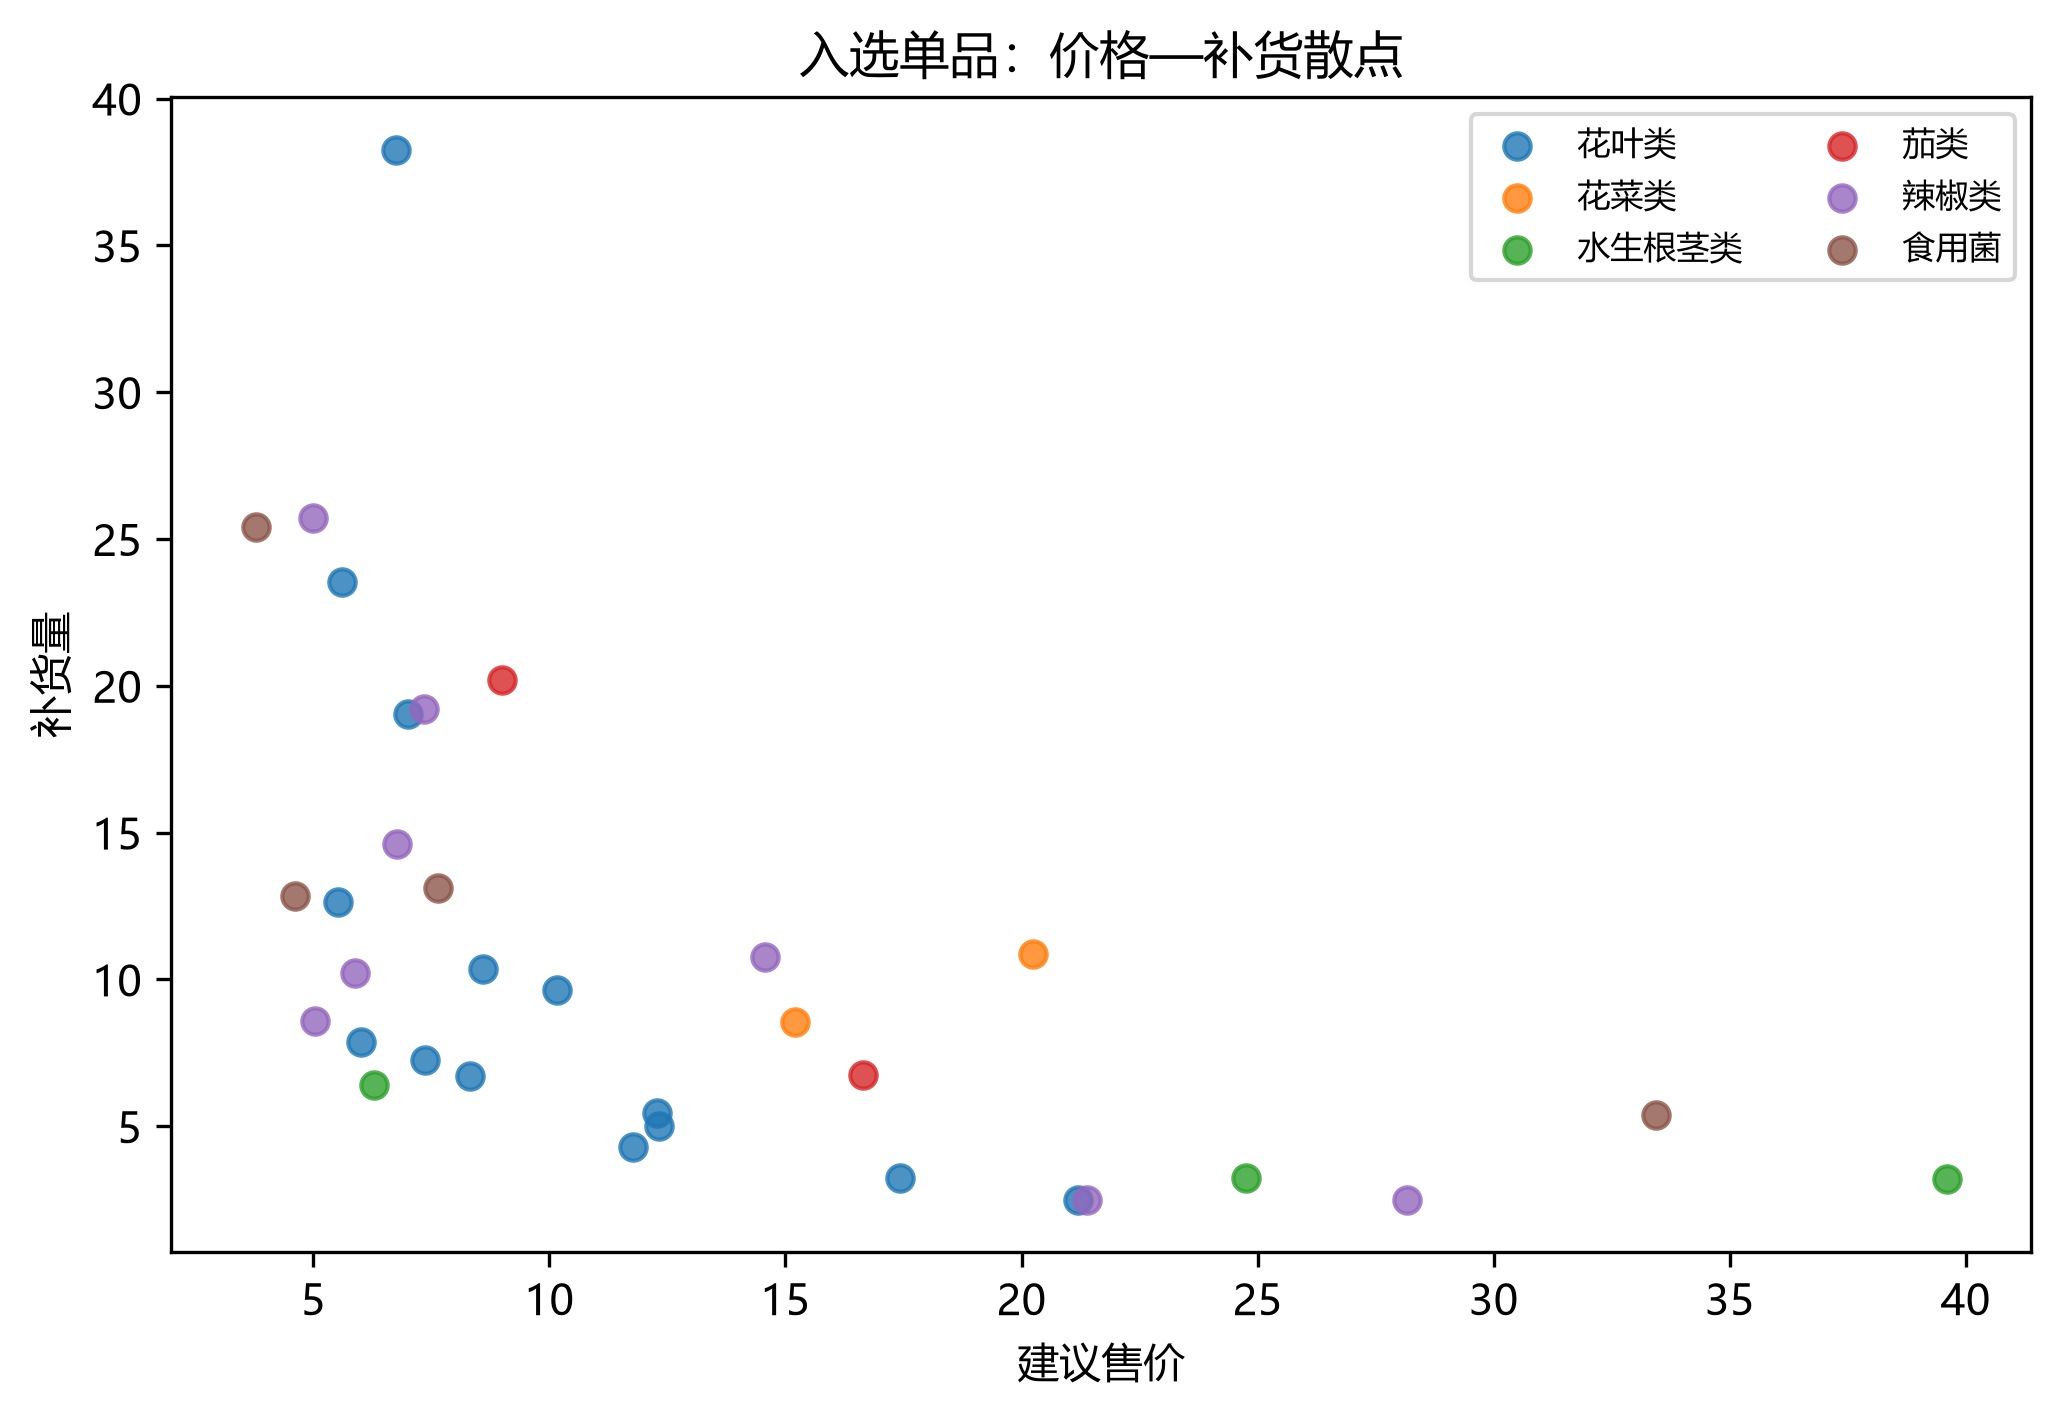
\includegraphics[width=0.85\textwidth]{figures/q3_price_qty_selected.png}
\caption{入选单品价格—补货散点}
\label{fig:pq}
\end{figure}

\section{问题4：数据采集建议}
结合残差诊断、星期变异与打折效应（图~\ref{fig:q4a}--\ref{fig:q4b}），按``对误差贡献最大优先''提出补采清单：
\begin{enumerate}[leftmargin=2em]
\item \textbf{实时库存/日终剩余}：把销量与需求解耦，纠正缺货截断，直接改善Q2/Q3补货量；
\item \textbf{客流与转化}：解释星期与峰时波动，降低把价格当作唯一需求驱动的偏误；
\item \textbf{天气与节假日}：蔬菜需求对高温降雨敏感，可提升短期预测稳定性；
\item \textbf{促销档期与陈列位置}：解释打折强度与空间约束，服务27--33单品组合；
\item \textbf{供应商准时率与品质}：降低只按历史销量选品的供应风险。
\end{enumerate}

\begin{figure}[H]
\centering
\begin{minipage}{0.48\textwidth}
\centering
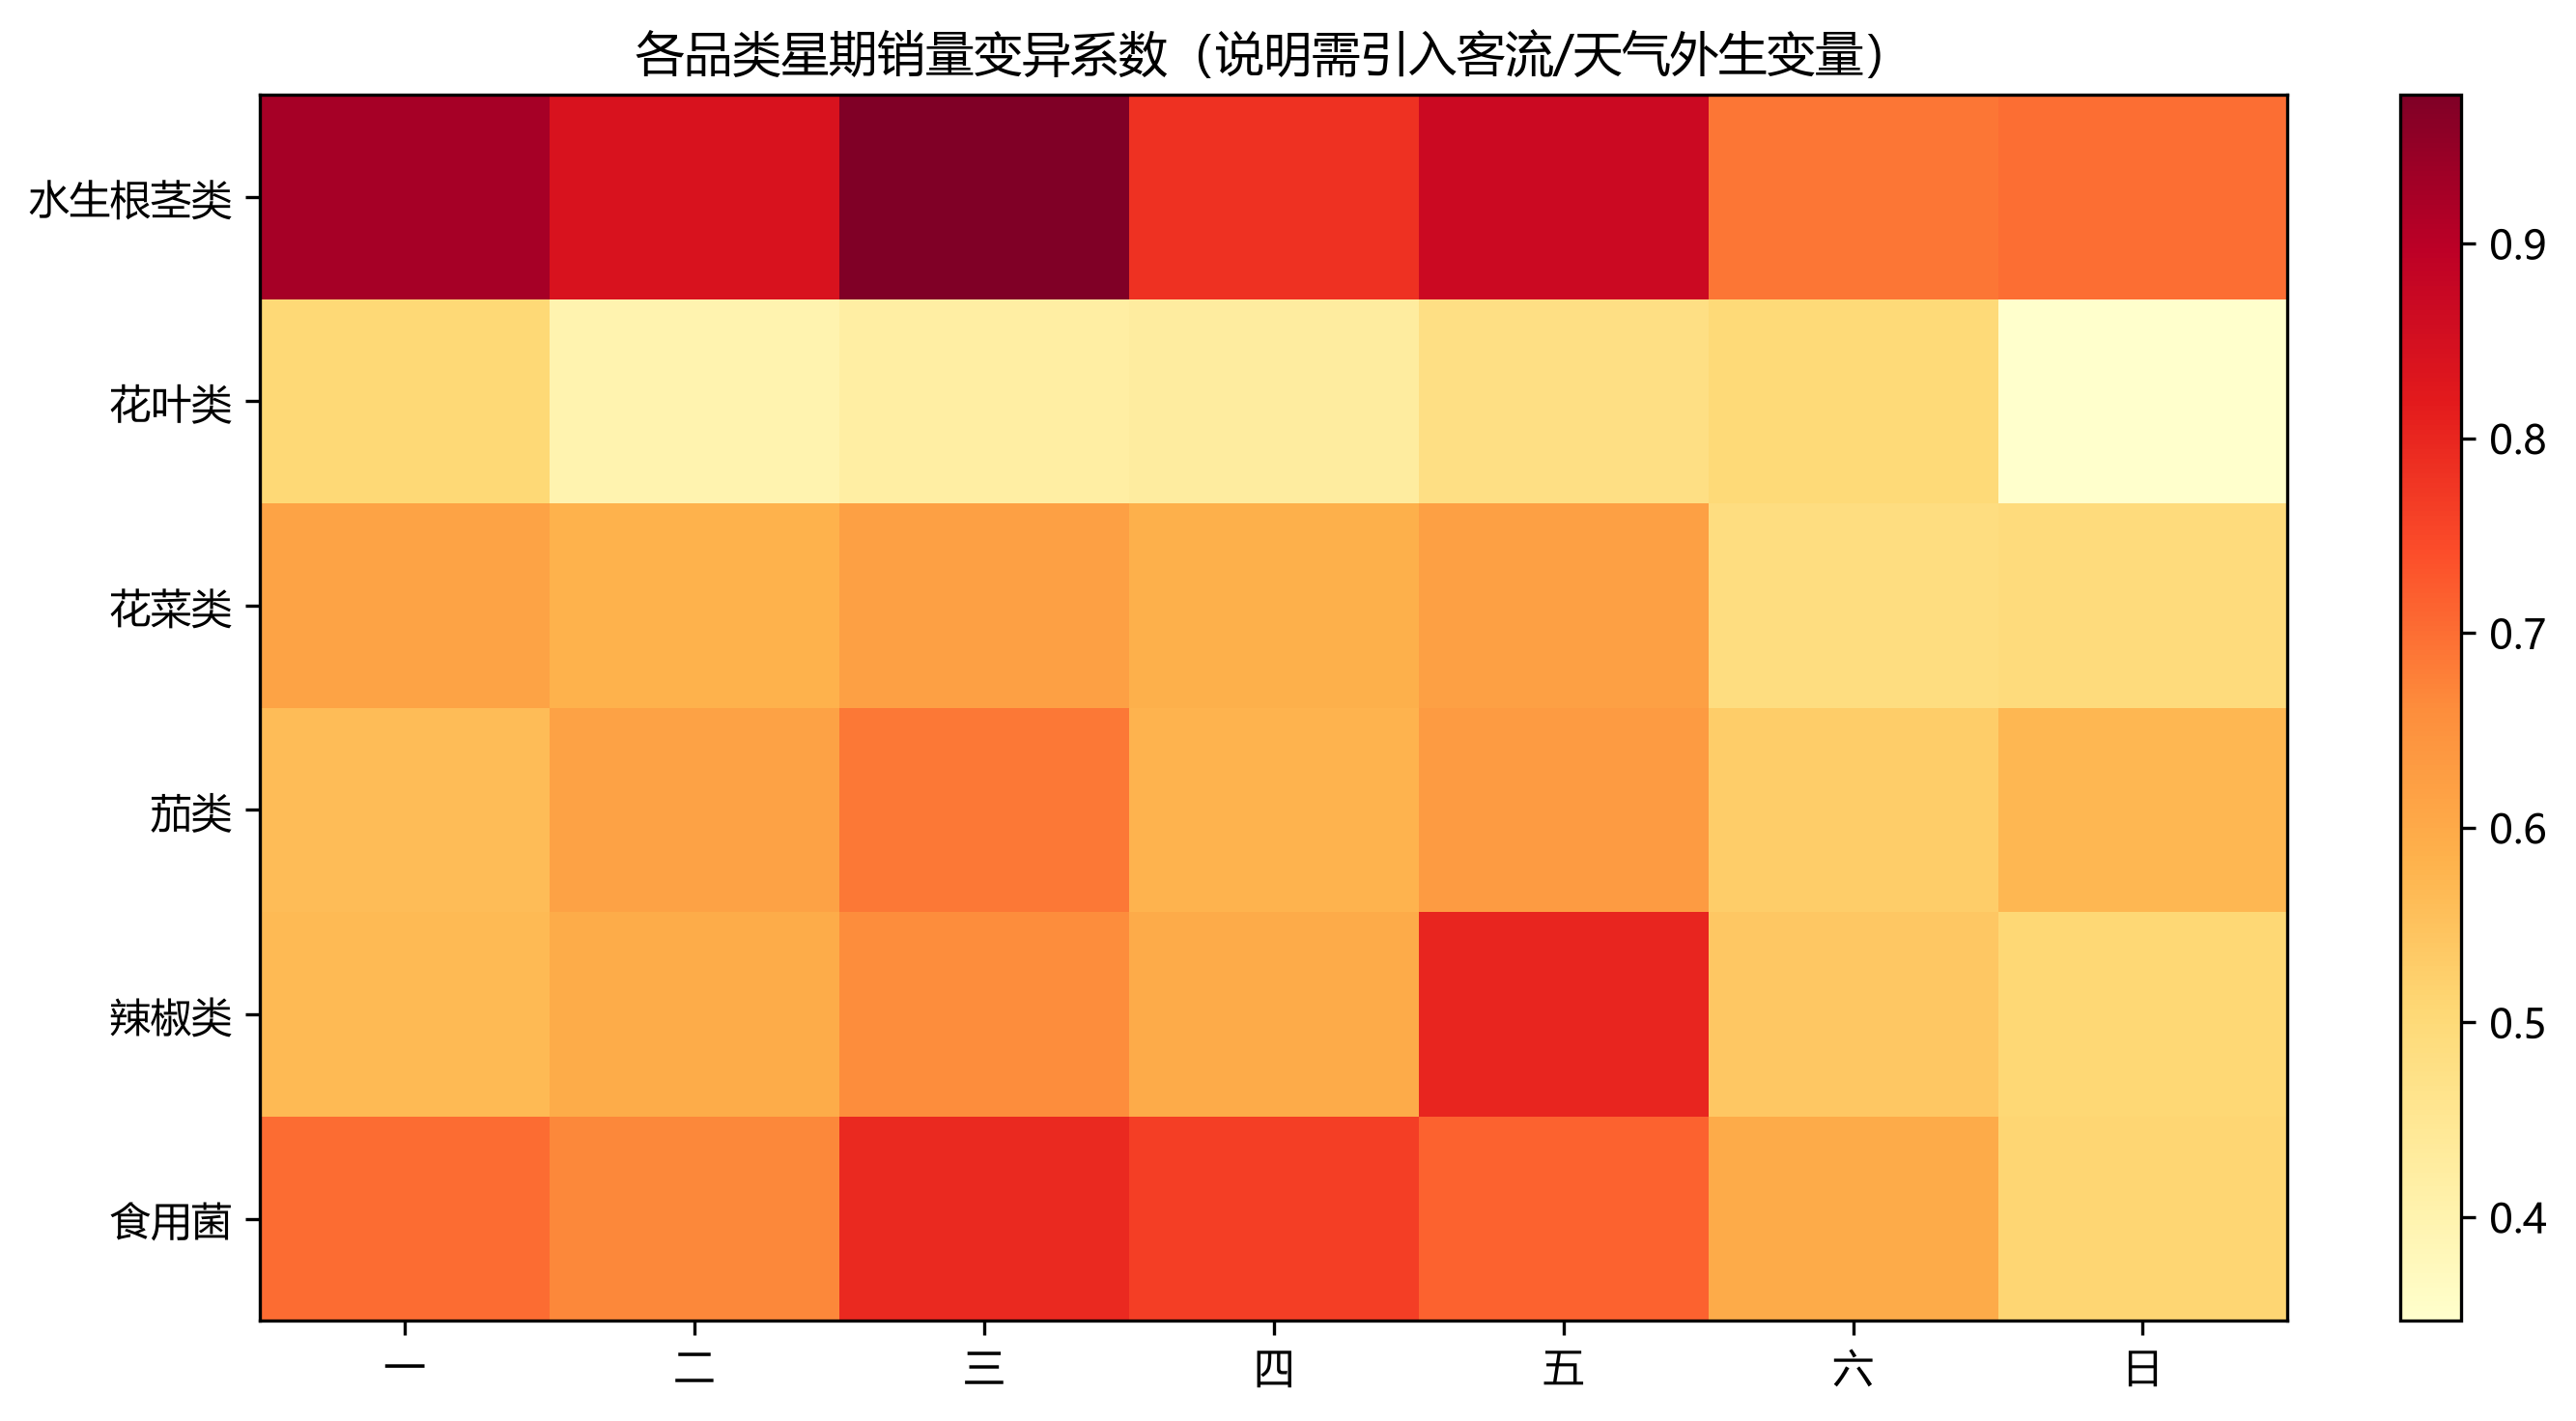
\includegraphics[width=\linewidth]{figures/q4_weekday_cv_heatmap.png}
\caption{星期销量变异系数}
\label{fig:q4a}
\end{minipage}
\hfill
\begin{minipage}{0.48\textwidth}
\centering
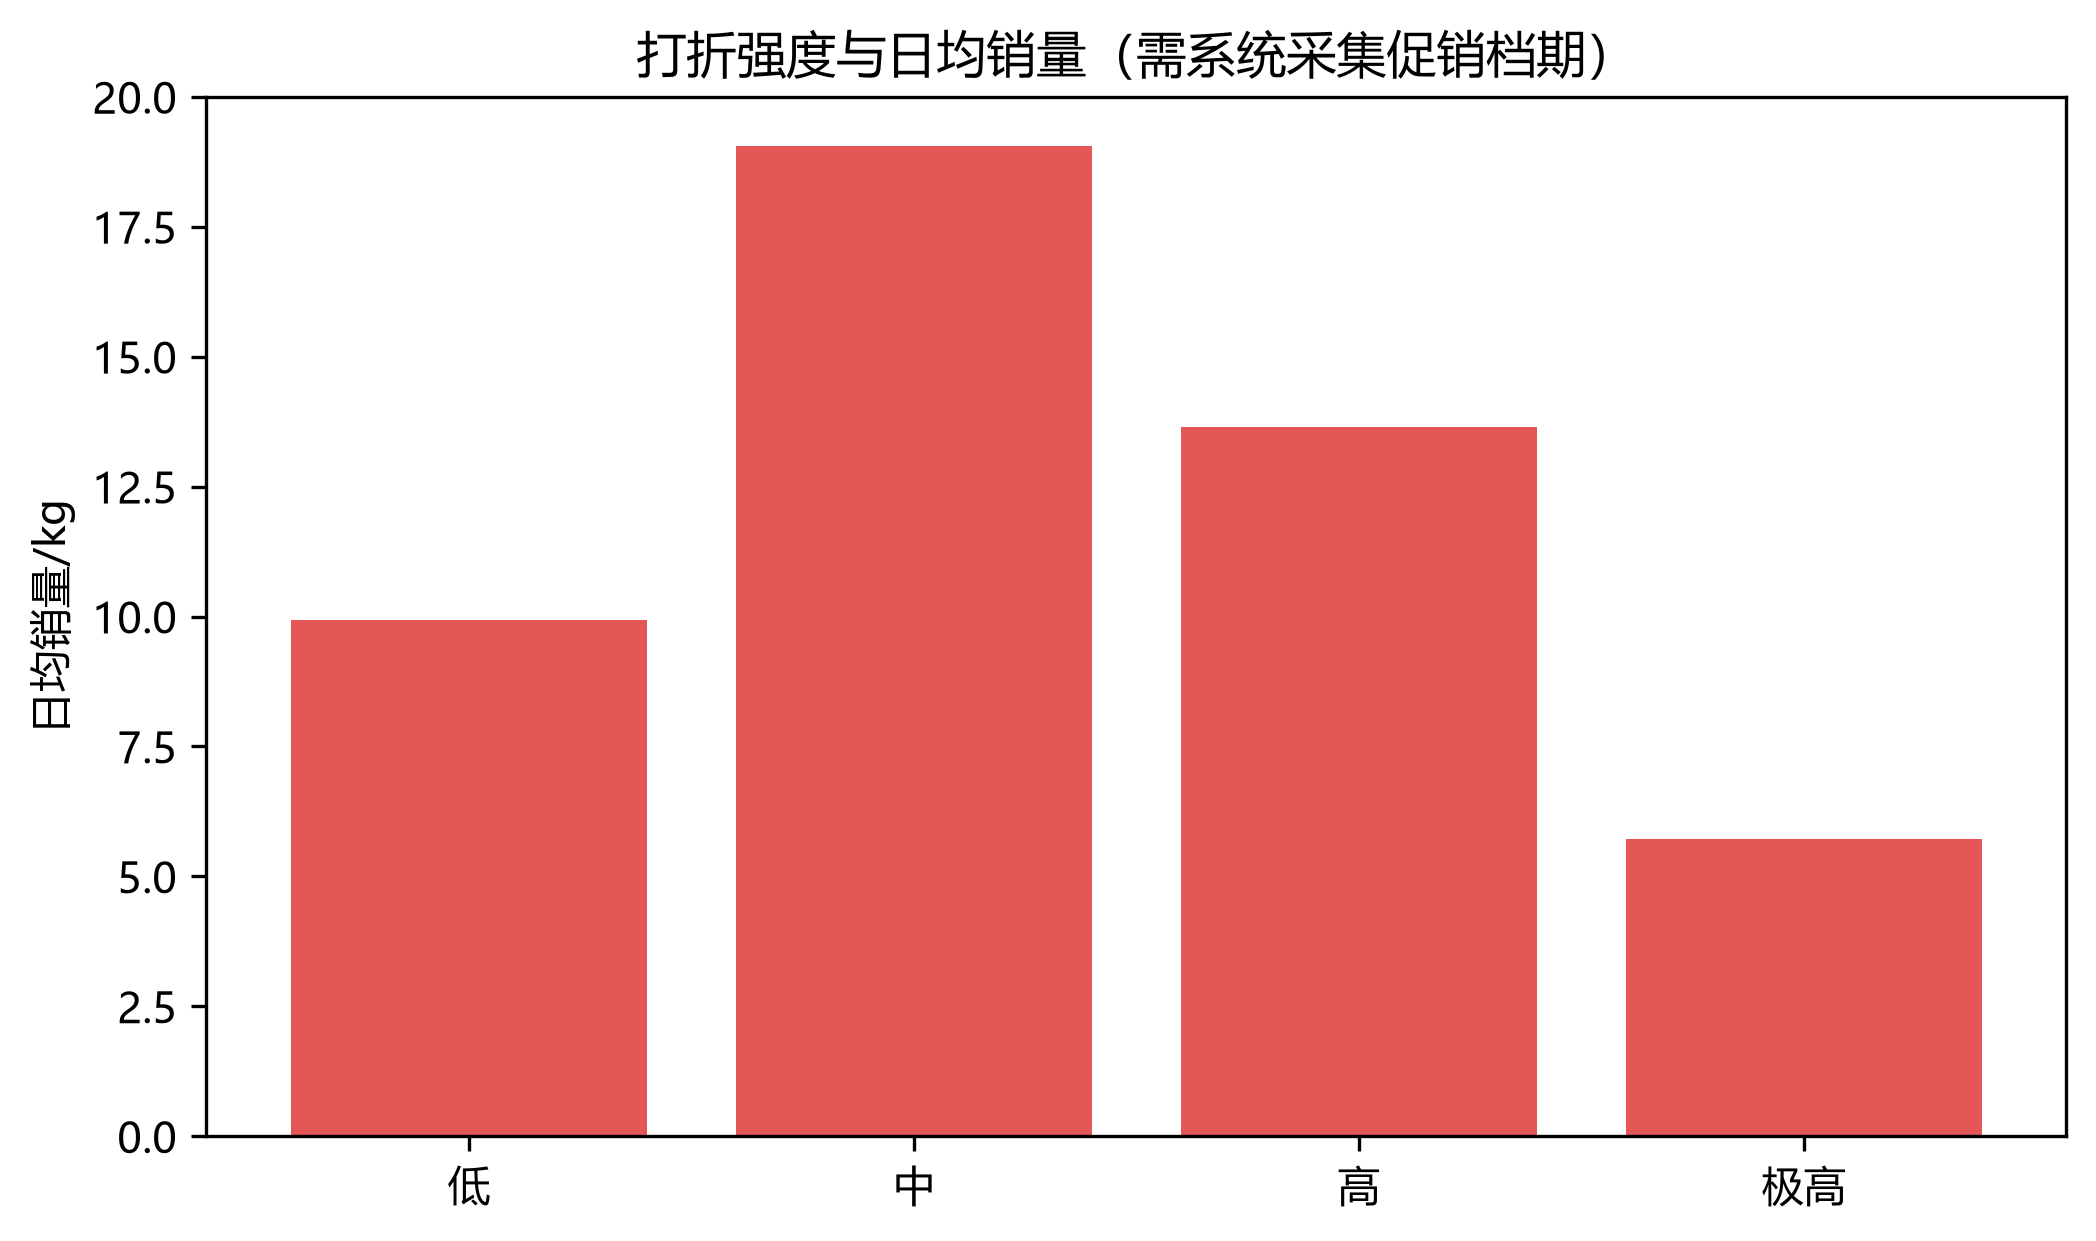
\includegraphics[width=\linewidth]{figures/q4_discount_impact.png}
\caption{打折强度与销量}
\label{fig:q4b}
\end{minipage}
\end{figure}

\section{模型检验}
\subsection{有效性对比与消融}
消融结果见图~\ref{fig:ablation}：Q2主模型优于历史加成与固定30\%；Q3的ILP优于贪心收益/销量与随机选品。

\begin{figure}[H]
\centering
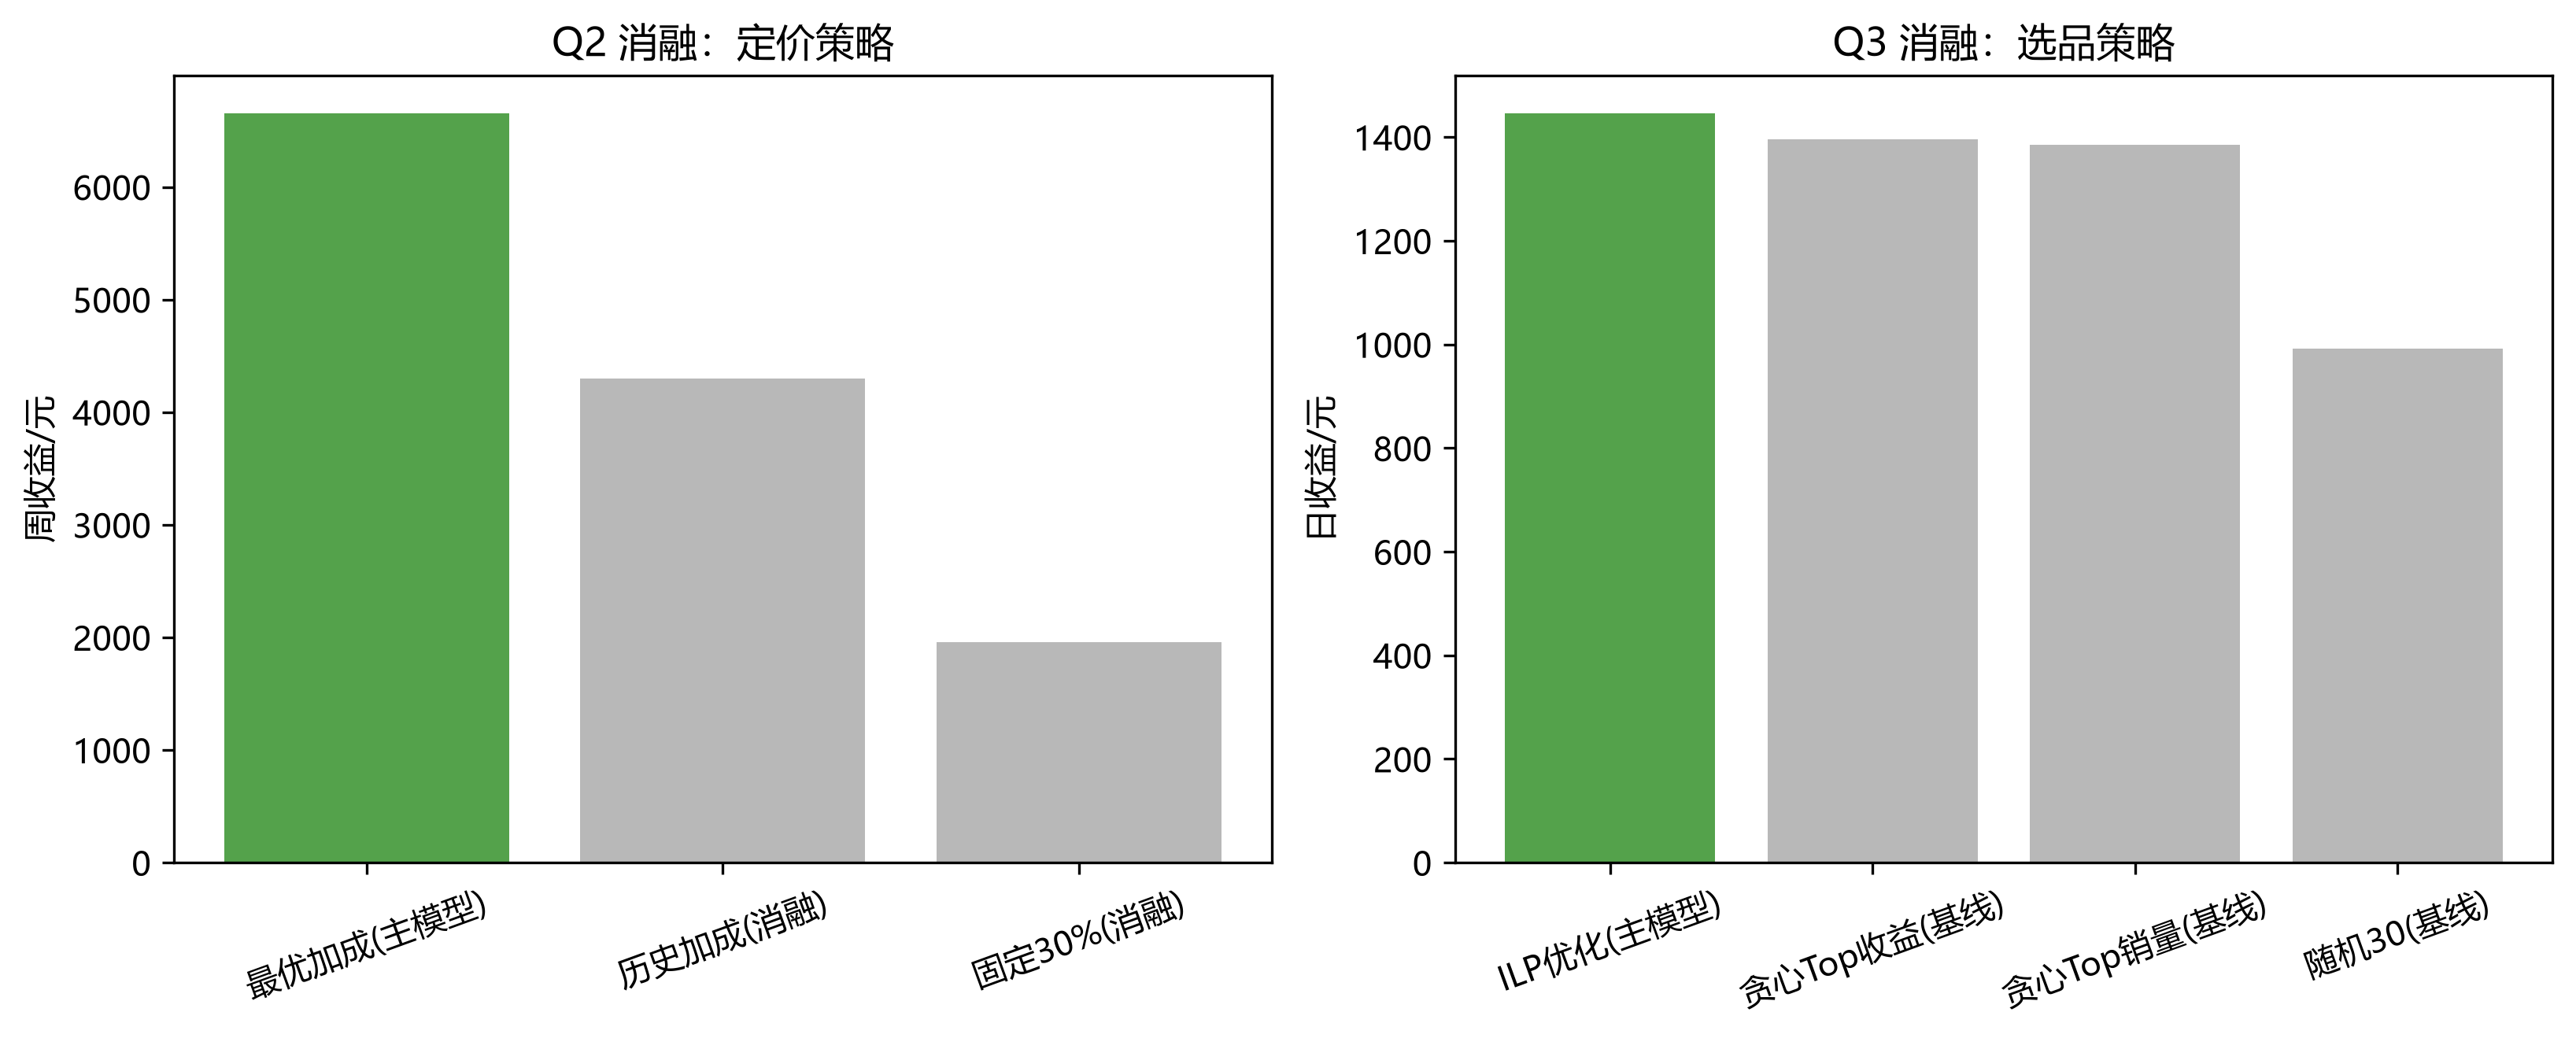
\includegraphics[width=0.95\textwidth]{figures/ablation_compare.png}
\caption{消融与方法对比}
\label{fig:ablation}
\end{figure}

\subsection{灵敏度分析}
对损耗率缩放、加成率偏离与弹性缩放的周收益响应见图~\ref{fig:sens}。可见最优加成附近较平坦，但损耗被低估时收益高估风险显著，提示损耗数据质量关键。

\begin{figure}[H]
\centering
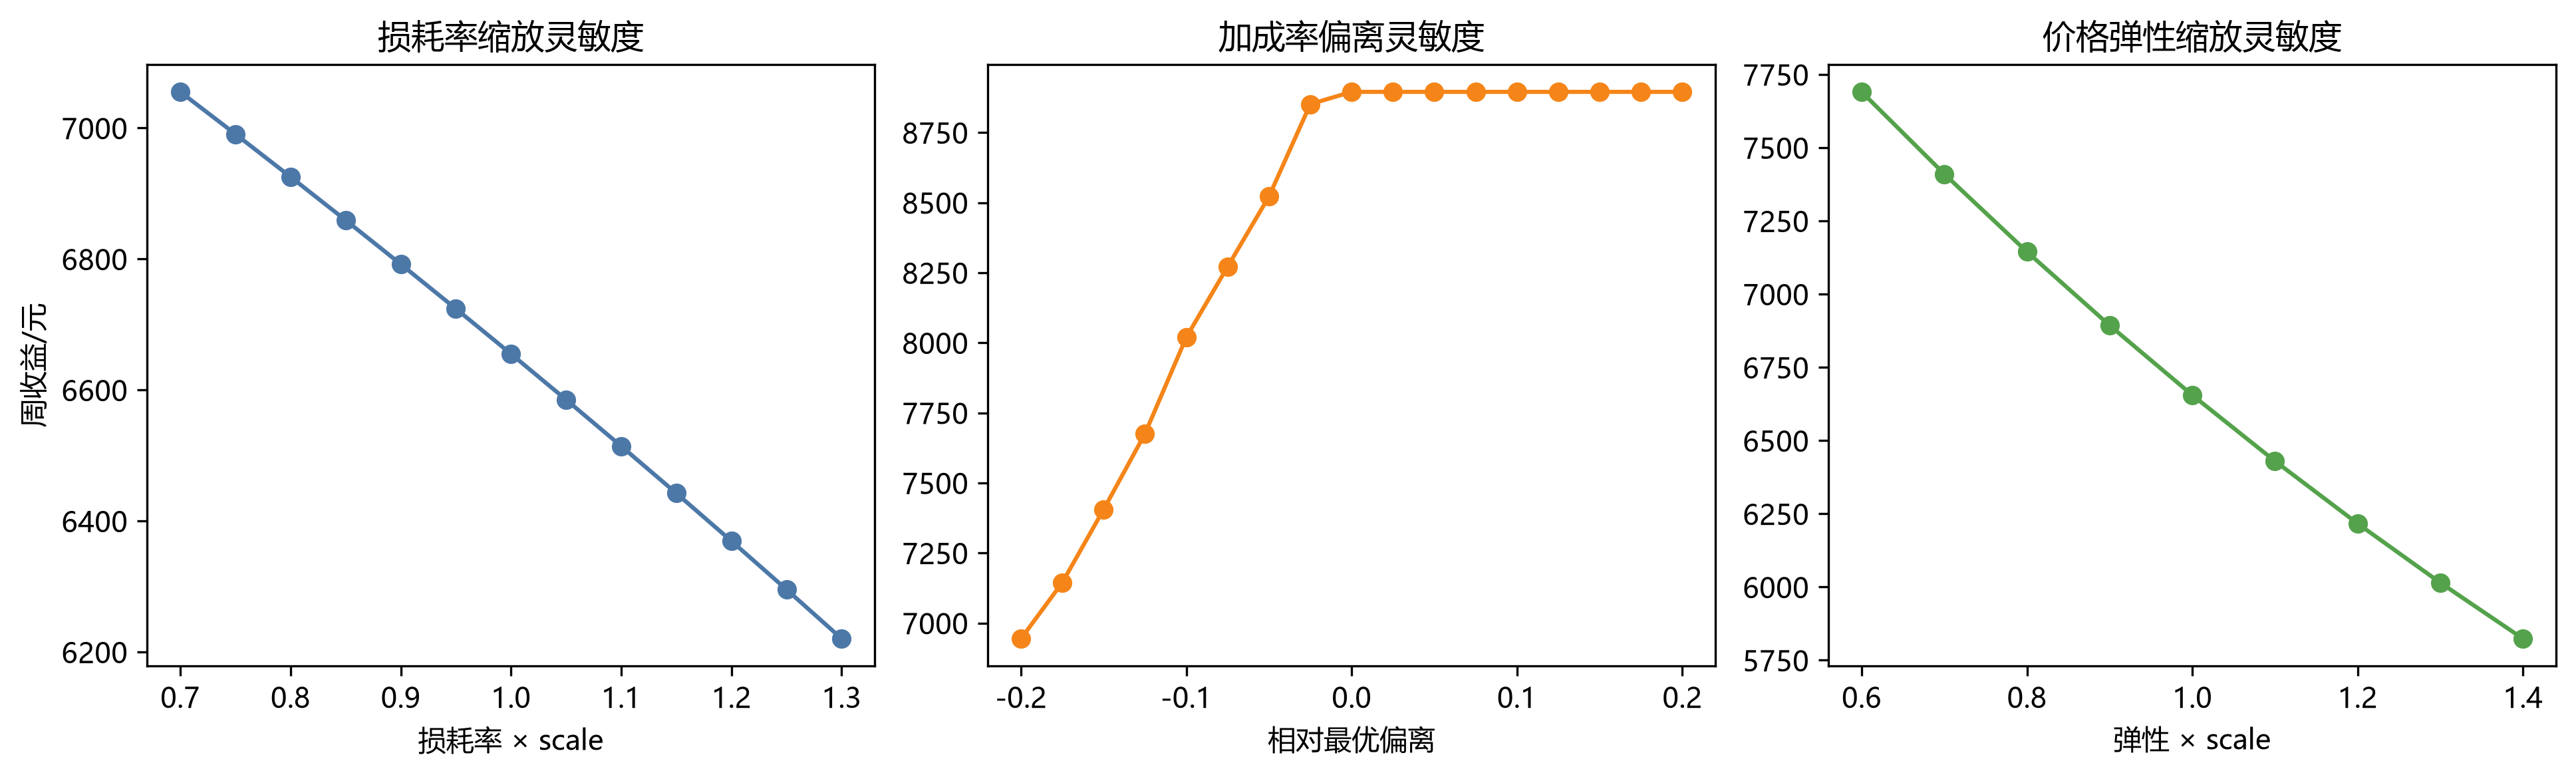
\includegraphics[width=0.98\textwidth]{figures/sens_q2_three_params.png}
\caption{关键参数灵敏度}
\label{fig:sens}
\end{figure}

\subsection{鲁棒性检验}
对需求与成本施加对数正态扰动（$n=200$），周收益分布见图~\ref{fig:mc}。均值\textbf{6664.79}元，5\%--95\%分位[\textbf{6295.39},\textbf{7055.26}]，不低于基线95\%水平的概率为\textbf{93.00\%}。单品层噪声重选分布见图~\ref{fig:mc3}。

\begin{figure}[H]
\centering
\begin{minipage}{0.48\textwidth}
\centering
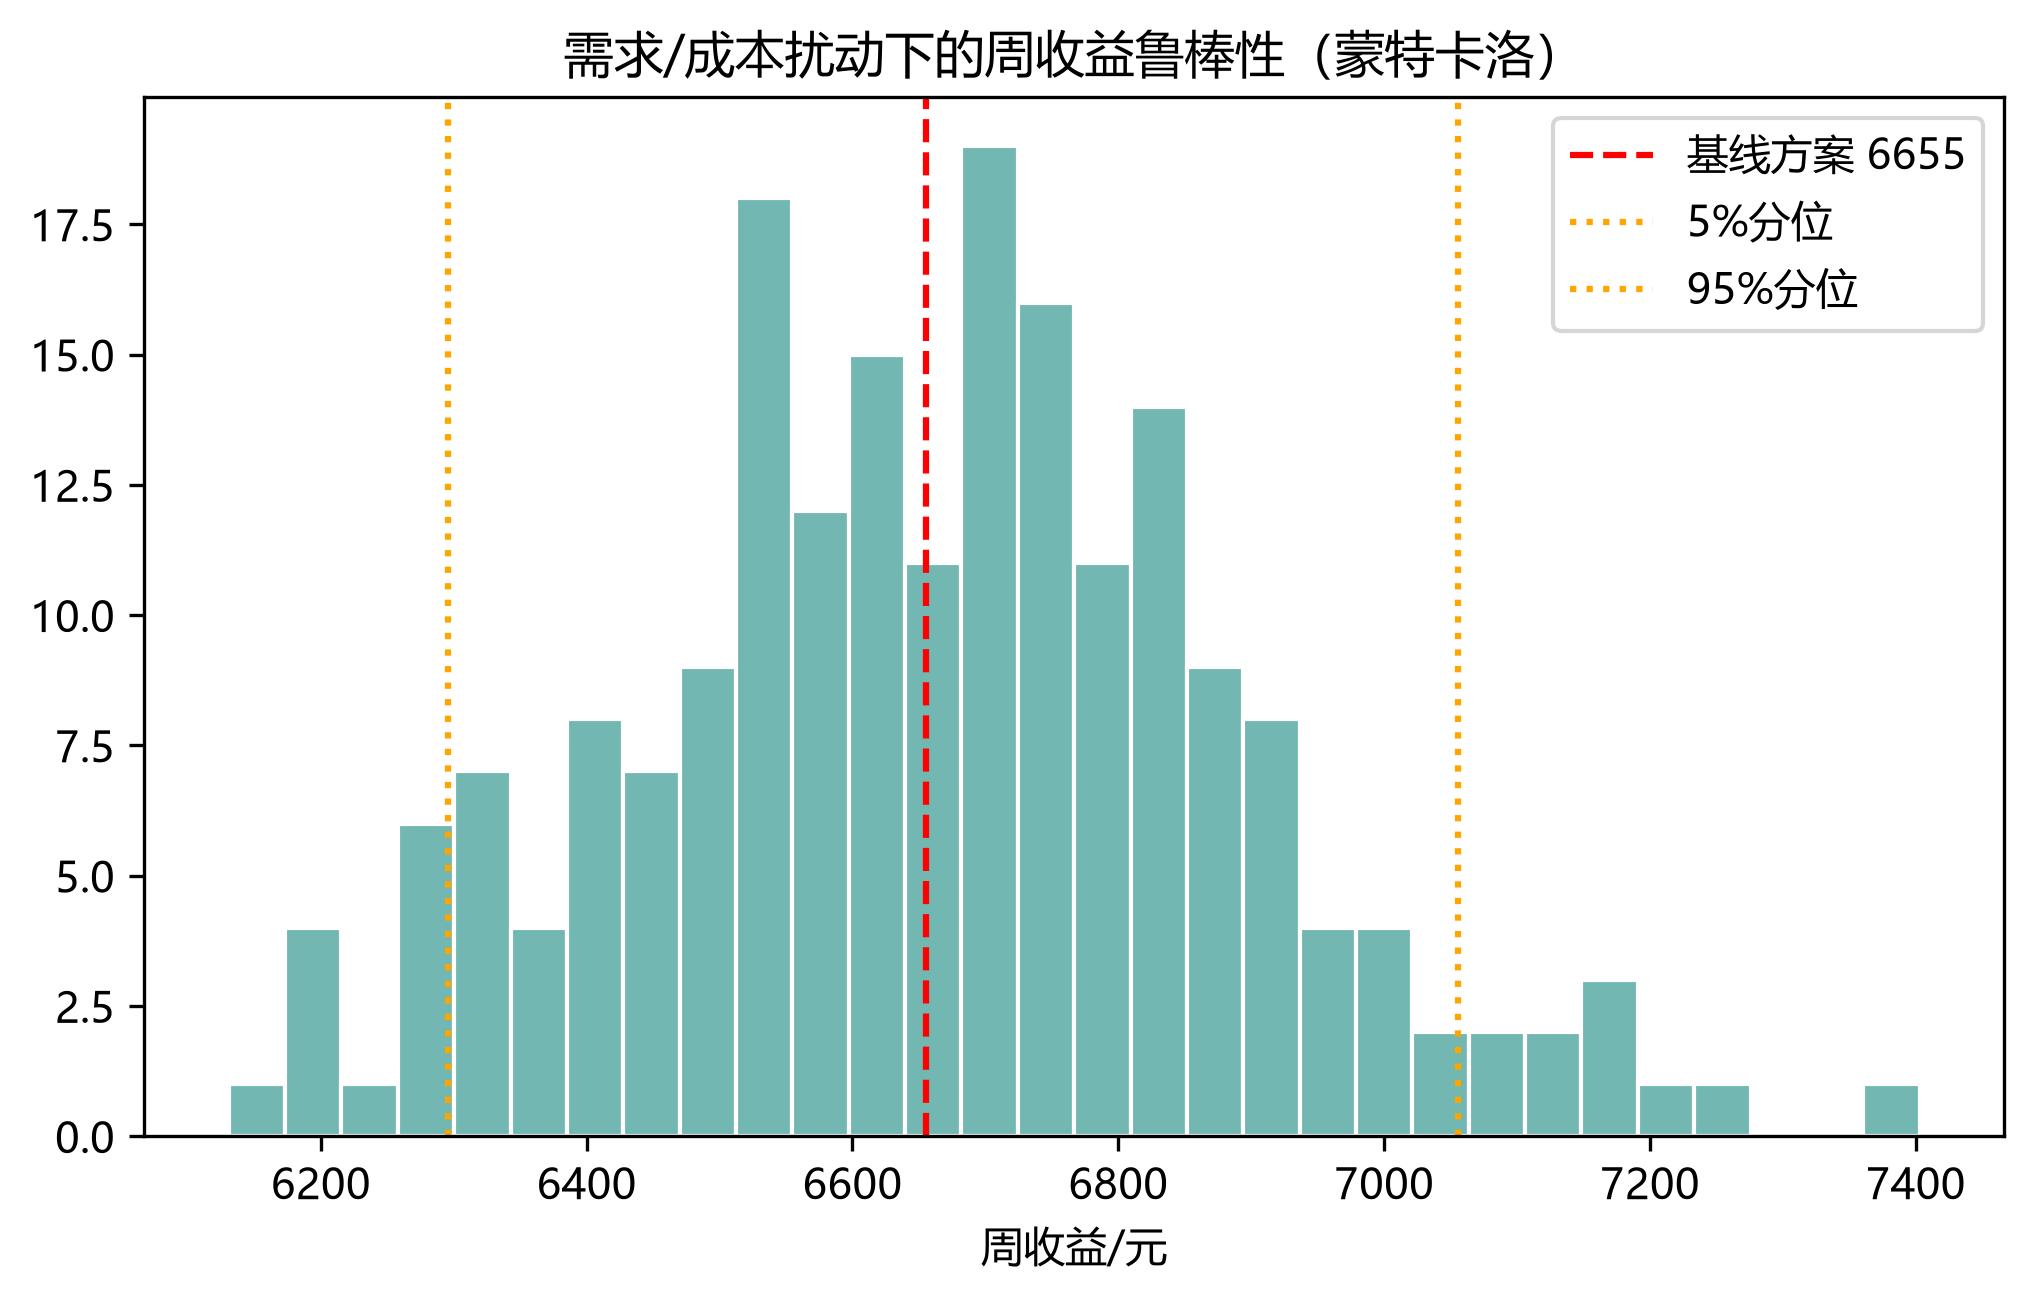
\includegraphics[width=\linewidth]{figures/robust_mc_profit_hist.png}
\caption{Q2蒙特卡洛收益分布}
\label{fig:mc}
\end{minipage}
\hfill
\begin{minipage}{0.48\textwidth}
\centering
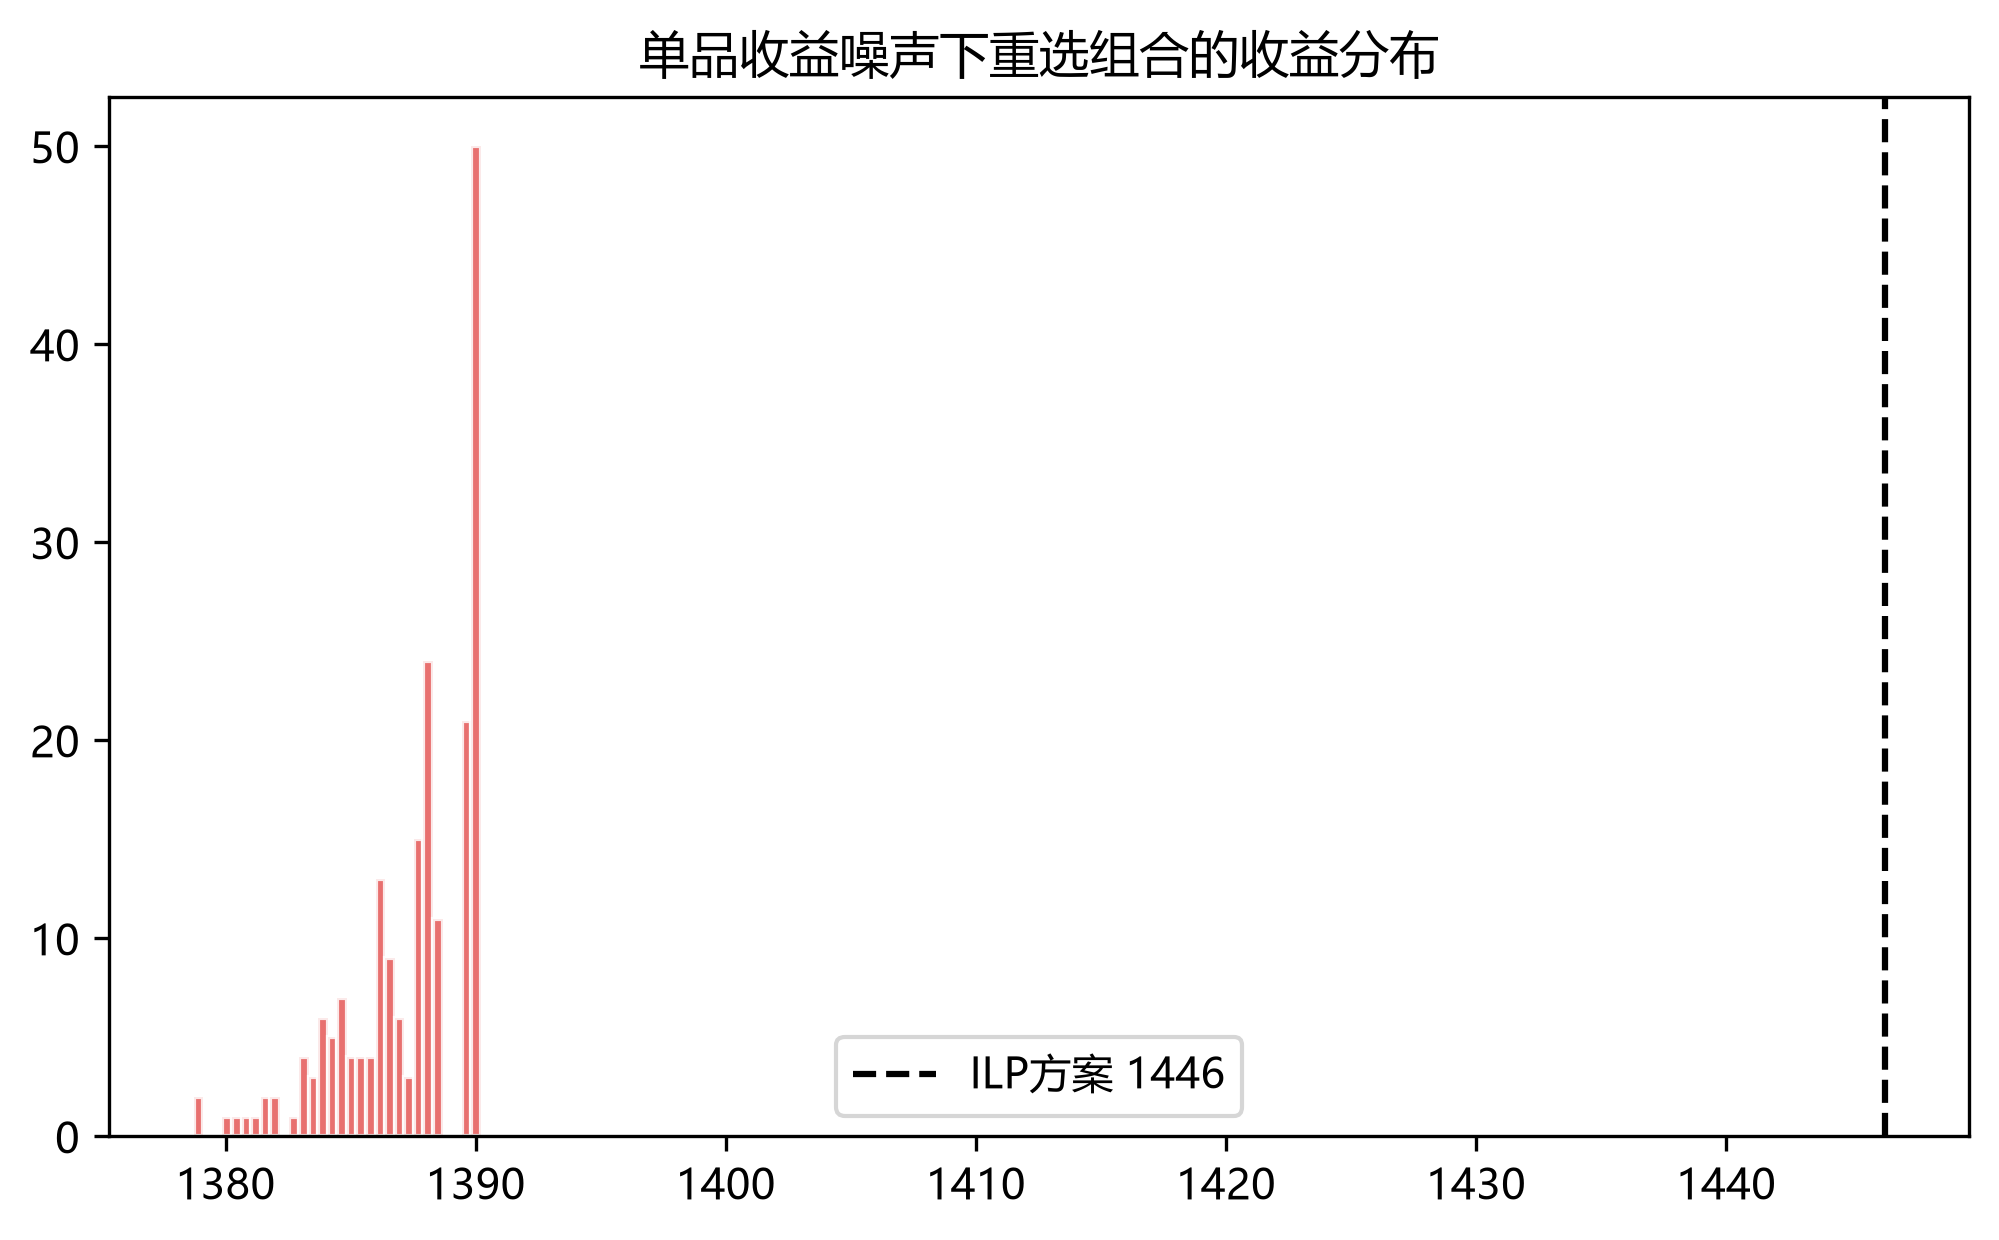
\includegraphics[width=\linewidth]{figures/robust_q3_reselect_hist.png}
\caption{Q3噪声重选收益分布}
\label{fig:mc3}
\end{minipage}
\end{figure}

\subsection{误差与局限}
\begin{enumerate}[leftmargin=2em]
\item 缺真实库存时，销量可能低估潜在需求（右侧截断）；
\item 小票重构存在并发误差，关联规则偏探索性；
\item 批发价预测采用近期中位数，未显式建模供应冲击；
\item Q3品类需求为软约束，极端情况下部分品类满足率可能偏低。
\end{enumerate}

\section{模型评价与推广}
\subsection{优点}
\begin{enumerate}[leftmargin=2em]
\item 四问共用符号与口径，形成``关联评价—弹性定价—约束选品—数据补采''闭环；
\item 每个优化模块均给出可复核基线（历史加成/固定加成、贪心/随机），避免只报最优；
\item 损耗匹配补货与历史分位加成约束使结果可直接落地为订货单与价签。
\end{enumerate}
\subsection{缺点}
外生变量不足；单品级弹性在稀疏样本上不稳定，需回退品类先验；批发价采用近期中位数，对突发供应冲击反应滞后。
\subsection{创新点}
\begin{enumerate}[leftmargin=2em]
\item 相关与Lift双视角关联，区分宏观同步与微观共购；
\item 时序CV弹性估计 + 历史可行域内加成寻优，并以消融量化增益；
\item 收益与品类需求缺口并重的单品ILP，对照多种启发式；
\item 损耗/加成/弹性灵敏度与蒙特卡洛鲁棒性闭环；
\item 由残差与变异诊断驱动的数据补采优先级。
\end{enumerate}
\subsection{推广}
方法可迁移至水果、鲜肉等短保品类；与订货系统、电子价签对接后，可按``昨夜批发生成今早价签与补货单''的节奏日更。

\section{参考文献}
\begin{thebibliography}{99}
\bibitem{bilevel} Talluri K, van Ryzin G. The Theory and Practice of Revenue Management[M]. Springer, 2004.
\bibitem{elast} Hanssens D M, Parsons L J, Schultz R L. Market Response Models[M]. Springer, 2001.
\bibitem{assoc} Agrawal R, Srikant R. Fast algorithms for mining association rules[C]//VLDB, 1994.
\bibitem{newsvendor} Qin Y, et al. The newsvendor problem: Review and directions for future research[J]. European Journal of Operational Research, 2011.
\bibitem{pricing} Phillips R. Pricing and Revenue Optimization[M]. Stanford University Press, 2005.
\bibitem{forecast} Hyndman R J, Athanasopoulos G. Forecasting: Principles and Practice[M]. OTexts, 2021.
\bibitem{mip} Wolsey L A. Integer Programming[M]. Wiley, 1998.
\bibitem{ridge} Hoerl A E, Kennard R W. Ridge regression: Biased estimation for nonorthogonal problems[J]. Technometrics, 1970.
\bibitem{loss} Cachon G P, Terwiesch C. Matching Supply with Demand[M]. McGraw-Hill, 2019.
\bibitem{cluster} Kaufman L, Rousseeuw P J. Finding Groups in Data[M]. Wiley, 1990.
\end{thebibliography}

\appendix
\section{支撑材料文件列表与源程序说明}
完整可运行源程序、中间结果表与全部插图已打包于支撑材料（建议提交ZIP/RAR，控制在20MB内）。论文电子版附录给出文件清单与核心算法源码；\textbf{全部脚本与本文表格数字一致}，可通过\texttt{python run\_all.py}复现。

\begin{table}[H]
\centering
\caption{支撑材料文件列表}
\scriptsize
\begin{tabular}{p{6.2cm}p{7.5cm}}
\toprule
文件路径 & 说明 \\
\midrule
\texttt{run\_all.py} & 一键复现入口 \\
\texttt{requirements.txt} / \texttt{README.md} & 依赖与说明 \\
\texttt{code/01\_eda\_preprocess.py} & 清洗与EDA \\
\texttt{code/02\_q1\_association.py} & 分布/相关/关联/聚类 \\
\texttt{code/03\_q2\_category\_opt.py} & 弹性与品类周计划 \\
\texttt{code/04\_q3\_sku\_opt.py} & 单品ILP选品定价 \\
\texttt{code/05\_q4\_recommendations.py} & 数据补采建议 \\
\texttt{code/06\_advanced\_tests.py} & 灵敏度/鲁棒/消融 \\
\texttt{code/utils\_common.py} & 公共工具 \\
\texttt{data/processed/} & 清洗后面板 \\
\texttt{output/figures/}、\texttt{output/tables/} & 论文图与结果表 \\
\texttt{output/results\_summary.md} & 关键数值摘要 \\
\bottomrule
\end{tabular}
\end{table}

\section{数据口径}
\begin{enumerate}[leftmargin=2em]
\item 销量、补货单位：千克；
\item 收益=销售收入$-$批发成本（按补货量）；
\item 补货量=预测需求/(1$-$损耗率)；加成率在历史分位可行域寻优；
\item Q3可售集合取2023-06-24至06-30。
\end{enumerate}

\section{核心源程序（品类优化与单品ILP）}
下面给出决定主结果的两段核心源程序；其余模块见支撑材料。

\lstinputlisting[language=Python,firstline=175,lastline=320]{../code/03_q2_category_opt.py}

\lstinputlisting[language=Python,firstline=90,lastline=210]{../code/04_q3_sku_opt.py}

\end{document}
